% arara: pdflatex: { shell: yes } until !found('log', '\\(?(R|r)e\\)?run (to get|LaTeX)')
\documentclass[a4paper, fontsize=12pt,
parskip=half,	% Abstände statt Einrückungen bei Absätzen
department=FakIM,  % Farbanpassungen
twoside, % Spart Papier und erhöht die Lesbarkeit
DIV=15,BCOR=10mm, % Seitenlayout wie bei Koma-Script
]{OTHRreprt}%{scrreprt}
\usepackage[utf8x]{inputenc}
\usepackage[T1]{fontenc}
%\usepackage{times}
%\usepackage[english,ngerman]{babel} % German documents with some fragments of English
\usepackage[english,english]{babel} % Use instead for English documents
%%\usepackage[svgnames, table]{xcolor} % Will work only using recent LaTeX cores
%\usepackage{acronym} % Abkürzungsverzeichnis
\usepackage[bookmarks, raiselinks, pageanchor, hyperindex, colorlinks, hidelinks]{hyperref}
\usepackage{amsmath}	
\usepackage{amsthm}% Pakete fuer den Mathematikmodus
%\usepackage{amssymb}
\usepackage{pgfplots}
\usepackage{subcaption}
\usepackage{pifont}				% zusaetzliche Symbole
\usepackage{amssymb}
\pgfplotsset{compat=1.18}
\usepackage{abstract}
\usepackage{algorithm}
\usepackage{algorithmicx}
\usepackage{algpseudocode}
\usepackage{graphicx}
\usepackage{dsfont}

\usepackage{subcaption}

\usepackage[printonlyused]{acronym} % oder ohne Option

\usepackage[format=hang,			% Einstellung fuer Bildunterschriften
font={footnotesize},
labelfont={bf},
margin=1cm,
aboveskip=5pt,
position=bottom]{caption}

\usepackage{booktabs} % Hübschere Tabellen
%\usepackage{tikz}								% Erstellen von Grafiken
%\usetikzlibrary{positioning,arrows,plotmarks} 	% TikZ-Bibliotheken
\usepackage[autostyle=true,german=quotes]{csquotes}	% Zur Nutzung von deutschen Anführungszeichen, innerhalb des Textes mit dem Befehl \enquote vorgehen
\usepackage[bottom]{footmisc}
\usepackage[gen]{eurosym}				% Eurozeichen einfügen
%\usepackage{chngpage}					
%\usepackage{lscape}						% Nützlich, falls querformatierte 	Seiten gewünscht sind
%\usepackage{pdflscape}					% Zum exportieren der Landscapes in PDF-Dateien
%\usepackage{mathpazo}
\usepackage{times}
\usepackage[headsepline]{scrlayer-scrpage}
\pagestyle{scrheadings}
\automark[chapter]{chapter}
\automark*[section]{}
\usepackage{listings}
\usepackage{xcolor}
\usepackage{tabularx}
\usepackage{multirow}


%\usepackage[scaled=0.9]{helvet} 
%\renewcommand{\familydefault}{\sfdefault}


%\title{Similarity of Language Encoder using Non-linear Transformations and Homotopy}
%\title{Similarity of Neural networks using Non-linear Transformations}
\title{On Homotopy of Similar Neural Networks using Non-linear Transformations}

\author{Bettina Zieger}
\documenttype{Master Thesis}
\studentid{3401509}
\department{Computer Science and Mathematics}
\studyprogramme{Master Mathematics}
\startingdate{1.\,March 2025}
\closingdate{31.\, July 2025}
\firstadvisor{Prof. Dr. Stefan Körkel}
\secondadvisor{Prof. Dr. Wolfgang Lauf}
\externaladvisor{M. Sc. Daniel Kowatsch, Fraunhofer AISEC}

\externallogo[height=1.6cm]{Abschlussarbeit/Pictures/aisec_logo.pdf}

% Hiermit trägt pdflatex die PDF-Metadaten des erzeugten Dokuments ein:
\hypersetup{pdftitle={\csname @title\endcsname{}},%
	pdfauthor={\csname @author\endcsname{}},%
	%pdfsubject={Optionaler Untertitel / englischer Titel},%
	%pdfkeywords={Optionale Schlüsselwörter}
	}

%\newtheorem{example}{Example}
\newtheorem{definition}{Definition}[chapter]
\newtheorem{proposition}[definition]{Proposition}
\newtheorem{lemma}[definition]{Lemma}
\lstdefinestyle{mystyle}{
    language=Python,
    basicstyle=\ttfamily\footnotesize	,
    keywordstyle=\color{blue},
    commentstyle=\color{gray},
    stringstyle=\color{orange},
    showstringspaces=false,
    breaklines=true,
    frame=single
}
\renewcommand\lstlistingname{Code}

\lstset{style=mystyle}




\begin{document}
        \pagenumbering{arabic}
        \maketitle
		\cleardoublepage
		\phantomsection
	%	\chapter*{Contents}
		\addcontentsline{toc}{chapter}{Contents}
		\tableofcontents
		\cleardoublepage

	
	% Style für die Bibliothek festlegen
    \bibliographystyle{plain}
	\newpage
         \acrodef{AISEC}{Fraunhofer Institute for Applied and Integrated Security}
    \acrodef{GLUE}{General Language Understanding Evaluation}
    \acrodef{GNN}{Graph Neural Network}
    \acrodef{GPT}{Generative Pre-trained Transformer}
    \acrodef{LM}{Language Model}
    \acrodef{ML}{Machine Learning}
    \acrodef{MLM}{Masked Language Model}
    \acrodef{NLP}{Natural Language Processing}
    \acrodef{NLU}{Natural Language Understanding}
    \acrodef{OTH}{Ostbayerische Technische Hochschule}
    \acrodef{RELU}{Rectified Linear Units}
    \acrodef{RNN}{Recurrent Neural Networks}
	\acrodef{GAN}{Generative Adersial Networks}

	% Anhang
	%\addcontentsline{toc}{chapter}{List of Figures}
	%\listoffigures
	
	%\addcontentsline{toc}{chapter}{List of Tables}
	%\listoftables
	
	%\addcontentsline{toc}{chapter}{Listingsverzeichnis} % für Quellcode
	%\lstlistoflistings 
	
	%\addcontentsline{toc}{chapter}{Digitaler Anhang}	% für digitalen Anhang, falls nötig
	%\include{anhang}
	%\cleardoublepage
	%\thispagestyle{empty}
	%\makedeclaration

	%\cleardoublepage
	\chapter{Introduction}\label{Introduction}
    %\begin{tabular}{|c|c|c|c|c|c|c|c|c|c|c|c|c|c|}
\hline
group & lr & $d_{\mathrm{Aff}}$ & $\sigma(d_{\mathrm{Aff}})$ & Spearman$_{\mathrm{Aff}}$ & Pearson$_{\mathrm{Aff}}$ & $d_{\mathrm{C}}$ & $\sigma(d_{\mathrm{C}})$ & Spearman$_{\mathcal{C}}$ & Pearson$_{\mathcal{C}}$ & $d^\mathcal{H}_{\mathcal{V}(V,\Delta)}$ & $\sigma(d^\mathcal{H}_{\mathcal{V}(V,\Delta)})$ & Spearman$_{\mathcal{H}}$ & Pearson$_{\mathcal{H}}$ \\
\hline
\multirow{3}{*}{electra  vs multiberts 0} & 1e-05 & 11.086 & 0.128 & -1.5e-03 & 8.8e-05 & 11.179 & 0.128 & -7.9e-03 & 8.8e-05 & 0.047 & 0.005 & -4.7e-02 & -0.0e+00 \\
 & 0.0001 & 11.366 & 0.147 & 2.2e-03 & 8.8e-05 & 11.236 & 0.13 & -2.8e-06 & 8.8e-05 & 0.04 & 0.004 & 2.0e-03 & -0.0e+00 \\
 & 0.001 & 11.023 & 0.101 & -1.6e-03 & 8.8e-05 & 11.266 & 0.128 & 4.7e-03 & 8.8e-05 & 0.055 & 0.005 & 5.4e-02 & -0.0e+00 \\
\hline
\multirow{3}{*}{electra  vs multiberts 1} & 1e-05 & 11.434 & 0.211 & -5.0e-03 & -9.2e-05 & 11.306 & 0.198 & 4.5e-03 & -9.2e-05 & 0.039 & 0.007 & 3.1e-02 & -0.0e+00 \\
 & 0.0001 & 11.478 & 0.204 & 1.7e-03 & -9.2e-05 & 11.25 & 0.196 & 1.4e-02 & -9.2e-05 & 0.091 & 0.007 & -8.2e-02 & 0.0e+00 \\
 & 0.001 & 10.624 & 0.179 & 6.3e-03 & -9.2e-05 & 11.349 & 0.197 & 9.4e-04 & -9.2e-05 & 0.082 & 0.005 & 1.9e-02 & -0.0e+00 \\
\hline
\multirow{3}{*}{electra  vs multiberts 2} & 1e-05 & 10.63 & 0.156 & 1.2e-02 & -5.9e-05 & 10.864 & 0.147 & 5.4e-03 & -5.9e-05 & 0.135 & 0.007 & -3.8e-02 & -0.0e+00 \\
 & 0.0001 & 11.045 & 0.181 & -6.4e-03 & -5.9e-05 & 10.805 & 0.147 & -2.2e-03 & -5.9e-05 & 0.061 & 0.007 & -7.1e-02 & 0.0e+00 \\
 & 0.001 & 10.771 & 0.17 & 2.2e-03 & -5.9e-05 & 10.81 & 0.148 & 6.4e-03 & -5.9e-05 & 0.065 & 0.007 & -6.2e-02 & -0.0e+00 \\
\hline
\multirow{3}{*}{electra  vs multiberts 3} & 1e-05 & 10.535 & 0.133 & 1.9e-03 & -3.8e-05 & 10.664 & 0.126 & 1.5e-02 & -3.8e-05 & 0.084 & 0.008 & -3.4e-02 & -0.0e+00 \\
 & 0.0001 & 10.779 & 0.122 & 4.3e-03 & -3.8e-05 & 10.719 & 0.126 & 2.0e-03 & -3.8e-05 & 0.026 & 0.003 & 1.0e-02 & -0.0e+00 \\
 & 0.001 & 10.334 & 0.102 & -8.0e-04 & -3.8e-05 & 10.648 & 0.125 & 4.7e-03 & -3.8e-05 & 0.047 & 0.006 & 6.0e-02 & -0.0e+00 \\
\hline
\multirow{3}{*}{electra  vs multiberts 4} & 1e-05 & 9.801 & 0.12 & -5.9e-03 & 3.9e-05 & 9.868 & 0.129 & -8.3e-04 & 3.9e-05 & 0.069 & 0.005 & -3.0e-03 & -0.0e+00 \\
 & 0.0001 & 9.716 & 0.123 & 7.7e-03 & 3.9e-05 & 9.865 & 0.128 & 2.0e-03 & 3.9e-05 & 0.106 & 0.004 & 2.3e-02 & 0.0e+00 \\
 & 0.001 & 10.075 & 0.13 & 8.4e-03 & 3.9e-05 & 9.798 & 0.128 & 9.3e-04 & 3.9e-05 & 0.033 & 0.002 & 9.0e-03 & -0.0e+00 \\
\hline
\multirow{3}{*}{electra  vs multiberts 5} & 1e-05 & 9.53 & 0.105 & 2.4e-03 & 2.9e-05 & 9.582 & 0.089 & 1.1e-03 & 2.9e-05 & 0.045 & 0.004 & 1.0e-03 & 0.0e+00 \\
 & 0.0001 & 9.558 & 0.116 & 1.1e-02 & 2.9e-05 & 9.577 & 0.089 & 3.3e-03 & 2.9e-05 & 0.091 & 0.005 & 6.5e-02 & 0.0e+00 \\
 & 0.001 & 9.135 & 0.094 & -4.1e-03 & 2.9e-05 & 9.473 & 0.089 & -1.2e-02 & 2.9e-05 & 0.071 & 0.003 & -3.8e-02 & 0.0e+00 \\
\hline
\multirow{3}{*}{electra  vs multiberts 6} & 1e-05 & 9.183 & 0.161 & 5.2e-03 & 4.4e-05 & 9.699 & 0.146 & -2.9e-03 & 4.4e-05 & 0.05 & 0.004 & 1.6e-01 & 0.0e+00 \\
 & 0.0001 & 9.156 & 0.157 & 6.1e-03 & 4.4e-05 & 9.62 & 0.147 & -2.7e-03 & 4.4e-05 & 0.036 & 0.006 & 1.3e-01 & -0.0e+00 \\
 & 0.001 & 9.198 & 0.142 & 1.5e-03 & 4.4e-05 & 9.577 & 0.147 & -3.4e-04 & 4.4e-05 & 0.06 & 0.006 & 2.5e-02 & 0.0e+00 \\
\hline
\multirow{3}{*}{electra  vs multiberts 7} & 1e-05 & 8.903 & 0.059 & 8.3e-03 & 2.5e-05 & 9.412 & 0.062 & -1.1e-02 & 2.5e-05 & 0.066 & 0.006 & 6.7e-02 & 0.0e+00 \\
 & 0.0001 & 8.957 & 0.086 & -7.9e-04 & 2.5e-05 & 9.31 & 0.063 & -4.5e-03 & 2.5e-05 & 0.035 & 0.002 & -4.8e-02 & -0.0e+00 \\
 & 0.001 & 8.983 & 0.071 & 3.8e-04 & 2.5e-05 & 9.361 & 0.063 & -8.8e-04 & 2.5e-05 & 0.045 & 0.005 & 5.6e-02 & 0.0e+00 \\
\hline
\multirow{3}{*}{electra  vs multiberts 8} & 1e-05 & 11.608 & 0.11 & -9.7e-03 & -4.6e-05 & 11.532 & 0.101 & 2.8e-03 & -4.6e-05 & 0.053 & 0.005 & -1.9e-02 & 0.0e+00 \\
 & 0.0001 & 11.822 & 0.094 & 3.9e-04 & -4.6e-05 & 11.651 & 0.101 & 4.7e-04 & -4.6e-05 & 0.072 & 0.004 & 8.7e-02 & -0.0e+00 \\
 & 0.001 & 11.56 & 0.135 & 3.4e-03 & -4.6e-05 & 11.572 & 0.101 & 7.8e-03 & -4.6e-05 & 0.043 & 0.004 & -6.1e-02 & 0.0e+00 \\
\hline
\multirow{1}{*}{electra  vs multiberts 9} & 1e-05 & 10.701 & 0.093 & 3.7e-04 & 7.3e-05 & 11.217 & 0.099 & 4.2e-03 & 7.3e-05 & 0.075 & 0.007 & -1.5e-01 & 0.0e+00 \\
\hline
\multirow{3}{*}{electra  vs roberta } & 1e-05 & 11.859 & 0.297 & -8.4e-03 & -1.4e-04 & 11.668 & 0.279 & 1.3e-02 & -1.4e-04 & 0.098 & 0.005 & 1.1e-01 & 0.0e+00 \\
 & 0.0001 & 11.652 & 0.297 & 1.4e-03 & -1.4e-04 & 11.595 & 0.278 & -6.5e-03 & -1.4e-04 & 0.036 & 0.003 & -4.4e-02 & -0.0e+00 \\
 & 0.001 & 11.456 & 0.265 & -7.1e-03 & -1.4e-04 & 11.708 & 0.278 & -3.2e-03 & -1.4e-04 & 0.038 & 0.003 & 1.4e-02 & 0.0e+00 \\
\hline
\end{tabular}
    Neural networks are widely used in research, industry, and a broad range of application domains, including anomaly detection, image analysis, pattern recognition, and natural language processing~\cite{pedrycz_deep_2020}.  
Their popularity stems from their ability to approximate complex, non-linear functions~\cite{antiga_deep_2020}, which enables them to model intricate patterns in high-dimensional data.

Given this flexibility, a key question in modern deep learning research is how different neural networks represent information internally, and how similar these representations are across different architectures, training procedures, or random initializations.  
Understanding these similarities is important not only for model interpretability but also for transfer learning, model selection, and robustness analysis.

To this end, various similarity measures have been proposed in the literature~\cite{klabunde_similarity_2024}.
We can distinguish, for example, between \textit{representational measure similarity}, where we calculate the difference in the activation of intermediate layers and the \textit{functional measure similarity}, where we calculate the difference in the models output data. 

\paragraph{Related Work.}
Most existing methods for comparing neural networks are based on linear transformations, such as permutations, orthogonal mappings, or affine projections~\cite{kornblith_similarity_2019, williams_generalized_2021, li_convergent_2016}.  
These methods aim to identify structural correspondences between learned representations but are limited in expressiveness due to their linear nature.

A recent contribution by Chan et al.~\cite{chan_affine_2024} introduces a homotopy-based framework for comparing language encoders via affine transformations.  
They formalize two types of similarity:
\begin{itemize}
    \item \textit{Intrinsic similarity}, based on how well one model’s representation can be transformed into another’s, and
    \item \textit{Extrinsic similarity}, based on how well the output behavior can be matched via task-specific heads.
\end{itemize}

While this affine homotopy framework is elegant and mathematically grounded, it is inherently limited to linear transformations.  
Given the non-linear nature of modern neural networks, this restricts the ability to fully capture complex functional relationships between models.

\paragraph{Motivation and Research Questions.}
This thesis extends a framework based on homotopy by incorporating 
\emph{non\-linear} transformations subject to a 1-Lipschitz constraint.

 
Our goal is to explore whether this generalization leads to more expressive and informative measures of similarity between language encoders.

Specifically, we address the following research questions:
\begin{itemize}
    \item How are intrinsic and extrinsic homotopy defined for nonlinear transformations?
    \item Do non-linear transformations yield more accurate or meaningful similarity measures than affine ones?
    \item Is there a consistent relationship between intrinsic and extrinsic homotopy in the non-linear setting?
    \item Do similar encoders also show similar performance and training behavior?
\end{itemize}

By investigating these questions, we aim to contribute to a deeper understanding of model similarity and functional alignment in modern neural architectures.

To address the research questions, we begin in Chapter~\ref{NN_RW} by formally introducing neural networks.
We define key components such as activation functions, loss functions, and training procedures, and provide an overview of common architectures.

Building on this foundation, Chapter~\ref{NLP} focuses on Natural Language Processing.
We introduce the concept of language encoders and present an overview of state-of-the-art transformer models and their applications.

Chapter~\ref{Preliminaries} introduces mathematical basics such as norms, distances, and homotopy.

Chapter~\ref{SoNN} addresses the topic of similarity between neural networks.
We distinguish between representational and functional similarity measures.

In Chapter~\ref{EA}, we describe the existing affine homotopy approach proposed by Chan et al.~\cite{chan_affine_2024}, and explain and explain how it measures similarity between language encoders.

Chapter~\ref{ISA} presents our novel extension of this framework, in which we use non-linear transformations to obtain a more expressive and flexible notion of model similarity.

In Chapter~\ref{sec:PRaI}, we describe the practical implementation of this extended framework, including details on model design, training procedure, and evaluation metrics.

To validate our approach, Chapter~\ref{exp} presents a series of experiments using three language encoders with identical architecture to BERT-BASE~\cite{BERT}. %, pretrained on different random seeds.
We evaluate the effectiveness of our method across multiple tasks and discuss the experimental findings.

Finally, Chapter~\ref{conc} concludes the thesis by summarizing the main contributions and insights, identify current limitations, and suggest directions for future research.

The language model ChatGPT (OpenAI) was used to support the linguistic revision of individual text passages in order to make formulations more precise and improve the style.
        \chapter{Mathematical Formalizations of Neural Networks}\label{NN_RW}
        The technique of \ac{ML}, which improves the performance of a system by using computational methods, is used to learn from the data. 
We denote the process of using \ac{ML} algorithms to build models from data as training or learning.
%Machine Learning is a technique that improves the performance of systems by learning from experience using computational methods.
By feeding the learning algorithm with experience data, we obtain a model that can make predictions for new observations \cite{zhou_machine_2021}. 
Inspired by the human brain, artificial neural networks are developed and have gained a lot of popularity in different fields like Imaging, Generative Artificial Intelligence and \acf{NLP}.

%However, we will use this chapter to give an overview about Machine Learning \ref{OML} first. 
%Afterwards, we will introduce Neural Networks in Section \ref{NN} and discuss different activation and loss functions.
%Then, we formalize the trainings process.
%Finally, in Section \ref{ToNN} we present different kinds of neural networks.

To provide the necessary foundations for this work, we begin with an overview of fundamental concepts in machine learning in Section~\ref{OML}.
This sets the stage for Section~\ref{NN}, where we introduce neural networks as a central model class, together with commonly used activation and loss functions.
Building on these components, we then formalize the training process and explain how neural networks learn from data.
Finally, in Section~\ref{ToNN}, we present different types of neural networks that are relevant for the analysis in later chapters.

\section{Overview of Machine Learning}\label{OML}
Depending on how \ac{ML} methods perform the prediction task, there are three main types of \ac{ML}. 
We distinguish between supervised, unsupervised, and reinforcement learning, which are introduced in the following:
\begin{enumerate}
    \item \textbf{Supervised Learning} uses a training set that contains input data along with the corresponding outputs.
    These known outputs provide the information needed for learning, and are commonly referred to as labels \cite{MachLearnFoundation}.
    Depending on whether the outputs are discrete or continuous, the task is called a \textbf{classification} or \textbf{regression problem}, respectively \cite{zhou_machine_2021}.
    \item \textbf{Unsupervised Learning}: uses input data without any known output values.
    The goal is to discover hidden patterns or structures in the data without relying on predefined target information.
    A common example of unsupervised learning is \textit{clustering}, where the model groups similar data points based on their features \cite{DataMining}.
    \item \textbf{Self-Supervised Learning} is a subcategory of unsupervised learning in which the system generates its own supervisory signal from the input data \cite{jing_self_supervised_2021}.
    Instead of relying on human-annotated labels, the model formulates auxiliary tasks, called \emph{pretext tasks}, whose targets can be derived automatically.
    A prominent example is \emph{masked language modeling}, where certain tokens in a sentence are masked and the model is trained to predict the missing parts.
    This training paradigm plays a central role in transformer-based language models and will be revisited in later chapters.


    %\item \textbf{Unsupervised Learning} uses training data, which is unlabeled. 
    %Within this learning task, the model identifies hidden patterns or structures in unlabeled data without predefined labels.
    %At unsupervised learning, clustering is part of it. 
    %\textbf{Clustering} involves grouping data objects and dividing them into few subsets also called cluster or groups. Objects that are very similar are grouped into one cluster, whereas objects in different clusters are different from each other \cite{DataMining}.
    \item \textbf{Reinforcement Learning} ist a paradigm of \ac{ML} in which an \textit{agent} learns to make decisions by interacting with an \textit{environment}.  
    At each time step, the agent observes the current state of the environment, takes an action, and receives a \textit{reward} as feedback.  
    The reward is computed based on the new state of the environment and reflects the quality of the action taken \cite{zhou_machine_2021, ReInfLearning}.  
    Over time, the agent adapts its behavior in order to maximize the cumulative reward and solve the task at hand.

    %\item \textbf{Reinforcement Learning}:
    %Reinforcement learning is a method of \ac{ML} where no lables are used.
    %The learner determines what action it should take in a given state \cite{zhou_machine_2021} and adapts to an existing task based on reward data. 
    %The reward provides information to evaluate the current state of the system \cite{ReInfLearning}.
\end{enumerate}



        \section{Neural Networks}\label{NN}
        Neural networks, as outlined in this chapter’s structure, are central to modern machine learning.
Before discussing specific architectures or training procedures, we first provide a structured overview of neural networks as function approximators. 
This includes their basic components—neurons and layers—and the way they are composed into deep architectures.
The goal is to provide an intuitive understanding of how they operate as function approximators by passing data through layers of interconnected units.
This intuition is supported by the \emph{Universal Approximation Theorem}, which states that even a feedforward network with a single hidden layyer can napproximate any continuous function on a compact subset of $\mathbb{R}^n$.
After this conceptual overview, we discuss common activation and loss functions, formalize the training process, and conclude the chapter with an overview of different neural network architectures.

In supervised learning, we are given a dataset $\mathcal{D}$ of $N$ input-output pairs 
\[\mathcal{D}:=\{(x_i,y_i)\}_{i=1}^N \subset \mathbb{R}^{D^{(0)}} \times \mathbb{R}^{D^{(L)}},\]
where each input $x_i\in \mathbb{R}^{D^{(0)}}$ represents a data point with $D^{(0)}$ features, and each $y_i\in \mathbb{R}^{D^{(L)}}$ is the corresponding target or label.
A neural network defines a function \[f:\mathbb{R}^{D^{(0)}} \to \mathbb{R}^{D^{(L)}}\] that aims to approximate the relationship between inputs and outputs.

This function $f$ is represented, as in Cotterell et al.~\cite{cotterell_formal_2024}, as a composition of layer-wise transformations: 
\[
f = f^{(L)} \circ f^{(L-1)} \circ \dots \circ f^{(1)}.
\]
Each function \( f^{(\ell)} : \mathbb{R}^{D^{(\ell-1)}} \rightarrow \mathbb{R}^{D^{(\ell)}} \), for \( \ell = 1, \dots, L \), represents a single layer of the network, where \( D^{(\ell)} \) denotes the number of neurons in layer \( \ell \).  
Each layer consists of a linear transformation followed by a non-linear activation function.
The architecture of the network is defined by the number of layers, their types and their respective with, i.e, the dimension $\mathbb{R}^{D^{(0)}}, ..., \mathbb{R}^{D^{(L)}}$

The final layer \( f^{(L)} \) produces the network’s output, so that the entire network is defined as a composition:
\[
f(x) := f^{(L)} \circ f^{(L-1)} \circ \dots \circ f^{(1)}(x).
\]
The total number of layers \( L \) is called the \emph{depth} of the network.

Given an input \( x_i \in \mathbb{R}^{D^{(0)}} \), the output of the network is the prediction
\[
\hat{y}_i := f(x_i), \quad i = 1, \dots, N.
\]

%The full input space \( \{ x_n \}_{n=1}^N \) is referred to as the feature space, and the set \( \{y_n \}_{n=1}^N \subset \mathbb{R}^{D^{(L)}} \) form the prediction space of the network. 

A neural network is composed of the following types of layers, this is illustrated in Figure ~\ref{fig:IlNN}:
\begin{itemize}
   \item \textbf{Input layer} represents the feature vector \( x \in \mathbb{R}^{D^{(0)}} \) and serves as the entry point of the network. It does not perform any computation itself.
    %\item \textbf{Hidden layers} are the layer where all nontrivial computation occurs. Each hidden layer transforms its input via an affine map followed ba a nonlinear activation function.
    \item \textbf{Hidden layers} are responsible for transforming representations through combinations of parameterized operations and nonlinearities, enabling the network to learn complex functions from data. 
    \item \textbf{Output layer} produces the final prediction $f(x) \in \mathbb{R}^{D^{(L)}}$
\end{itemize}


\begin{figure}[h]
    \centering
    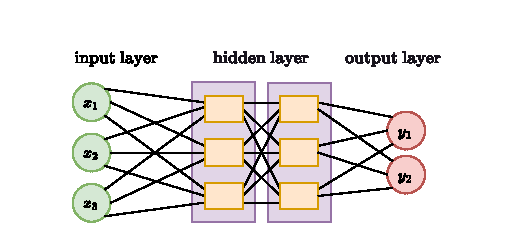
\includegraphics[width=0.7\linewidth]{Abschlussarbeit/Pictures/NN_mathematischausgerichtet.pdf}
    \caption{Illustration of a neural network. Adapted from \cite{zhou_machine_2021}.}
    \label{fig:IlNN}
\end{figure}

To understand the functional building blocks of neural networks, we now examine the internal structure of a single layer.
As illustrated in Figure~\ref{fig:layer}, a layer consists of multiple neurons that receive the same input vector \( x \in \mathbb{R}^{D^{(0)}} \), but apply different parameters.
If the layer comprises \( D^{(L)} \) neurons, that is, it produces an output vector of dimension \( D^{(L)} \), its parameters consist of a weight matrix \( W \in \mathbb{R}^{D^{(L)} \times D^{(0)}} \) and a bias vector \( b \in \mathbb{R}^{D^{(L)}} \).

The output of the layer is a vector \( y \in \mathbb{R}^{D^{(L)}} \), computed as
\[
z := Wx + b, \quad y := \sigma(z),
\]
where \( \sigma \) denotes the activation function, which is applied element-wise.

\begin{figure}[H]
    \centering
    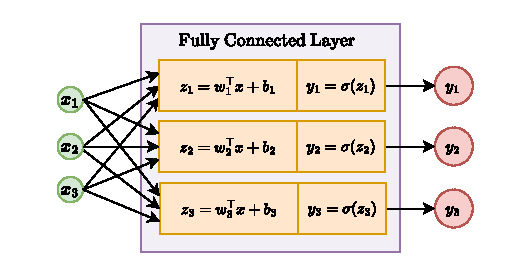
\includegraphics[width=0.7\linewidth]{Abschlussarbeit/Pictures/Layer_outp.pdf}
    \caption{Illustration of a neural networks layer}
    \label{fig:layer}
\end{figure}

At the core of each layer is the artificial neuron.
It performs a simple tow-step operation:
\begin{enumerate}
    \item Compute an affine transormation of the input,
    \item Apply a nonliear activation function.
\end{enumerate}

%Following Stevens et al.~\cite{antiga_deep_2020} notion, a single artificial neuron takes an input vector \( x = (x_1, x_2, \dots, x_n)^\top \in \mathbb{R}^n \), weights \( w = (w_1, w_2, \dots, w_n) \in \mathbb{R}^n \) and a bias term \( b \in \mathbb{R} \), and produces an output:
%\[
%y := \sigma(w^\top x + b).
%\]
%This defines a function \( f \colon \mathbb{R}^n \to \mathbb{R} \), where the codomain \( \operatorname{Im}(f) \) depends on the choice of \( \sigma \).  
%Typical activation functions and their properties are discussed in detail in Section~\ref{ActFunc}.  
%Figure~\ref{fig:artNeuron} shows an artificial neuron.





%\begin{figure}[h]
%    \centering
%    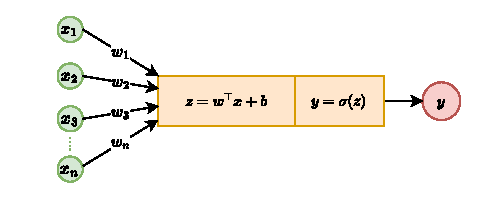
\includegraphics[width=0.7\linewidth]{Abschlussarbeit/Pictures/ArtificialNeuron_output.pdf}
%    \caption{Illustration of a neural networks artificial neuron}
%    \label{fig:artNeuron}
%\end{figure}



        \subsection{Activation Functions}\label{ActFunc}
        %In the previous section \ref{NN}, we have seen, that an artificial neuron maps input data to an output signal as $y=\sigma(W\cdot x+b)$.
%The simplest neural network would just be the linear operation $W\cdot x+b$.
%But if we use an activation function, we result on the one hand different slopes on the output functions. 
%On the other hand its function at the network's last layer is to focus the outputs of the previous linear operation inside a specified range.

%In the following we will discuss as Stevens et al. \cite{antiga_deep_2020} did, some different activation functions like the Heaviside's Threshold Function, \ac{RELU}, Sigmoid-Function or Tangens Hyperbolicus, which are visualized in figure \ref{fig:actFunc}.
%In the previous section (Section \ref{NN}), we saw that an artificial neuron maps an input vector $s\in \mathbb{R}^n$ to an output via the equation
%\[y = \sigma(w^\top x +b),\]
%where $w\in \mathbb{R}^n$ is a weight vector, $b\in \mathbb{R}$ is a bias term, and $\sigma$ is a non-linear activation function.

%Extending this to a fully layer with $m$ neurons, the model computes 
%\[y = \sigma(Wx+b),\]
%where $W\in \mathbb{R}^{m\times n}, b \in \mathbb{R}^m$ and $\sigma$ is applied element-wise.
In the previous section (Section \ref{NN}), we saw that a model  a fully connected layer computes outputs via the quation: \[y = \sigma(Wx+b),\] 
where $W\in \mathbb{R}^{m\times n}$ is the weight matrix, $b\in \mathbb{R}^m$ is a bias vector, and $\sigma$ is a non-linear activation function.



%If we don't consider the activation function, we only have an affine transformation  $Wx+b$, the model becomes purely linear.
%While such models are useful in simple settings (e.g. linear regression), they are limited in ther expressive power.
%A composition of linear functions is still linear, which means that even deep networks without non-linearities cannot represent complex patterns or decision boundaries. 

%The inclusion of non-linear activation functions is what gives neural networks the ability to approximate a wide class of functions, including any continuous function on a compact domain. %As shown in the Universal approximation theorem

If we don't consider the activation function, we only have an affine transformation  $Wx+b$, resulting in a purely linear model.While such models are useful in simple settings (e.g. linear regression), they are limited in ther expressive power.
A composition of linear functions is still linear, which means that even deep networks without non-linearities cannot represent complex patterns or decision boundaries. 

The inclusion of non-linear activation functions, particularly continuous sigmoidal functions endows neural networks with the expressive capacity to approximate a wide range of functions.
In fact, the Universal Approximation Theorem states that a feedforward neural network with a single hidden layer and a continuous sigmoidal activation function can uniformly approximate any continuous function defined on a compact domain, such as the unit hypercube $[0,1]^n$ \cite{cybenkot_approximation_nodate}.

Activation functions define the function space that a neural network can represent.
Their properties influence not only the expressive capacity of the network, but also its trainability, optimization dynamics, and numerical stability.

In the following, we discuss several commonly used activation functions as presented in Stevens et al. \cite{antiga_deep_2020}, including Heaviside's threshold function, the Rectified Linear Unit (ReLU), the sigmoid function, and the hyperbolic tangent. These functions are illustrated in Figure~ \ref{fig:actFunc}.

\begin{enumerate}
    \item[(a)] \textbf{Heaviside function}
    \begin{itemize}
        \item is a historically significant choice of activation function
        \item $\sigma(x) = H(x) :=
            \begin{cases} 
              0, & x < 0 \\
              1, & x \geq 0
            \end{cases}$
    \end{itemize}
    \item [(b)] \textbf{\ac{RELU}}
    \begin{itemize}
        \item one of the most used activation function in modern neural networks
        \item $\sigma(x)=\text{ReLU}(x):=\max\{0,x\}$
    \end{itemize}
    \item [(c)] \textbf{Sigmoid}
    \begin{itemize}
        \item commonly used activation function in early neural networks
        \item reason that activation functions are often labelled with $\sigma$
        \item $\sigma(x)=\text{Sigmoid}(x):=\frac{1}{1+e^{-x}}$
    \end{itemize}
    \item [(d)] \textbf{Hyperbolic tangent}
    \begin{itemize}
        \item similar to the sigmoid 
        \item $\sigma(x) = \tanh(x):=\frac{e^x-e^{-x}}{e^x+e^{-x}}$
    \end{itemize}
\end{enumerate}
\begin{figure}[h]
    \centering
    % Heaviside-Funktion
    \begin{subfigure}{0.24\textwidth}
        \centering
        \begin{tikzpicture}
            \begin{axis}[
                axis lines = middle,
                xlabel = $x$, ylabel = $H(x)$,
                width=4cm, height=4.5cm
            ]
            \addplot[black, thick, domain=-6:6, samples=200] {x >= 0 ? 1 : 0};
            \end{axis}
        \end{tikzpicture}
        \caption{Heaviside}
    \end{subfigure}
    \hfill
    % ReLU-Funktion
    \begin{subfigure}{0.24\textwidth}
        \centering
        \begin{tikzpicture}
            \begin{axis}[
                axis lines = middle,
                xlabel = $x$, ylabel = $f(x)$,
                width=4cm, height=4.5cm
            ]
            \addplot[red, thick, domain=-6:6, samples=200] {max(0, x)};
            \end{axis}
        \end{tikzpicture}
        \caption{ReLU}
    \end{subfigure}
    \hfill
    % Sigmoid-Funktion
    \begin{subfigure}{0.24\textwidth}
        \centering
        \begin{tikzpicture}
            \begin{axis}[
                axis lines = middle,
                xlabel = $x$, ylabel = $\quad \sigma(x)$,
                width=4cm, height=4.5cm
            ]
            \addplot[blue, thick, domain=-6:6, samples=200] {1 / (1 + exp(-x))};
            \end{axis}
        \end{tikzpicture}
        \caption{Sigmoid}
    \end{subfigure}
    \hfill
    % Tanh-Funktion
    \begin{subfigure}{0.24\textwidth}
        \centering
        \begin{tikzpicture}
            \begin{axis}[
                axis lines = middle,
                xlabel = $x$, ylabel = $\quad\tanh(x)$,
                width=4cm, height=4.5cm
            ]
            \addplot[green, thick, domain=-6:6, samples=200] {tanh(x)};
            \end{axis}
        \end{tikzpicture}
        \caption{Tanh}
    \end{subfigure}
    \caption{Activation functions}
    \label{fig:actFunc}
\end{figure}

\newpage

There exists some common multivariate functions as Softmax and Maxpool, too.
His multivariate functions operate on vectors and tensor and are commonly used to transform a vector of real-values scores into a probability distribution over classes. 
\begin{enumerate}
    \item[(a)] \textbf{Softmax}
    \begin{itemize}
        \item For \( \lambda > 0 \), the scaled softmax is defined as
        \[
            \operatorname{softmax}_\lambda: \mathbb{R}^n \to [0,1]^n,\quad 
            \operatorname{softmax}_\lambda(x)_i = \frac{e^{\lambda x_i}}{\sum\limits_{j=1}^{n} e^{\lambda x_j}},\quad \forall i \in \{1, \dots, n\}.
        \]
    \end{itemize}
	\item[(b)] \textbf{Maxpool operation}
	\begin{itemize}
		\item The maxpool function is defined as
		\[
		\operatorname{maxpool}: \mathbb{R}^n \to \mathbb{R}^m, \qquad 
		\operatorname{maxpool}(x)_i = \max_{j \in I_i} x_j 
		\quad \text{for all } i \in \{1, \dots, m\},
		\]
		where \( I_i \subset \{1, \dots, n\} \) defines the pooling region.
	\end{itemize}
\end{enumerate}


\subsection{Training Process}
After introducing layers and non-linear activation functions, we now have all required components for a neural network to approximate complex functions.
However, in order to fit an actually given task such as mapping inputs to outputs, we shall need to determine appropriate values for the networks weights and biases.
This is where we use the trainings process. 
The goal of training process is to adjust the parameters of a neural network that explains the best relationship between the given inputs and outputs.
This is achieved by computing the error between the networks output and the target values using a loss function $\mathcal{L}$ and then propagating this error backwards through the network to update the parameters, this process is known as backpropagation. 
During backpropagation, the network applies the chain rule to pass the error from the output layer back to the earlier layers, adjusting weights and biases along the way in order to minimize the loss.



A loss function \(\mathcal{L}\) measures the discrepancy between the network's predicted output and the true target value.  
Its purpose is to guide the training process by quantifying how wrong the network's predictions are.

It measures the  loss of the model and will be minimized during the training process.
Common choices of loss functions, as presented in \cite{zhou_machine_2021}, include:
%Therefore, the model adjusts the weights using different approaches, like squared error loss or cross entropy, as presented in \cite{zhou_machine_2021}.

\begin{enumerate}
    \item[(a)] \textbf{Squared Error Loss}
    \begin{itemize}
        \item Measures the squared difference between predicted and target values.
        \item Often used in regression settings, but can also be applied to compare continuous representations in higher-dimensional spaces.
        \item Defined as
        \[
        \mathcal{L}_{\operatorname{SquareErr}}(y, \hat{y}) = \sum_{i = 1}^{n} \| y_i - \hat{y}_i \|^2.
        \]
    \end{itemize}
    
    \item[(b)] \textbf{Cross Entropy Loss}
    \begin{itemize}
        \item Used for classification tasks involving discrete probability distributions.
        \item Let $p = (p_1, \dots, p_k)$ and $q = (q_1, \dots, q_k)$ be discrete probability distributions over $k$ classes.
        \item Defined as
        \[
        \mathcal{L}_{\operatorname{CrossEnt}}(p, q) = -\sum_{i=1}^{k} p_i \ln q_i.
        \]
    \end{itemize}
    
    \item[(c)] \textbf{Huber Loss}
    \begin{itemize}
        \item Combines properties of squared error loss and absolute error loss..
        \item Less sensitive to outliers than squared error loss.
        \item Introduced by Peter J. Huber in his foundational work on robust statistics \cite{gokcesu2021generalizedhuberlossrobust}
        \item Defined for a threshold $\delta > 0$ as
        \[
        \mathcal{L}_{\operatorname{Huber}}(y, \hat{y}) =
        \sum_{i=1}^{n}
        \begin{cases}
            \frac{1}{2} (y_i - \hat{y}_i)^2 & \text{if } |y_i - \hat{y}_i| \leq \delta, \\
            \delta \left( |y_i - \hat{y}_i| - \frac{1}{2} \delta \right) & \text{otherwise}.
        \end{cases}
        \]
    \end{itemize}
\end{enumerate}


We now formalize the training task. 
Let $\mathcal{D} := \{(x_i, y_i)\}_{i=1}^n$ be a dataset of input-output pairs, where $x_i$ are the inputs and $y_i$ the corresponding labels.  
Let $f(x, \theta)$ be a neural network parameterized by $\theta$ that maps inputs to outputs.  
We define the set of all trainable parameters, i.e., the weight matrices and bias vectors of each layer $l = 1,\dots,L$, as
\[
\theta := \{(W^{(l)}, b^{(l)}) \mid W^{(l)} \in \mathbb{R}^{m_l \times n_l},\ b^{(l)} \in \mathbb{R}^{m_l} \}.
\]

Following Smets~\cite{smets2024mathematicsneuralnetworkslecture}, we define the sample-wise loss as
\[
\tilde{f}_i(\theta) := \mathcal{L}(y_i, f(x_i, \theta)) \quad \text{for } i = 1, \dots, n,
\]
and define the overall training objective as minimizing the average loss across the dataset:
\[
\min_{\theta} \frac{1}{n} \sum_{i=1}^{n} \tilde{f}_i(\theta).
\]

To solve this optimization problem, gradient-based methods such as \emph{stochastic gradient descent} (SGD) are commonly used.  
These methods update the model parameters iteratively in the direction that reduces the loss.

Concretely, the parameters \(\theta\) are updated via the rule
\[
\theta \leftarrow \theta - \eta \cdot \nabla_\theta \left( \frac{1}{n} \sum_{i=1}^{n} \tilde{f}_i(\theta) \right),
\]
where \(\eta > 0\) is the learning rate that controls the step size.  
The required gradients \(\nabla_\theta \mathcal{L}(y_i, f(x_i, \theta))\) are efficiently computed using \emph{backpropagation}, which applies the chain rule to propagate derivatives through the network layers.
In classical \emph{gradient descent}, the full gradient over the entire dataset is used in each step. 
This becomes computationally expensive for large datasets.
In contrast, \emph{stochastic gradient descent (SGD)} approximates this full gradient by computing it on small random subsets of the data, called mini-batches.
This introduces some noise into the updates but allows for faster and more scalable training.

One widely used variant of SGD is the \emph{Adam optimizer} \cite{kingma2017adammethodstochasticoptimization}, which adaptively adjusts the learning rate for each parameter based on estimates of the first and second moments of the gradients.
Adam combines the benefits of two earlier methods, and often leads to faster convergence and more stable training, especially in deep networks.



The following code snippet~\ref{lst:train-func} shows the training routine of a neural network used to learn a nonlinear transformation for intrinsic homotopy, which will be discussed in detail in Chapter~\ref{ISA}.
\lstinputlisting[
  caption={Code snippet showing how to train a neural network},
  label={lst:train-func},
   basicstyle=\small\ttfamily,
  firstline=1,
  lastline=55
]{Abschlussarbeit/Text/NeuralNetwork/train_NN_.py}



		\newpage
        \section{Types of Neural Networks}\label{ToNN}
        In the previous sections, we discussed artificial neural networks in general.  
There exist various types of neural networks, distinguished by their architecture and typical use cases.  
The following list gives a brief overview of some common types, as presented by Goyal et al.~\cite{goyal_deep_2018}:

\begin{enumerate}
    \item[(a)] \textbf{Feedforward Neural Networks (FNNs)} are the simplest type of neural network.  
    Data flows in one direction—from the input layer, through one or more hidden layers, to the output layer—without cycles or loops.

    \item[(b)] \textbf{Convolutional Neural Networks (CNNs)} are commonly used for image and handwriting recognition.  
    They apply convolutional filters to local regions of the input to extract features, which are then used to build hierarchical representations.

    \item[(c)] \textbf{Recurrent Neural Networks (RNNs)} are designed to process sequential data.  
    Each time step receives an input and the output of the previous step, allowing the network to retain a form of memory.  
    This makes RNNs particularly suitable for time series, language, and other temporally dependent data.

    \item[(d)] \textbf{Transformers} \cite{vaswani_attention_2023} are modern neural network architectures that rely entirely on attention mechanisms rather than recurrence or convolution.  
    They allow parallel processing of sequences and have achieved state-of-the-art performance in natural language processing tasks such as translation, summarization, and question answering.
\end{enumerate}


        
        \chapter{Natural Language Processing}\label{NLP}
        In this thesis, we focus on the similarity analysis of language encoders, which are central components of modern \ac{NLP} systems. 
Language encoders transform raw text into structured vector representations that can be processed by machine learning models. 
Since our approach is based on comparing and transforming these encoders, they form a foundational element of this work.

\acf{NLP} enables machines to interpret, process, and generate human language. 
Unlike structured data, natural languages present a wide variety of problems that vary from language to language. 
Structuring or extracting meaningful information from free text represents a great solution, if it is done in the right manner.
Historically, \ac{NLP} relied on rule-based systems that analyzed grammatical structure using syntactic parsers and manually designed algorithms. 
These approaches were often limited in scalability and adaptability across different languages and contexts.
Previously, computer scientists broke a language into its grammatical forms, such as parts of speech, phrases, etc., using complex algorithms. 
With the rise of deep learning, data-driven methods have largely replaced rule-based systems.
Modern \ac{NLP} models can learn complex patterns directly from text corpora and perform tasks such as machine translation, text summarization, question answering, and speech recognition with remarkable accuracy~\cite{goyal_deep_2018}.
This chapter provides a technical introduction to the foundations of \ac{NLP}. Section~\ref{LangMod} introduces the concept of language encoders, which transform text into structured vector representations. 
Section~\ref{TM} then presents transformer-based models, the current state-of-the-art architecture in \ac{NLP}.
%In the end, in section \ref{TMaiA} we present real-word models that are build on the transformer and are used withing this thesis. 

        \section{Language Modeling}\label{LangMod}
        %\section{Formalizing Language Encoder}        
        In this section, we introduce the mathematical building blocks of modern language models. 
Intuitively, a \emph{language encoder} is a function that transforms text into numbers. 
This is necessary because computers cannot directly work with text, they need numerical representations.

To do so, we use Cotterells et al. publication \cite{cotterell_formal_2024} as baseline and define the important tools in language modelling if not referenced differently as they did.

\begin{definition}[Language Encoder]
A \textbf{language encoder} is a function
\[
h:\Sigma^* \rightarrow V
\]
that maps text strings to vectors of real value. 
Here, $\Sigma^*$ denotes the set of all possible sequences of characters from a finite alphabet $\Sigma$, and $V = \mathbb{R}^D$ is a $D$-dimensional real vector space.
\end{definition}

For example, the sentence “language is powerful” might be mapped to a 768-dimen\-sional vector such as $(0.1, -0.3, \dots, 0.2)$.


We define:

\begin{itemize}
    \item $\mathcal{E}_V := V^{\Sigma^*}$: the set of all such encoders.
    \item $\mathcal{E}_b := \{ h \in \mathcal{E}_V \mid h(\Sigma^*) \text{ is bounded} \}$: the subset of encoders that do not produce arbitrarily large vectors.
\end{itemize}

A \textbf{language model} is a probability distribution over all possible texts. 
It allows us to answer questions like: “How likely is this sentence?” or “What word should come next?”

\begin{definition}[Language Model]
A \textbf{language model} is a probability distribution
\[
p_{\mathrm{LM}}: \Sigma^* \rightarrow [0,1]
\]
that assigns probabilities to strings over the alphabet $\Sigma$.
\end{definition}

A common type of language model is the \emph{autoregressive model}, which predicts the next word in a sentence one step at a time. 
This process stops when a special end-of-sequence symbol (\texttt{EOS}) is generated.


\begin{definition}[Autoregressive Language Model]
Given a sequence $y = (y_1, \dots, y_T)$, an autoregressive model defines:
\[
p_h^{\mathrm{LM}}(y) = p_h(\texttt{EOS} \mid y) \cdot \prod_{t=1}^T p_h(y_t \mid y_{<t})
\]
The conditional probabilities are parametrized using a language encoder $h$ as:
\[
p_h(y_t \mid y_{<t}) = \operatorname{softmax}(E h(y_{<t}))_{y_t}
\]
where $E \in \mathbb{R}^{(|\Sigma|+1) \times D}$ is a learned embedding matrix.
\end{definition}

This formulation is used in models like GPT.


An alternative training strategy is \emph{masked language modeling}, where some words in a sentence are replaced with a special token like \texttt{[MASK]} and the model must guess them.



%\begin{definition}[Masked Language Model]
%A \textbf{masked language model} estimates:
%\[
%p_h(y_t \mid y_{<t}, y_{>t}) = \operatorname{softmax}(E h(y_{<t} \circ [\texttt{MASK}] \circ y_{>t}))_{y_t}
%\]
\begin{definition}[Masked Language Model]
Let \( y = (y_1, \dots, y_T) \) be a sequence of tokens from a vocabulary \( \mathcal{V} \), and let \( t \in \{1, \dots, T\} \) be a randomly selected position to mask.
Let \( y_{\setminus t} := (y_1, \dots, y_{t-1}, \texttt{[MASK]}, y_{t+1}, \dots, y_T) \) denote the input sequence with the \( t \)-th token replaced by a special \texttt{[MASK]} token.
A \textbf{masked language model (MLM)} estimates the conditional probability
\[
p_h(y_t \mid y_{\setminus t}) = \operatorname{softmax}(E\, h(y_{\setminus t}))_{y_t},
\]
where:
\begin{itemize}
    \item \( h \colon \mathcal{V}^T \to \mathbb{R}^D \) is a language encoder that maps the masked sequence \( y_{\setminus t} \) to a hidden representation;
    \item \( E \in \mathbb{R}^{|\mathcal{V}| \times D} \) is a learned projection from the hidden space to vocabulary logits;
    \item The softmax is applied on the vector \( z := E\, h(y_{\setminus t}) \in \mathbb{R}^{|\mathcal{V}|} \): \[ \operatorname{softmax}(z)_v:= \frac{\exp(z_v)}{\sum\limits_{v' \in \mathcal{V}} \exp(z_{v'})} \quad \text{for } v \in \mathcal{V}.
    \]\end{itemize}
\end{definition}


\textbf{Example:}

\texttt{The students [MASK] to learn about language models.}

The model should assign high probabilities to words like \textit{want} or \textit{like}. This task encourages the model to understand both the left and right context of a word.
        %\section{Recurrent Neural Networks}\label{RnnLstm}
If we feed a network with a string, it produces a binary vector as an output.
Consequently, the order of the words are lost.
Recurrent Neural networks are kind of language encoder, that can process the sequence of data.
The recurrent layer of an \ac{RNN} re-introduces the words order into the networks internal.
Furthermore, the inputs are distinguished chronologically by an index $t: x_{t-1},x_t, x_{t+1}$.
And a second matrix $U$, such that values can be sent to the next layer is used \cite{haralambous_course_2024}:
\begin{equation}
    \sigma(Ax_t+Ux_{t-1}+b)
\end{equation}

The architecture of \ac{RNN}, is illustrated in Figure \ref{fig:RNN}.
It implies that the temporal sequence of the input data has an influence on the result.
For this purpose, information from one processing step is transferred with a time delay to the processing of the next one using the following pattern.

\begin{figure}[h]
   \centering
   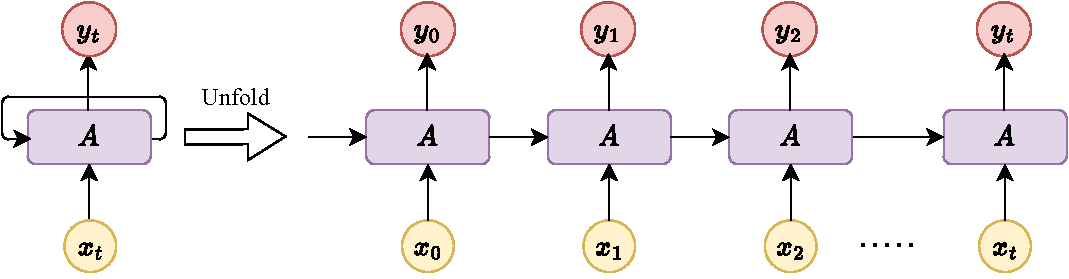
\includegraphics[width=0.8\linewidth]{Abschlussarbeit/Pictures/RNN.drawio.pdf}
   \caption{\ac{RNN}, output of first influences the second \cite{BiLSTM}}
   \label{fig:RNN}
\end{figure}

Especially with backprobagation, \ac{RNN}s have the disadvantage that the gradients either vanishes or explode if the length of the sequence is long enough.
This leads to a very slow manner of the models training.
When this occurs, \ac{LSTM} networks can help. 
They are a type of \ac{RNN} architecture that uses an internal memory that stores the inputs that were fed to the model at previous time steps.

Ideally, this will solve the problem of the disappearing or exploding gradient.

\ac{RNN} can only process word by word and this is why they are operating very slow, compared to transformer, that are able to process a complete sentence 
\ac{LSTM} \cite{originalLSTM_book} are special \ac{RNN} cells, that uses an internal memory and multiplicative gates.
As Smagulova and James \cite{LSTM}, we explain \ac{LSTM} by the use of figure \ref{fig:LSTM}, that illustrates the unit architecture of an original \ac{LSTM} with memory cell and two gates. 

\begin{figure}[htb]
\begin{minipage}{7.5cm}
 \centering
   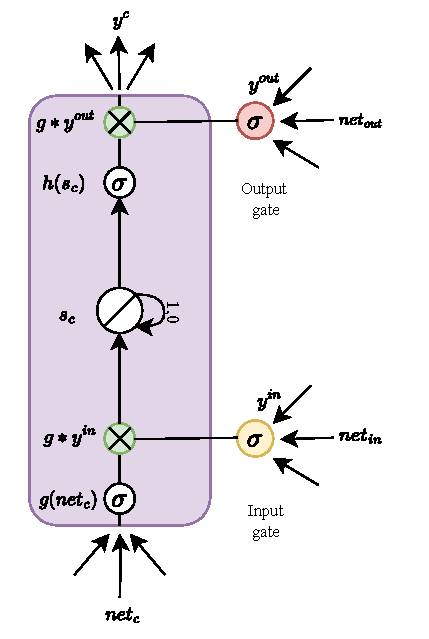
\includegraphics[width=\linewidth]{Abschlussarbeit/Pictures/LSTMoriginal.pdf}
   \caption{Original \ac{LSTM} \cite{LSTM}}
   \label{fig:LSTM}
\end{minipage}
\hfill
\begin{minipage}{6.5cm}

The self-connected linear unit, denoted by $s_c$, which is also called constant error carousel, the hear of a memory block.
The input gate, with weighted inputs, is denoted as $net_{in}$ and the output as $y^{in}$
The output gate with weighted input is denoted as $net_{out}$ and $y^{out}$ shapes the output of the cell $y^c$.
$h$ is a differentiable function, that scales $x_c$.
$g$ is a function, that squashes the weighted input of the cell $net_{c}(t)$.
\end{minipage}
\end{figure}


Originally, \ac{LSTM} is subjected to some limitations due to the linear nature of $s_c$.
Consequently, a forget gate layer was included to delete and forget unneeded information. 
There is a similarity between the behaviour of \ac{LSTM} cell with forget gate and the standard \ac{LSTM} with exception of cell state/ internal memory $s_c(t)$/ $c_t$, which includes an impact of an output of the forget gate $y^\varphi/f_t$.
We can define the two parameters as follows:

\begin{equation}
    \begin{split}
            & s_{c_j}(t) = y^{\varphi_j} (t) s_{c_j(t-1)}+y^{in_j}(t)g(net_{c_j}(t))\\
            \\
            & y^{\varphi_j}(t)=f_{\varphi_j}(net_{\varphi_j}) 
    \end{split}
\end{equation}


The forget gate's behaviour is similar to standard \ac{LSTM}.
In this process, the cell input $x_t$ at time $t$ concatenates with output $h_{t-1}$ of the previous cell at previous time step $t-1$.
$h_{t-1}$ is denoted by hidden state. 
The resulting vector traverses input nodes $g_t$, forget gate $f_t$, input gate $i_t$ and output gates $o_t$.
Afterwards, the forget gate decides whether the cell data $c_{t-1}$ from a previous time step will be kept or blocked.
        \begingroup
\frametitle{Wie funktionieren neuronale Netze in der Praxis?}
\begin{frame}[plain]
	\vfill
	\begin{minipage}[c]{0.53\linewidth}
		\begin{itemize}
			\item Datengesteuerte, nichtlineare Funktionsapproximation
			\item Aufbau aus Layern \( f_1, f_2, \dots, f_L \)
			\item Architektur als Komposition:
			\[
			g(x) = f_L \circ f_{L-1} \circ \dots \circ f_1(x)
			\]
		\end{itemize}
	\end{minipage}
	\hfill
	\begin{minipage}[c]{0.44\linewidth}
		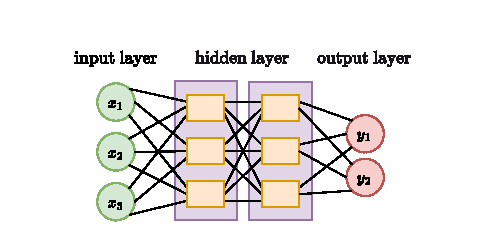
\includegraphics[width=0.95\linewidth]{BilderPräsentation/NN_ausgerichtet.drawio.pdf}
		\begin{itemize}\item []	{\scriptsize Schematische Darstellung eines neuronalen Netzwerks: Eingabe \(x_1, x_2, x_3\) wird durch eine Sequenz nichtlinearer Layer in Ausgaben \(y_1, y_2\) transformiert.} \end{itemize}
		
	\end{minipage}
	\vfill
\end{frame}
\endgroup


\begingroup
\frametitle{ Neuronale Netze: Black Box?}
\begin{frame}[plain]
	\centering
	
	\uncover<1->{	\begin{tikzpicture}[scale=1, every node/.style={font=\small}]
			% Input Text
			\node at (-5.5, 2) {Input $x \in \mathbb{R}^n$};
			
			% Pfeil von Input zum Hut
			\draw[very thick, ->] (-3,2) -- (-1.8,2);
			
			% Magic Hat Image
			\node at (0, 2.6) {
\includegraphics[width=2.2cm]{BilderPräsentation/magic_hat.png}};
			\node at (0, 1.3) {\footnotesize Neural Network};
			
			% Pfeil von Hut zu Output
			\draw[very thick, ->] (1.4,2) -- (2.8,2);
			
			% Output Text
			\node at (5.2, 2) {Output $g(x)$};
	\end{tikzpicture}}
	
	\vspace{1.5em}
	\uncover<1->{	\textbf{Frage:} Können neuronale Netze wirklich jede Funktion lernen?}
	
\end{frame}
\endgroup

\begingroup
\frametitle{Universal Approximation Theorem}
\begin{frame}
	\vspace{-1.3em}
	\begin{minipage}[t]{0.3\linewidth}
		\centering
		\vspace{0.5em}
		
\includegraphics[width=2.3cm]{BilderPräsentation/magic_hat.png}\\[0.5em]
	\end{minipage}%
	\hfill
	\begin{minipage}[t]{0.7\linewidth}
		\begin{block}{Universal Approximation Theorem~\cite{cybenko:hal-03753170}}
			\small
			Für jede stetige Funktion \( g \in C([0,1]^n) \) und jedes \( \varepsilon > 0 \)
			existiert ein neuronales Netz \( f \) der Form
			\[
			f(x) = \sum_{j=1}^{m} w^{(2)}_j\, \sigma\big( x^\top w^{(1)}_j - b_j \big),
			\]
			sodass \( \|g - f\|_\infty < \varepsilon \).
		\end{block}
	\end{minipage}
	

	{\tiny Quelle: Cybenko, “Approximation by superpositions of a sigmoidal function”, \textit{Mathematics of Control, Signals and Systems}, 1989~\cite{cybenko:hal-03753170}}
	
\end{frame}
\endgroup




\section{Natural Language Processing}
\frame{\tableofcontents[currentsection]}
\begingroup
\frametitle{Definition: Language Encoder}

\begin{frame}
	\begin{block}{Language Encoder}
		\small
		Ein \textbf{Language Encoder} ist eine Abbildung
		\[
		h : \Sigma^* \rightarrow \mathbb{R}^D,
		\]
		die Texte \(x \in \Sigma^*\) aus einem Alphabet \(\Sigma\) auf Vektoren \(h(x)\) im Repräsentationsraum \(\mathbb{R}^D\) abbildet.
		
		\vspace{0.3em}
		Die Menge aller solcher Encoder ist \(\mathcal{E}_V := V^{\Sigma^*}\).
		
	\end{block}
\end{frame}

\endgroup


\begingroup
\frametitle{Sprachverarbeitung mit Encoder-Decoder-Modellen}
\begin{frame}
	\centering
	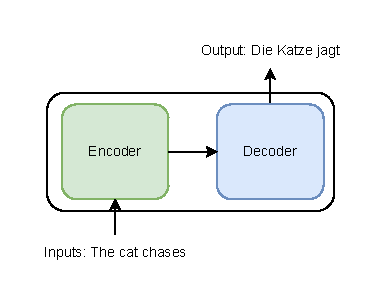
\includegraphics[width=0.4\linewidth]{BilderPräsentation/encoder_decoder.pdf}
	
	\begin{itemize}
		\item Encoder erzeugt eine Vektorrepräsentation aus dem Input-Text
		\item Decoder generiert daraus eine Zielsprache (z.\,B.\ Übersetzung)
		\item Modell lernt die Repräsentation durch Training auf großen Textdaten
	\end{itemize}
\end{frame}


\endgroup

        \chapter{Preliminaries}\label{Preliminaries}
        In order to formally develop the concepts of intrinsic and extrinsic homotopy for language encoders, we first need some basic mathematical notions.
The aim of this chapter is to provide a theoretical framework in which encoders can be compared with respect to their similarity using transformations. 
To this end, we first introduce \emph{hemi-metric spaces} in Section ~\ref{HMS} , which enable an asymmetric distance function between language encoders.
This structure allows us to measure similarities without necessarily requiring symmetry or the triangle inequality, properties that are often not given in practical comparison scenarios.
Based on this, we define the norms and distances in Section ~\ref{ND} in the space of language encoders.
These measures are crucial for mathematically quantifying differences between encoders and analyzing transformations. %Der Copilot schlägt hier immer analyzing vor und die Rechtschreibprüfung sagt immer analysing
A central concept, the so-called \emph{Specialisation Quasi-Ordering}, which is a special form of preordering derived from the hemi-metric structure, is presented in Section ~\ref{sec:sqp}.
It describes whether one encoder can be completely transformed into another one.
Finally, we motivate \emph{homotopy} in Section ~\ref{UHtMS} to measure similarity.


\section{Hemi-Metric Spaces}\label{HMS}
In the following, we will use the definition of metrices and a hemi-metric as tom Dieck \cite{dieck_mengentheoretische_top} defined.
Further, we consider Metric Spaces $(X,d)$, that is, a set $X$ and a metric $d$ operation on $X$.
A metric on a set $X$ is a mapping $d:X\times X \rightarrow [0,\infty[$ that satisfies the known axioms:
\begin{itemize}
    \item [M1] $d(x,y) > 0$ and $d(x,y) = 0 \Leftrightarrow x=y$
    \item [M2] $d(x,y)=d(y,x) \quad \forall x,y\in X$
    \item [M3] $d(x,z) \leq d(x,y) + d(y,z) \quad \forall x,y,z \in X$
\end{itemize}

If there is a map $d:X\rightarrow \overline{\mathbb{R}}_+$, that means that the metric can be equal to $\infty$ and we denote it as an \textbf{extended metric}.
A \emph{hemi-metric} or \emph{Lawvere metric}~\cite{lawvere_metric_1973} is a generalized distance function that relaxes the symmetry requirement of a metric.

\begin{definition}[Hemi-metric / Lawvere metric]\label{def:hemi_metric}
Let \( X \) be a set.  
A function \( d \colon X \times X \to \overline{\mathbb{R}}_+ \) is called a \emph{hemi-metric} (or \emph{Lawvere metric}~\cite{lawvere_metric_1973}) if it satisfies the following two axioms:
\begin{itemize}
    \item [H1] \( d(x, x) = 0 \) for all \( x \in X \),
    \item [H2] \( d(x, z) \le d(x, y) + d(y, z) \) for all \( x, y, z \in X \).
\end{itemize}
Note that symmetry is not required, i.e., it may hold that \( d(x, y) \ne d(y, x) \).  
If the codomain includes \( \infty \), we call \( d \) an \emph{extended hemi-metric}.
\end{definition}



This relaxation allows us to define an asymmetric notion of distance between representations.
In particular, we can formalize how far a language encoder \( h \) is from the set of all possible transformations of another encoder \( g \).
To this end, the hemi-metric is lifted from individual elements \( x \in X \) to subsets of \( X \).
\begin{definition}[Hausdorff-Hoare map]\label{def:hausdorffHoareMap}
Let $(X,d)$ be a hemi-metric space, and let $E, E' \subset X$ be non-empty subsets.  
The \emph{Hausdorff-Hoare map} is the function
\[
d^{\mathcal{H}}(E, E') := \sup_{x \in E} \inf_{y \in E'} d(x, y),
\]
that defines a hemi-metric on $\mathcal{P}(X) \setminus \{\emptyset\}$.
\end{definition}

If $E$ is considered as a singleton set $\{x\}$, we will write $d^\mathcal{H}(x,E')$ instead of $d^\mathcal{H}(\{x\},E'):=\inf\limits_{g\in E'}d(x,y)$

%Further, if we want to define a hemi-metric on a set $X$ by embedding $X$ into the power set of a second space $Y$ where a hemi-metric exists.
%The Hausdorff-Hoare map based on the hemi-metric of $Y$ can be used after $X$ is embedded to define a hemi-metric in $X$ through the images of $x \in X$.
If a set \( X \) does not itself carry a hemi-metric, but can be embedded into the power set of a second space \( Y \) that does, we can induce a hemi-metric on \( X \) via this embedding.  
Specifically, let \( \varphi: X \to \mathcal{P}(Y) \setminus \{\emptyset\} \) be an embedding of \( X \) into non-empty subsets of \( Y \).  
Then a hemi-metric on \( X \) can be defined by
\[
d_X(x, x') := d^\mathcal{H}(\varphi(x), \varphi(x')),
\]
where \( d^\mathcal{H} \) is the Hausdorff–Hoare map induced by the hemi-metric on \( Y \).


\section{Norm and Distances}
\label{ND}
%To follow the hemi-metric recipe, it is required, to define a hemi-metric on the individual elements.
%Let \( V \) be a finite-dimensional \( \mathbb{R} \)-vector space, equipped with a norm \( |\cdot|_V \). Since all norms on finite-dimensional spaces are equivalent, we fix one such norm for the remainder. 

%We consider the space of encoder functions \( \mathcal{E}_V \subset \{ h : \Sigma^* \to V \} \), equipped with the norm:
%\[
%\|h\|_\infty := \sup_{y \in \Sigma^*} |h(y)|_V,
%\quad \text{and corresponding metric} \quad
%d_\infty(h, g) := \|h - g\|_\infty.
%\]
%Assuming that \( \mathcal{E}_V \) is closed under this norm, the space \( (\mathcal{E}_V, d_\infty) \) is a complete metric space. This follows from the completeness of \( V \) and the definition of the supremum norm on function spaces.


As is well known, every norm on a real vector space induces a metric via \( d(x, y) := \|x - y\| \).  
Since all norms on a finite-dimensional \(\mathbb{R}\)-vector space \(V\) are equivalent \cite{lang_algebra_2002}, we will work with a fixed norm \(|\cdot|_V\) on \(V\) in the following.


%As all norms in the $\mathbb{R}$-vector space $V$ are equivalent, the norm $|\cdot|_V$ on $V$ will be considered in the following.

We further define the extended norm
\[
\|h\|_\infty := \sup_{y \in \Sigma^*} |h(y)|_V,
\]
and the induced metric
\[
d_\infty(h, g) := \|h - g\|_\infty
\]

on the space \(\mathcal{E}_V\), which consists of all functions \(h : \Sigma^* \to V\) with finite \(\|\cdot\|_\infty\)-norm.
%A metric space where every Cauchy sequence converges to a point within the space. 
%That is given by the fact that $|\cdot|_V$ is a norm and the completeness of $V$.

Equipped with this metric, \((\mathcal{E}_V, d_\infty)\) forms a complete metric space, meaning that every Cauchy sequence in \(\mathcal{E}_V\) converges to a limit within the space.  
This follows from the fact that \(V\) is a finite-dimensional normed space and hence complete.
This property will later be used to argue the existence of certain infima in \(\mathcal{E}_V\).



For the subordinate matrix norm we write $\|\cdot\|_V: GL(V) \rightarrow \mathbb{R}_+$, where $GL(V)$ denotes the set of invertible $D\times D $ matrices.
It is defined as \[\|W\|_V=\sup_{v\in V\setminus \{0\}}\frac{|W v|_V}{|v|_V}.\]
We consider $V$ as an affine space and set $\text{Aff}(V)$ for the group of affine transformations of $V$, by abuse of language, if we forget about the special role that the zero vector has.

A map $v\mapsto Wv +b$ is called an affine transformation $\psi$ on $V$ for $W\in GL(V)$ invertible and $b \in V$.
The transformation consists of a linear part $\psi_{lin}:=W$ and a translation part $\psi_t:v\mapsto v+b$.
Further, $\mathcal{T}\subset \text{Aff}(V)$ denotes the subgroup of translation.
There is also a natural left action on $\text{Aff}(V)$ on $\mathcal{E}_V$.
I.e. $\text{Aff}(V)\times \mathcal{E}_V\rightarrow \mathcal{E}_V, h \mapsto \psi\circ h$, such that there exists an identity element $e$ on $\text{Aff}(V)$, where $e\cdot h = h \quad \forall h\in \mathcal{E}_V$ and $\psi_1\cdot(\psi_2\cdot h)=(\psi_1\psi_2)\cdot h \quad \forall \psi_1,\psi_2 \in \text{Aff}(V)\ \text{ and } h \in \mathcal{E}_V$.

\section{Specialization Quasi-ordering and Pre-ordering}\label{sec:sqp}
In this section, we formalize the notion of specialization quasi-ordering and show that it induces a preorder.
This structure will be used to define various homotopies on language encoders in later sections.
We follow the exposition of Goubault-Larrecq in \cite{goubault-larrecq_non-hausdorff_nodate}.

We begin with a brief reminder of the concept of a topological space.
A \emph{topological space} is a set $X$ equipped with a collection of subsets, called \emph{open sets}, that satisfies the following properties:
\begin{itemize}
\item The empty set $\emptyset$ and the full set $X$ are open.
\item Arbitrary unions of open sets are open.
\item Finite intersections of open sets are open.
\end{itemize}
This collection of open sets defines the topology on $X$.

\begin{definition}[Base]
        Let $X$ be a topological space, and $\mathcal{B}$ be a family of open subsets of $X$.
        If every open set is a union of elements of $\mathcal{B}$, $\mathcal{B}$ is a \emph{base} of the topology. 
\end{definition}

\begin{lemma}[Characterization of a Basis]\label{lem:basis_characterization}
A family \(\mathcal{B}\) of subsets of a topological space \(X\) is a basis of the topology if and only if for every open set \(U \subseteq X\) and every point \(x \in U\), there exists an element \(V \in \mathcal{B}\) such that \(x \in V \subseteq U\).
\end{lemma}

\begin{proof}
Let \(U\) be open and \(x \in U\). 
By assumption, there exists \(V_x \in \mathcal{B}\) with \(x \in V_x \subseteq U\).  
Using the Axiom of Choice, pick such a \(V_x\) for each \(x \in U\), and write \(U = \bigcup\limits_{x \in U} V_x\).

Suppose \(\mathcal{B}\) is a basis, and let \(U = \bigcup\limits_{i \in I} V_i\) with \(V_i \in \mathcal{B}\). 
For any \(x \in U\), there exists some \(i \in I\) such that \(x \in V_i\). Let \(V := V_i\), then \(x \in V \subseteq U\).
\end{proof}


\begin{definition}[Specialization Quasi-ordering]\label{def:quasi-ordering}
Let $X$ be a topological space. 
The specialization quasi-ordering on $X$ is defined by:
\[
x \gtrsim y \quad \text{if and only if} \quad \text{every open set containing } x \text{ also contains } y.
\]
\end{definition}

This quasi-ordering induces a preorder on $X$, as stated in the following lemma.


\begin{lemma}[Preorder]\label{lemma:preorder}
The specialization quasi-ordering is a preorder; that is, it is reflexive and transitive.
\end{lemma}


\begin{proof}
Let $\gtrsim$ denote the specialization quasi-ordering.

\textbf{Reflexivity:} For any $x \in X$, every open set containing $x$ trivially contains $x$ itself, so $x \gtrsim x$.

\textbf{Transitivity:} Suppose $x \gtrsim y$ and $y \gtrsim z$. Let $U$ be an open set containing $x$. Then, by definition of $\gtrsim$, $y \in U$, and hence $z \in U$. Therefore, $x \gtrsim z$.
\end{proof}


Now consider a hemi-metric $d$ on a set $X$. We define open balls by
\[
B(x, \varepsilon) := \{ z \in X \mid d(x, z) < \varepsilon \},
\]
where $x \in X$ is the center and $\varepsilon \in \mathbb{R}^+$ the radius.
The topology generated by such open balls is referred to as the \emph{open ball topology}.

\begin{lemma}[Open Balls Form a Base]\label{lemma:open_balls_form_base}
Let $(X, d)$ be a hemi-metric space.
Then, for every open set $U$ containing $x \in U \subset X$, there exists $\varepsilon > 0$ such that
\[
B(x, \varepsilon) \subset U.
\]
\end{lemma}

\begin{proof}
Let $U$ be an open set containing $x \in X$. By the definition of the topology induced by $d$, there exists a finite collection of open balls $B(x_i, \varepsilon_i)$, $1 \leq i \leq n$, such that
\[
x \in \bigcap_{i=1}^n B(x_i, \varepsilon_i)\subset U.
\]
We show that there exists an open ball $B(x, \varepsilon)$ centered at $x$ such that
\[
B(x, \varepsilon) \subseteq \bigcap_{i=1}^n B(x_i, \varepsilon_i)\subset U.
\]

Define
\[
\varepsilon := \min_{1 \leq i \leq n} \left( \varepsilon_i - d(x_i, x) \right).
\]
Since $x \in B(x_i, \varepsilon_i)$ for each $i$, we have $d(x_i, x) < \varepsilon_i$, and thus $\varepsilon > 0$.

Now take any $y \in B(x, \varepsilon)$, i.e., $d(x, y) < \varepsilon$.
By the (possibly asymmetric) triangle inequality for hemi-metrics, we get
\[
d(x_i, y) \leq d(x_i, x) + d(x, y) < d(x_i, x) + \varepsilon \leq \varepsilon_i,
\]
so $y \in B(x_i, \varepsilon_i)$ for all $i$. Hence,
\[
B(x, \varepsilon) \subseteq \bigcap_{i=1}^n B(x_i, \varepsilon_i) \subset U.
\]

Therefore, for every open set $U$ and every point $x \in U$, there exists an open ball $B(x, \varepsilon) \subseteq U$. By Lemma~\ref{lem:basis_characterization}, the collection of open balls forms a basis for the open ball topology.
%\noindent\textit{Recall:} A family \( \mathcal{B} \) of subsets of a topological space \( X \) is a base of the topology if and only if, for every open set \( U \subseteq X \) and every point \( x \in U \), there exists a set \( V \in \mathcal{B} \) such that \( x \in V \subseteq U \).
\end{proof}



\section{Using Homotopy to Measure Similarity}\label{UHtMS}

Within this section, we follow the notion of homotopy as introduced by Knudson \cite{knudson_algtop}. 
Let \( X \) and \( Y \) be topological spaces.

A function \( f: X \rightarrow Y \) is called \emph{continuous} if the preimage \( f^{-1}(V) \subseteq X \) is open for every open set \( V \subseteq Y \).

Let $A$ be a subspace of $X$, then $(X,A)$ is called a pair. 
Further, if we have a continuous map $f:X \rightarrow Y$ that maps a subspace $A\subset X $ into the subspace $B \subset Y$, we write $f: (X,A) \rightarrow (Y,B)$.


\begin{definition}[Homotopy]
	Let \( f, g \colon (X,A) \rightarrow (Y,B) \) be two continuous maps that agree on \( A \subseteq X \).  
	A continuous map
	\[
	H \colon X \times I \rightarrow Y, \quad \text{with } I = [0,1],
	\]
	is called a \emph{homotopy from \( f \) to \( g \) relative to \( A \)} if the following properties hold:
	\begin{enumerate}
		\item \( H(x,0) = f(x) \) for all \( x \in X \),
		\item \( H(x,1) = g(x) \) for all \( x \in X \),
		\item \( H(a,t) = f(a) \) for all \( a \in A \) and \( t \in [0,1] \).
	\end{enumerate}
	In this case, we write \( f \simeq g \) rel \( A \).  
	The interval \( I = [0,1] \) is chosen without loss of generality, as any closed interval can be rescaled to this standard domain.
\end{definition}

If there exists a homotopy between two continuous maps \( f, g \colon X \rightarrow Y \), then \( f \) and \( g \) are said to be \textbf{homotopic}.

A homotopy \( H \) can be interpreted in two equivalent ways:
\begin{itemize}
	\item For each point \( x \in X \), the map \( t \mapsto H(x,t) \) defines a path in \( Y \) from \( f(x) \) to \( g(x) \), which depends continuously on \( x \).
	\item For each \( t \in [0,1] \), the map \( x \mapsto H(x,t) \) defines a continuous map \( H_t \colon X \rightarrow Y \), and the family \( (H_t)_{t \in [0,1]} \) varies continuously with \( t \).
\end{itemize}

In this sense, a homotopy is a \textbf{continuous deformation} of \( f \) into \( g \).



Consider the map  $F : \mathbb{R} \times [0, 1] \to \mathbb{R} $
given by 
$ F(x, t) = x^3 + tx + 1. $
Since this is continuous, it is a homotopy from 
$ f_{-1}(x) = x^3 - x + 1 $
and
$ f_1(x) = x^3 + x + 1$ \cite{knudson_algtop}.
\begin{center}
    \begin{figure}[H]
        \centering
        \begin{tikzpicture}
            \begin{axis}[domain=-2:2, samples=100, axis lines=center, xlabel={$x$}, ylabel={$y$}, grid=major, legend pos=north west]
                \addplot[green, thick] {x^3 + 0.5*x + 1};
                \addlegendentry{$F(x, 0.5)$}
                \addplot[red, thick] {x^3 + 1};
                \addlegendentry{$F(x, 0)$}
                \addplot[blue, thick] {x^3 + x + 1};
                \addlegendentry{$F(x, 1)$}
            \end{axis}
        \end{tikzpicture}
        \caption{Plot of the homotopy function $F(x,t) = x^3 + tx + 1$ for different values of $t$.}
        \label{fig:homotopy_plot}
    \end{figure}
\end{center}

Let \( \mathcal{E}_V \) denote a set of encoders, i.e., functions from a set \( X \) into a vector space \( V \).  
Define \( \mathcal{C}_{V,W} := \{ \varphi \colon V \to W \mid \varphi \text{ is continuous} \} \).  
Let \( S \subseteq \mathcal{C}_{V,W} \) be a specified class of admissible transformations between representation spaces, such as the set of all continuous, smooth, or affine maps.



Two encoders \( f, g \in \mathcal{E}_V \) are called \emph{\(S\)-homotopic} if there exists a transformation \( \psi \in S\) such that \( f \) can be approximated by \( \psi \circ g \).

We refer to this notion as \emph{\(S\)-homotopy}, and study it as a framework to compare encoders via transformations in \(S\).  
Accordingly, we define the set
\[
E_h := \left\{ f \in \mathcal{E}_V \mid \exists\, \psi \in S\text{ such that } f \approx \psi \circ h \right\},
\]
which collects all encoders to which \( h \) can be transformed via \(S\)-mappings.

A special case is obtained by taking \(S= \mathrm{Aff}(V) \), the set of affine maps on \( V \), which corresponds to the affine encoder framework studied in the work of Chan et al. \cite{chang_clust_met_space}.

        \chapter{Similarity of Neural Networks}\label{SoNN}
        As mentioned in the introduction (see Section~\ref{Introduction}), understanding whether neural network models are similar is crucial in many areas of research and application.
This chapter is primarily based on the work by Klabunde et al.~\cite{klabunde_similarity_2024}, with additional references cited where appropriate.
Since there are various perspectives on what it means for models to be similar, we focus on two central and state-of-the-art viewpoints, illustrated in Figure~\ref{fig:SimilarityOfNN}. These are:
\begin{itemize}
    \item Representational similarity, and
    \item Functional similarity
\end{itemize}

We examine the key perspectives of \textit{representational similarity measures} and \textit{functional similarity measures} in more detail in Sections~\ref{RMS} and~\ref{FMS}, respectively.
%Similarity metrics have been widely studied, especially in relation to the invariance properties of neural networks~\cite{ding_grounding_2021, kornblith_similarity_2019}.



\begin{figure}[h]
    \centering
    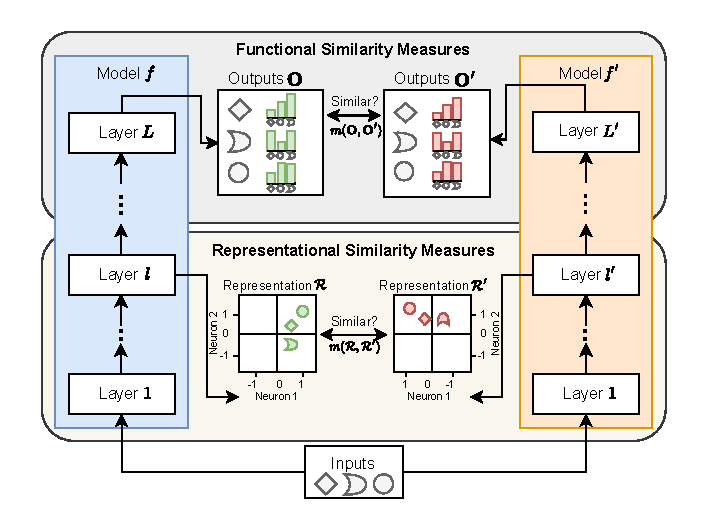
\includegraphics[width=\linewidth]{Abschlussarbeit/Pictures/Similarity90Deg.drawio.pdf}
    \caption{Visualization of representational and functional similarity \cite{klabunde_similarity_2024}.}
    \label{fig:SimilarityOfNN}
\end{figure}


        %\section{Similarity of Neural Networks}
        \section{Representational Similarity Measure}\label{RMS}
        %Within this section, we define the \textit{representational measure similarity}, that measures the difference between the activations of intermediate layers.
%Afterwards, we give an overview about representational similarity of neural networks which is determined by a similarity measure $m$. 

In order to compare neural networks, representational similarity methods typically assess how similar the internal representations of a fixed set of inputs are across different models or layers.  
We will focus in the following on comparing activations at specific layers, but alternative approaches may also consider other components, such as weights or gradients.


%In order to compare neural networks, representational similarity measurements examine how similar the activations of a fixed set of inputs at any pair of layers are.
Therefore, we consider a representation of the model $f$ at layer $l$:
\begin{equation*}
    R:=R^{(l)}=(f^{(l)} \circ f^{(l-1)} \circ ... \circ f^{(1)}) \in \mathbb{R}^{N\times D}.
\end{equation*}
Here, \( N \) denotes the (possibly infinite) number of datapoints, and \( D \) the number of neurons in a single layer.


\begin{definition}[Representational similarity measures] A representational similarity measure is a map 
\begin{equation*}
    m: \mathbb{R}^{N\times D} \times \mathbb{R}^{N\times D} \longrightarrow \mathbb{R},
\end{equation*} 
that assigns a similarity score $m(R, R')$ to a pair of representations $R,R'$ of different models $f,f'$ that use the same inputs $\mathcal{X}$.    
\end{definition}

Nevertheless, we can consider two representation matrices \( R, R' \in \mathbb{R}^{N \times D} \) to be equivalent, even if they are not identical element-wise.
This is particularly relevant when comparing language encoders whose outputs may differ due to arbitrary linear transformations, such as sign flips (e.g., \( R = -R' \)) or rotations.
Such transformations do not necessarily alter the underlying structure or information content of the representations.
Hence, comparing representations up to such equivalence classes allows us to focus on their functional behavior rather than their raw numerical values.

The specific type of transformation used to define equivalence depends on the context and intended application.  
For instance, some analyses may permit any orthogonal transformation, while others restrict equivalence to affine or even task-informed transformations.

%Nevertheless, we can consider two representation matrices $R,R'\in \mathbf{R}^{N\times D}$ to be equivalent, even if they are not identical on an element-per-element basis.
%This is the case, if we consider representations that differ in their sign i.e. $R=-R'$, or when we rotate onto another. 

By using terms of bijective mappings (transformations), we can formalize the notions of equivalence as follows:
\begin{align*}
    \psi:\mathbb{R}^{N\times D} &\to \mathbb{R}^{N\times D}\\
    \psi(R)&=R'.
\end{align*}


\begin{definition}[Equivalence of Representations]
    Let $R,R' \in\mathbb{R}^{N\times D}$ be two representations and $\mathcal{T}:=\mathcal{T}(N,D)$ a group. 
    We denote $R$ and $R'$ as equivalent with respect to a group $\mathcal{T}$, written as $R \sim_\mathcal{T}R'$ if there is a $\psi\in \mathcal{T}$, such that $\psi(R)=R'$
\end{definition}
The group of transformations under which representations should be considered equivalent is of crucial importance in practice, since equivalent representations should be indistinguishable for the chosen similarity measure.
In contrast, non-equivalent representations must be distinguishable for a similarity measure.
Formally, this means that a measure must be invariant to exactly those groups of transformations under which the underlying representations are equivalent.

%\begin{definition}[Invariant Representational Similarity Measure]
%    Let $R,R' \in\mathbb{R}^{N\times D}$ be two representations, $\mathcal{T}(N,D)$ a group and $\varphi\in \mathcal{T}(N,D), \varphi'\in \mathcal{T}(N,D)$.
%    A similarity measure $m$ is called invariant to a group of transformations $\mathcal{T}$ if it holds:
%    \[m(R,R')=m(\varphi(R),\varphi'(R)) \quad  \forall R,R' \text{ and } \forall\varphi, \varphi'\]  
%    \[\Longrightarrow m(R,R)=m(R,R') \text{ if } R \sim_\mathcal{T} R'\]
%\end{definition}

\begin{definition}[Invariant Representational Similarity Measure]
Let $\mathcal{T}(N, D)$ be a group of transformations acting on representation matrices in $\mathbb{R}^{N \times D}$.  
A similarity measure \( m: \mathbb{R}^{N \times D} \times \mathbb{R}^{N \times D} \to \mathbb{R} \) is called \emph{invariant under} \( \mathcal{T}(N, D) \) if for all \( R, R' \in \mathbb{R}^{N \times D} \) and all \( \varphi, \varphi' \in \mathcal{T}(N, D) \), it holds that
\[
    m(R, R') = m(\varphi(R), \varphi'(R')).
\]
In particular, if \( R \sim_{\mathcal{T}} R' \), then \( m(R, R) = m(R, R') \).
\end{definition}

Using this definition, we will later examine whether the similarity measures considered satisfy the axioms of a distance metric.  
In the context of representational similarity, however, one of these axioms—namely the \emph{identity of indiscernibles}, can be relaxed.  
Rather than requiring that \( m(R, R') = 0 \) if and only if \( R = R' \), it is sufficient to require that
\[
m(R, R') = 0 \iff R \sim_{\mathcal{T}} R',
\]
where \( \mathcal{T} \) is a group of transformations under which the measure \( m \) is invariant~\cite{williams_generalized_2021}.  
This allows the similarity measure to capture equivalence of representations up to transformations that preserve their functional or structural meaning.




%Using this definition, we can analyse later in the thesis, whether the measures meet the criteria of a distance metric.
%In the sense of representational similarity the criteria can be relaxed to only require $m(R,R')= 0$ if and only if $R\sim_\mathcal{T}R'$ for a group of transformations $\mathcal{T}$ that $m$ is invariant to \cite{williams_generalized_2021}.



%An instance representation $R_i=((f^{(l)} \circ f^{(l-1)} \circ ... \circ f^{(1)})(\mathbf{X_i}\in \mathbb{R}^D$ represents the activations of instances $i \in \{1,...,N\}$, which corresponds to the $i$-th row. of $R$
        \section{Functional Similarity Measure}\label{FMS}      If we measure similarity by the output behavior of neural networks, we refer to \emph{functional similarity measures}.
To formalize this, let \( f \) be a neural network trained on a set of inputs \( X = \{x_1, \ldots, x_N\} \) to perform a classification task with \( C \) output classes.
Evaluated on a subset \( Y \subseteq X \), the network produces an output matrix
\[
    \mathbf{O} := f(Y) \in \mathbb{R}^{N \times C},
\]
where \( N \) denotes the (possibly infinite) number of datapoints and \( C \) the number of classes.


\begin{definition}[Functional similarity measure]
A functional similarity measure is a map 
\begin{equation*}
    m: \mathbb{R}^{N\times D} \times \mathbb{R}^{N\times D} \longrightarrow \mathbb{R}, 
\end{equation*}
that assigns a similarity score $m(\mathbf{O}, \mathbf{O}')$ to a pair of outputs $\mathbf{O}, \mathbf{O}'$ of different models $f,f'$ that use the same inputs $X$. 

It is assumed that the compared outputs \( \mathbf{O}, \mathbf{O}' \in \mathbb{R}^{N \times C} \) are class-aligned, meaning that the columns of both matrices correspond to the same set of classes in the same order.
%It is assumed that the compared outputs $\mathbf{O},\mathbf{O}'\in\mathbb{R}^{N\times C}$ are aligned in that the columns $\mathbf{O}_{-,c}$ and $\mathbf{O}_{-,c}$ correspond to the probability score of the same class $c$.
\end{definition}

We induce an equivalence relation based on that similarity in the following.

\begin{definition}[Equivalence of Functions]
Let $X$ be a fixed input set, $f,f'$ two neural networks and $m(f(Y),f'(Y))\in \mathbb{R}$ the functional similarity score.

We denote $f$ and $f'$ as equivalent $f \sim_Y f'$, if $m(f(Y),f'(Y))\geq \tau$, where the user defined similarity threshold $\tau \to 0$.
In the following, we will write for simplicity $f=f'$ if both neural networks produce the same output as both of them are an element of the same equivalence class. 
    
\end{definition}
 
        %\section{Related Work}\label{RW}
        %Most existing approaches to neural network similarity focus on comparing representations across models under linear transformations, such as permutations, orthogonal mappings, or affine projections \cite{kornblith_similarity_2019, williams_generalized_2021, li_convergent_2016}. These methods aim to identify structural equivalence of networks trained with different initializations or data.

A more recent and relevant contribution by Chan et al.~\cite{chan_affine_2024} introduces an \emph{affine homotopy} between language encoders, modeling transformations through affine maps.
While this approach is theoretically elegant, it assumes that encoders are related through linear structure — an assumption that fails to capture the complex nonlinear relations often observed in practice.

In contrast, our work investigates \emph{nonlinear} transformations between encoders by formalizing intrinsic and extrinsic homotopies, as developed in Chapters~\ref{EA} and~\ref{ISA}. 
We interpret similarity as a generalized distance between models and provide a framework that moves beyond the limitations of linear alignment methods.

        \chapter{Similarity Analysis using Affine Transformations}\label{EA}    
        In this chapter, we present the framework developed by Chan et al.~\cite{chan_affine_2024}, which introduces two notions of homotopy to compare language encoders in a principled way.
 
 These two notions, \emph{intrinsic} and \emph{extrinsic homotopy}, capture distinct perspectives on model similarity.  
 Intrinsic homotopy focuses on representational similarity: it compares models solely based on their internal hidden representations, typically using the final encoder layer, and does not rely on any downstream task.  
 
 In contrast, extrinsic homotopy assesses models in a task-specific context. Here, a classification head is trained on top of each encoder, and similarity is measured via alignment of outputs or task performance.
 
 At the core of the intrinsic and extrinsic perspective lies a \emph{specialization quasi-ordering} induced by a hemi-metric.  
 This preorder expresses directional approximability between encoders and serves as the formal backbone for defining intrinsic and extrinsic homotopy.  
 By separating intrinsic and extrinsic views, this framework enables a comprehensive analysis of model similarity from both structural and functional perspectives.
 


Based on the Prelimiaries in Chapter~\ref{Preliminaries} a general recipe for defining hemi-metric spaces on function spaces can be defined.

\begin{definition}[Hemi-metric on Function Spaces]\label{def:Hemi_Metr_Func_Space}
Let \( X \) be a set, and let \( (Y, d) \) be a hemi-metric space. Furthermore, let 
\[
S : X \to \mathcal{P}(Y) \setminus \{ \emptyset \}, \quad x \mapsto E_x
\]
be a mapping that assigns to each \( x \in X \) a non-empty subset \( E_x \subseteq Y \).

We define a hemi-metric \( d_S^{\mathcal{H}} \) on \( X \) by setting
\[
d_S^{\mathcal{H}}(x, y) := d^{\mathcal{H}}(E_x, E_y) := \sup_{y_1 \in E_y} \inf_{x_1 \in E_x} d(x_1, y_1),
\]
which is sometimes called the Hausdorff hemi-distance from \( E_x \) to \( E_y \).

Optionally, we can symmetrize this to define an extended pseudo-metric by
\[
d^{\text{sym}}_S(x, y) := \max\big( d_S^{\mathcal{H}}(x, y),\ d_S^{\mathcal{H}}(y, x) \big).
\]
\end{definition}

We now define a notion of alignment between two encoders via a class of affine transformations. Let \( S \subset \mathrm{Aff}(V) \) be a set of affine maps acting on a vector space \( V \). For two encoders \( h, g: X \to V \), we define the \( S \)-alignment from \( g \) to \( h \) by
\[
d_S(h, g) := d_\infty^{\mathcal{H}}(h, S(g)) := \inf_{\psi \in S} \| h - \psi \circ g \|_\infty,
\]
where \( S(g) := \{ \psi \circ g \mid \psi \in S \} \).

This captures how well the encoder \( g \) can be transformed into \( h \) via elements of \( S \). 
Note that \( d_S(h, g) \) is generally asymmetric: it measures the alignment from \( g \) to \( h \), but not necessarily the other way around.

We further define the \( S \)-norm of an encoder \( h \) as
\[
\| h \|_S := d_S(0_{\mathcal{E}_V}, h),
\]
which measures how well \( h \) can be approximated by an \( S \)-transformation of the zero encoder.

\medskip

This concept of affine alignment can be seen as a special case of the construction in Definition~\ref{def:Hemi_Metr_Func_Space}, where we set \( X = Y = \mathcal{E}_V \), and use the uniform convergence hemi-metric from Subsection~\ref{ND}.









\section{Intrinsic Homotopy}\label{IH}
Chan et al.~\cite{chan_affine_2024} developed the notion of \emph{intrinsic homotopy}, which aims to compare language encoders independently of any downstream task.  
The key idea is to define similarity intrinsically, based solely on the internal representations produced by the models.  
This is formalized using the structure of a hemi-metric space and a directional relation derived from it.

A central component of this framework is the \emph{specialization quasi-ordering} \( \gtrsim_d \), introduced on a hemi-metric space \( (X, d) \) as in Definition~\ref{def:quasi-ordering}.  
It captures whether one encoder can approximate another via a structure-preserving transformation.  
Since such transformations may exist in only one direction, the relation is defined as a \emph{preorder}, i.e., it is reflexive and transitive but not necessarily symmetric.

This asymmetric relation provides a principled way to compare encoders in terms of representational similarity.  
If mutual approximability holds, i.e., both \( h \gtrsim_d g \) and \( g \gtrsim_d h \), the encoders are said to be \emph{exactly intrinsically affinely homotopic}.

In practice, intrinsic homotopy is based on the output of the final hidden layer, which aggregates semantic information and serves as the default input to downstream classifiers.  
Accordingly, this notion aligns closely with the concept of representational similarity discussed in Section~\ref{RMS}.

We begin this chapter by examining how the specialization preorder arises from the hemi-metric structure and serves as the foundation for intrinsic homotopy.

\begin{lemma}\label{lemma:quasi-ordering}
Let $(X, d)$ be a hemi-metric space, and let $\gtrsim_d$ denote the specialization quasi-ordering with respect to the open ball topology. Then, for all $x, y \in X$,
\[
x \gtrsim_d y \quad \Longleftrightarrow \quad d(x, y) = 0.
\]
\end{lemma}



\begin{proof}
\glqq$\Rightarrow $\grqq  Suppose $x \gtrsim_d y$.
Then, for all $\varepsilon > 0$, we have $y \in B(x, \varepsilon)$, which implies $d(x, y) < \varepsilon$. 
Since this holds for all $\varepsilon > 0$, we must have $d(x, y) = 0$.

\glqq$\Leftarrow$\grqq Now suppose $d(x, y) = 0$. Let $U$ be any open set containing $x$. 
By Lemma~\ref{lemma:open_balls_form_base}, there exists $\varepsilon > 0$ such that $B(x, \varepsilon) \subseteq U$.
Since $d(x, y) = 0 < \varepsilon$, it follows that $y \in B(x, \varepsilon) \subseteq U$, so $x \gtrsim_d y$.
\end{proof}


We consider two encoders \( f, g \) in the real vector space of language encoders \( \mathcal{E}_V := V^{\Sigma^*} \), and define an affine intrinsic pre-order \( \gtrsim_{\mathrm{Aff}} \) on this space.

\begin{definition}[Exact Intrinsic Affine Homotopy]
Two encoders \( h, g \in \mathcal{E}_V \) are said to be \textit{exactly intrinsically affinely homotopic}, written \( h \simeq_{\mathrm{Aff}} g \), if both \( g \gtrsim_{\mathrm{Aff}} h \) and \( h \gtrsim_{\mathrm{Aff}} g \) hold.
\end{definition}

In the original formulation, two encoders \( h, g \in \mathcal{E}_V \) are defined to be exactly intrinsically affinely homotopic if
\[
d_{\mathrm{Aff}(V)}(h, g) = 0 \quad \text{and} \quad \mathrm{rank}(h) = \mathrm{rank}(g).
\]
Chan et al.~\cite{chan_affine_2024} showed that this condition is equivalent to the ladder-based formulation presented above, which is more convenient for our purpose as it avoids the need to explicitly define \(\mathrm{rank}\).


\section{Extrinsic Homotopy}\label{EH}
Compared to intrinsic homotopy, which evaluates language encoders based on their internal structure, \emph{extrinsic homotopy} focuses on their observable behavior in downstream tasks.  
It captures \emph{functional similarity}, as discussed in Section~\ref{FMS}, by assessing how similarly two encoders perform when composed with task-specific classifiers.

Formally, two encoders \( h \) and \( g \) are considered extrinsically homotopic if they yield similar performance across all downstream tasks in which they could serve as feature extractors.  
To make this precise, each encoder is composed with affine classifiers, yielding complete prediction pipelines.  
This setup allows us to define a hemi-metric that quantifies behavioral divergence between encoders across tasks.

If this distance is zero, the encoders are said to be \emph{exactly extrinsically homotopic}.  
In practice, this notion can be approximated using a finite set of input strings and optimization techniques such as gradient descent.  
Finally, we explore how extrinsic and intrinsic homotopy relate, and how functional similarity can complement representational alignment.


Let $\Sigma$ be a finite alphabet and let $\Sigma^*$ denote the set of all finite strings over $\Sigma$, i.e., the Kleene closure of $\Sigma$.  
Let $V$ be a vector space of intermediate representations, and let $W := \mathbb{R}^C$ denote the output space for a classification task with $C$ classes.

An affine map $f: V \to W$ is given by a linear map $A \in \mathcal{L}(V, W)$ and a bias vector $b \in W$, such that
\[
f(v) = A \cdot v + b \quad \text{for all } v \in V.
\]
We denote the set of all affine maps from $V$ to $W$ by $\operatorname{Aff}(V, W)$.

We define the following sets of encoder functions:
\begin{itemize}
	\item $\mathcal{E}_V := \operatorname{Map}(\Sigma^*, V)$ – encoders mapping strings to vector representations,
	\item $\mathcal{E}_W := \operatorname{Map}(\Sigma^*, W)$ – classifiers mapping strings to class scores,
	\item $\mathcal{E}_{\Delta^{C-1}} := \operatorname{Map}(\Sigma^*, \Delta^{C-1})$ – classifiers returning probability distributions over $C$ classes.
\end{itemize}

Given an encoder $h \in \mathcal{E}_V$, we define the set of affine classifiers based on $h$ as
\[
\operatorname{Aff}_{V,W}(h) := \left\{ \psi \circ h \mid \psi \in \operatorname{Aff}(V, W) \right\} \subset \mathcal{E}_W.
\]
Applying the softmax function with inverse temperature $\lambda > 0$ yields the associated family of log-linear classifiers:
\[
\mathcal{V}_C(h) := \left\{ \operatorname{softmax}_\lambda \circ f \mid f \in \operatorname{Aff}_{V,W}(h) \right\} \subset \mathcal{E}_{\Delta^{C-1}}.
\]

Based on this construction, we define a hemi-metric that quantifies the difference between two encoders $h, g \in \mathcal{E}_V$ in terms of their downstream classification behavior:
\[
d^{\mathcal{H}}_{\mathcal{V}_C}(h, g) := \sup_{\psi \in \mathcal{V}_C(h)} \inf_{\varphi \in \mathcal{V}_C(g)} \| \psi \circ h - \varphi \circ g \|_\infty.
\]

This metric captures how differently two encoders behave when composed with affine classification heads and applied to the same string input.  
It forms the basis for the definition of \emph{extrinsic homotopy}, as introduced in the following section.


%\begin{definition}[Exact extrinsic Homotopy]
%    Two encoder $g,h\in\mathcal{E}_V$ are called \textit{exactly extrinsically homotopic}, if $d^\mathcal{H}_\mathcal{V}(V,\Delta)(h,g)=0$.
%\end{definition}
\begin{definition}[Exact Extrinsic Homotopy]
Two encoders \( g, h \in \mathcal{E}_V \) are called \emph{exactly extrinsically homotopic} if
\[
d^{\mathcal{H}}_{\mathcal{V}(V,\Delta)}(h, g) = 0.
\]
\end{definition}


Furthermore, Chan et al. \cite{chan_affine_2024} defined an extrinsic affine preorder and showed, that affine instrinsic preorder is contained in the extrinsic preorder. 
This connects the internal structure of encoders to their external behavior.

In the practical concern two language encoders are not considered over the entire $\Sigma^*$, only over a finite set of strings $X=\{x_i\}^N_{i=1}$.
Then, the encoders are considered as matrices and the notion of similarity is approximated by optimizing over the affine maps, for example by using gradient descent. 
        
        \chapter{Improving Similarity Analysis using Nonlinear Transformations}\label{ISA}
        In this chapter we formalize the mathematical methods of our novel approach.
We focus on continuous non-linear transformations instead of affine ones, as presented by Chan et al. \cite{chan_affine_2024}.
The non-linear transformations are represented by a neural network in practice, as it is one of the most used state-of-the-art approaches for non-linear transformations.
We will formalize the mathematical methods to analyse the influence of continuous non-linear transformations on the approach presented in the chapter \ref{EA}.
First, we will modify the definition of intrinsic and extrinsic homotopy. 
%Therefore, we consider the set of continuous maps, which includes the set of affine maps and the set of non-linear maps, and extend these homotopies to a set of continuous maps.
Therefore, we extend the notion of homotopy by considering the set of continuous maps, which includes both linear and non-linear functions, as long as they are continuous.
Furthermore, we define an approach, where the similarity will be measured by the models performance. 


\section{Intrinsic Homotopy on Non-linear Transformations}\label{InrinsicHomotopyonNonlinTransf}
Inspired by the framework of Chan et al.~\cite{chan_affine_2024}, we consider a space of language encoders \( \mathcal{E}_V \), viewed as a subset of the space of continuous functions from sequences \( \Sigma^* \) to a finite-dimensional vector space \( V \subset \mathbb{R}^d \), where \( \Sigma \) denotes a finite alphabet and \( \Sigma^* \) its Kleene closure.

%Inspired by the framework of Chan et al. \cite{chan_affine_2024}, we consider a space of language encoders \( \mathcal{E}_V \), viewed as a subset of the space of continuous functions from sequences \( \Sigma^* \) to a finite-dimensional vector space \( V \subset \mathbb{R}^d \). 
Equipped with the uniform norm
\[
\|h\|_\infty := \sup_{x \in \Sigma^*} |h(x)|_V,
\]
the space \( (\mathcal{E}_V, \|\cdot\|_\infty) \) becomes a complete metric space with distance \( d_\infty(h, g) := \|h - g\|_\infty \), due to the completeness of \( V \).

The goal of this section is to define an intrinsic, nonlinear notion of homotopy between language encoders.  
While Chan et al. \cite{chan_affine_2024} define such a structure using affine maps, we extend this approach to a more expressive class of transformations: namely, general nonlinear maps.  
In principle, we are interested in the full range of nonlinear structure-preserving transformations.  
However, in order to ensure that the induced distance satisfies the triangle inequality, and thus defines a valid hemi-metric, we restrict ourselves to 1-Lipschitz continuous functions.  
This technical constraint is essential in the proof of Proposition~\ref{eq:intrinsic_equation}, where we rely on the fact that 1-Lipschitz functions are closed under composition and do not increase the \( \ell^\infty \)-distance.


Intuitively, we say that an encoder \( h \) is intrinsically related to another encoder \( g \) if there exists a well-behaved transformation that maps \( g \) closely to \( h \). 
To formalize this idea, we define an asymmetric notion of distance \( d_{\mathcal{F}_{\text{Lip}_1}}(h, g) \), which quantifies how well \( h \) can be approximated by transformed versions of \( g \) under a class of admissible maps. The smaller this distance, the more intrinsically related the models are. If the distance is zero, we consider the two encoders intrinsically similar.

We now make this precise using the notion of a hemi-metric as introduced in Definition~\ref{def:Hemi_Metr_Func_Space}. 

Let \( \mathcal{F} \subset \mathcal{C}(V, V) \) denote a class of admissible transformations, where \( V \subset \mathbb{R}^d \) is a finite-dimensional vector space.  
Each transformation \( \psi \in \mathcal{F} \) maps encoder outputs from \( V \) into \( V \), and induces a new encoder \( \psi \circ g \colon \Sigma^* \to V \).

In the following, we will focus on the case where \( \mathcal{F} = \mathcal{F}_{\mathrm{Lip}_1} \), the set of 1-Lipschitz continuous functions from \( V \) to itself.


Then, for any pair of encoders \( h,  g \in \mathcal{E}_V \), we define the hemi-metric, as in Definition ~\ref{def:Hemi_Metr_Func_Space} %directed distance
\[
d_{ \mathcal{F}_{\mathrm{Lip}_1}}(h, g) := \inf_{\psi \in \mathcal{F}_{\mathrm{Lip}_1}} \| h - \psi \circ g \|_\infty,
\]
which measures how well \( h \) can be approximated by transformed versions of \( g \). 
This construction induces a preorder \( h \gtrsim_{\mathrm{Intr}} g \) on the space of encoders.
 
\begin{definition}[Intrinsic Relation]\label{eq:intrinsic_equation}
Let \( h, g \in \mathcal{E}_V \), and let \(  \mathcal{F}_{\mathrm{Lip}_1} \subset \mathcal{C}(V, V) \) be a class of admissible transformations.
We say that \( h \) is intrinsically related to \( g \), written
\[
h \gtrsim_{\mathrm{Intr}} g,
\]
if the induced distance satisfies
\[
d_{\mathcal{F}_{\text{Lip}_1}}(h, g) = \inf_{\psi \in \mathcal{F}_{\mathrm{Lip}_1}} \| h - \psi \circ g \|_\infty = 0.
\]
\end{definition}

As we need to restrict ourselves to 1-Lipschitz continuous functions, we will introduce the Lipschitz Continuty in the following.   

\begin{definition}[Lipschitz Continuity]
	A function \( \psi \colon V \to W \) between two normed vector spaces is called \emph{Lipschitz continuous} \cite{forster_analysis_2025} if there exists a constant \( L \geq 0 \) such that for all \( v_1, v_2 \in V \), we have
	\[
	\| \psi(v_1) - \psi(v_2) \|_W \leq L \cdot \| v_1 - v_2 \|_V.
	\]
	The smallest such constant \( L \) is called the \emph{Lipschitz constant} of \( \psi \). If \( L \leq 1 \), we say that \( \psi \) is \emph{1-Lipschitz}.
\end{definition}


\begin{proposition}\label{prop:complete_F_Lip}
Let \(  \mathcal{F}_{\mathrm{Lip}_1} \subset \mathcal{C}(V, V) \) denote the set of 1-Lipschitz continuous functions from \( V \) to \( W \), where \( V \) and \( W \) are finite-dimensional normed vector spaces over \( \mathbb{R} \).
Then \( \mathcal{F}_{\text{Lip}_1} \) is a closed subset of the complete metric space \( (\mathcal{C}(V, V),d_{\mathcal{F}_{\text{Lip}_1}}) \), and hence itself complete.
\end{proposition}

\begin{proof}
Let \( (\psi_n) \subset \mathcal{F}_{\text{Lip}_1} \) be a sequence that converges uniformly to some function \( \psi \in \mathcal{C}(V, V) \) with respect to the supremum norm
\[
\|\psi_n - \psi\|_\infty := \sup_{x \in V} \|\psi_n(x) - \psi(x)\|_W.
\]

We show that \( \psi \) is also 1-Lipschitz:
for any \( x, y \in V \),
\[
\|\psi(x) - \psi(y)\|_W \leq \|\psi(x) - \psi_n(x)\|_W + \|\psi_n(x) - \psi_n(y)\|_W + \|\psi_n(y) - \psi(y)\|_W.
\]
Using the triangle inequality and the fact that \( \psi_n \in \mathcal{F}_{\text{Lip}_1} \), we get
\[
\|\psi(x) - \psi(y)\|_W \leq 2\|\psi - \psi_n\|_\infty + \|x - y\|_V.
\]
Taking the limit \( n \to \infty \), the first term vanishes and we obtain
\[
\|\psi(x) - \psi(y)\|_W \leq \|x - y\|_V,
\]
so \( \psi \) is 1-Lipschitz and thus \( \psi \in \mathcal{F}_{\text{Lip}_1} \). Therefore, \( \mathcal{F}_{\text{Lip}_1} \) is closed.

Since \( (\mathcal{C}(V, V), d_\infty) \) is a complete metric space (by completeness of \( W \) \cite{werner_funktionalanalysis_2005}), it follows that \( \mathcal{F}_{\text{Lip}_1} \) is complete as a closed subset of a complete space.
\end{proof}



To formalize how well an encoder \( h \) can be approximated by another encoder \( g \) via a transformation from a given function class, we define the \emph{intrinsic approximation distance}
\[
d_{\mathcal{F}_{\text{Lip}_1}}(h, g) := \inf_{\psi \in  \mathcal{F}_{\mathrm{Lip}_1}} \| h - \psi \circ g \|_\infty,
\]
where \(\mathcal{F}_{\mathrm{Lip}_1}\subset \mathcal{C}(V, V) \) denotes a set of admissible transformations – for instance, the class of 1-Lipschitz continuous maps.
This defines a \emph{hemi-metric} on the space of encoders \( \mathcal{E}_V \), as it may fail to be symmetric.

The \emph{specialization quasi-ordering} induced by this hemi-metric is given by
\[
h \gtrsim_{ \mathcal{F}_{\mathrm{Lip}_1}} g \quad \Leftrightarrow \quad d_{\mathcal{F}_{\text{Lip}_1}}(h, g) = 0.
\]
Intuitively, this means that \( h \) can be approximated arbitrarily well by applying some transformation \( \psi \in  \mathcal{F}_{\mathrm{Lip}_1} \) to \( g \). That is, for any error tolerance \( \varepsilon > 0 \), there exists a transformation \( \psi \in \mathcal{F}_{\mathrm{Lip}_1} \) such that \( \| h - \psi \circ g \|_\infty < \varepsilon \). The relation \( \gtrsim_{ \mathcal{F}_{\mathrm{Lip}_1}} \) is thus a \emph{preorder}: it is reflexive and transitive, but not necessarily antisymmetric.

%\begin{proposition}[Intrinsic Preorder]
%Let \( \mathcal{F}_{\text{Lip}_1} \subset \mathcal{C}(V, V) \) denote the class of 1-Lipschitz continuous transformations from \( V \) to itself.
%Then the relation \( \gtrsim_{\mathrm{Intr}} \) defined by
%\[
%h \gtrsim_{\mathrm{Intr}} g \quad \Leftrightarrow \quad \inf_{\psi \in \mathcal{F}_{\text{Lip}_1}} \| h - \psi \circ g \|_\infty = 0
%\]
%is a preorder on \( \mathcal{E}_V \); that is, it is reflexive and transitive.
%\end{proposition}

\begin{proposition}[Intrinsic Preorder]
	Let \( \mathcal{F}_{\text{Lip}_1} \subset \mathcal{C}(V, V) \) denote the class of 1-Lipschitz continuous functions from \( V \) to itself, and define the map
	\[
	d_{\mathcal{F}_{\text{Lip}_1}} : \mathcal{E}_V \times \mathcal{E}_V \to \mathbb{R}, \quad (h, g) \mapsto \inf_{\psi \in \mathcal{F}_{\text{Lip}_1}} \| h - \psi \circ g \|_\infty.
	\]
	Then \( d_{\mathcal{F}_{\text{Lip}_1}} \) is a hemi-metric, and the induced specialization quasi-ordering
	\[
	h \gtrsim_{ \mathcal{F}_{\mathrm{Lip}_1}} g \quad \Longleftrightarrow \quad d_{\mathcal{F}_{\text{Lip}_1}}(h, g) = 0
	\]
	defines a preorder on \( \mathcal{E}_V \), by Lemma~\ref{lemma:quasi-ordering}.
\end{proposition}


\begin{proof}
	We verify that \(  d_{\mathcal{F}_{\mathrm{Lip}_1}} \) is a hemi-metric on \( \mathcal{E}_V \), as required by the axioms of Definition~\ref{def:hemi_metric}.
	
	\begin{itemize}
		\item[H1:]
		For any \( h \in \mathcal{E}_V \), we have \( \mathrm{id} \in  \mathcal{F}_{\mathrm{Lip}_1} \), so
		\[
		d_{ \mathcal{F}_{\mathrm{Lip}_1}}(h, h) \leq \| h - \mathrm{id} \circ h \|_\infty = 0.
		\]
		Since the infimum is non-negative, it follows that \( 	d_{ \mathcal{F}_{\mathrm{Lip}_1}}(h, h) = 0 \).
		
		\item[H2:] Let \( h, g, f \in \mathcal{E}_V \). We want to show:
		\[
			d_{ \mathcal{F}_{\mathrm{Lip}_1}}(h,f) \leq 	d_{ \mathcal{F}_{\mathrm{Lip}_1}}(h,g) + 	d_{ \mathcal{F}_{\mathrm{Lip}_1}}(g,f).
		\]
		
		Since \( \mathcal{F}_{\text{Lip}_1} \subset \mathcal{C}(V, V) \) is the set of 1-Lipschitz continuous maps acting on the complete metric space \( (\mathcal{E}_V, d_\infty) \), we can approximate the infimum arbitrarily well.
		
		That is, for any \( \varepsilon > 0 \), there exist alignments:
		\begin{itemize}
			\item \( \psi_g \in \mathcal{F}_{\text{Lip}_1} \) such that
			\[
			\| h - \psi_g(g) \|_\infty \leq 	d_{ \mathcal{F}_{\mathrm{Lip}_1}}(h, g) + \varepsilon,
			\]
			\item \( \psi_f \in \mathcal{F}_{\text{Lip}_1} \) such that
			\[
			\| g - \psi_f(f) \|_\infty \leq 	d_{ \mathcal{F}_{\mathrm{Lip}_1}}(g, f) + \varepsilon.
			\]
		\end{itemize}
		
		Such approximations exist because the infimum in \( 	d_{ \mathcal{F}_{\mathrm{Lip}_1}} \) is taken over a set of continuous functions, and \( \mathcal{E}_V \) is complete. In particular, minimizing sequences \( (\psi_n) \subset \mathcal{F}_{\text{Lip}_1} \) with \( \| h - \psi_n(g) \|_\infty \to	d_{ \mathcal{F}_{\mathrm{Lip}_1}}(h, g) \) converge (up to subsequences) to a map in \( \mathcal{F}_{\text{Lip}_1} \), so approximations up to \( \varepsilon \) are always available.
		
		Since \( \mathcal{F}_{\text{Lip}_1} \) is closed under composition (composition of 1-Lipschitz maps is again 1-Lipschitz), we can define
		\[
		\psi := \psi_g \circ \psi_f \in \mathcal{F}_{\text{Lip}_1}.
		\]
		Then
		\[
			d_{ \mathcal{F}_{\mathrm{Lip}_1}}(h, f) \leq \| h - \psi(f) \|_\infty = \| h - \psi_g(\psi_f(f)) \|_\infty.
		\]
		
		We estimate this norm using the triangle inequality:
		\[
		\| h - \psi_g(\psi_f(f)) \|_\infty 
		\leq \| h - \psi_g(g) \|_\infty + \| \psi_g(g) - \psi_g(\psi_f(f)) \|_\infty.
		\]
		
		The first term is bounded by \(	d_{\mathcal{F}_{\mathrm{Lip}_1}}(h, g) + \varepsilon \) by construction. To bound the second term, we use the fact that \( \psi_g \) is 1-Lipschitz, i.e., has Lipschitz constant \( L = 1 \):
		\[
		\| \psi_g(g) - \psi_g(\psi_f(f)) \|_\infty \leq L \cdot \| g - \psi_f(f) \|_\infty \leq 	d_{\mathcal{F}_{\mathrm{Lip}_1}}(g, f) + \varepsilon.
		\]
		
		Putting it all together:
		\[
		d_{\mathcal{F}_{\mathrm{Lip}_1}}(h, f) \leq \| h - \psi_g(g) \|_\infty + \| g - \psi_f(f) \|_\infty 
		\leq d_{\mathcal{F}_{\mathrm{Lip}_1}}(h, g) +  d_{\mathcal{F}_{\mathrm{Lip}_1}}(g, f) + 2\varepsilon.
		\]
		
		Since \( \varepsilon > 0 \) was arbitrary, the triangle inequality follows:
		\[
		 d_{\mathcal{F}_{\mathrm{Lip}_1}}(h, f) \leq  d_{\mathcal{F}_{\mathrm{Lip}_1}}(h, g) +  d_{\mathcal{F}_{\mathrm{Lip}_1}}(g, f).
		\]
		
	\end{itemize}

	
	Note that the triangle inequality in this form relies on the fact that all transformation functions in \( \mathcal{F}_{\text{Lip}_1} \) have Lipschitz constant \( L = 1 \).  
	If we allowed larger constants \( L > 1 \), the second term 
	\[
	\| \psi_g(g) - \psi_g(\psi_f(f)) \|_\infty \leq L \cdot \| g - \psi_f(f) \|_\infty
	\]
	would scale the second distance term by \(L\), and we would only obtain the weaker inequality
	\[
	 d_{\mathcal{F}_{\mathrm{Lip}_1}}(h, f) \leq  d_{\mathcal{F}_{\mathrm{Lip}_1}}(h, g) + L \cdot  d_{\mathcal{F}_{\mathrm{Lip}_1}}(g, f),
	\]
	which does not satisfy the standard triangle inequality unless \(L = 1\).  
	Hence, the restriction to 1-Lipschitz maps is essential to ensure that \(  d_{\mathcal{F}_{\mathrm{Lip}_1}} \) defines a hemi-metric.
	
	Consequently, \(  d_{\mathcal{F}_{\mathrm{Lip}_1}} \) satisfies the axioms of a hemi-metric on \( \mathcal{E}_V \) in the sense of Definition~\ref{def:hemi_metric}.
	
	To complete the proof, we verify that the relation
	\[
	h \gtrsim_{\mathrm{Intr}} g \quad \Longleftrightarrow \quad  d_{\mathcal{F}_{\mathrm{Lip}_1}}(h, g) = 0
	\]
	is a preorder on \( \mathcal{E}_V \):
	
	\begin{itemize}
		\item Reflexivity: For all \( h \in \mathcal{E}_V \), we have \(  d_{\mathcal{F}_{\mathrm{Lip}_1}}(h, h) = 0 \) by axiom (H1), so \( h \gtrsim_{\mathrm{Intr}} h \).
		\item Transitivity: Let \( h \gtrsim_{\mathrm{Intr}} g \) and \( g \gtrsim_{\mathrm{Intr}} f \), i.e., \(  d_{\mathcal{F}_{\mathrm{Lip}_1}}(h, g) = 0 \) and \(  d_{\mathcal{F}_{\mathrm{Lip}_1}}(g, f) = 0 \). Then by the triangle inequality:
		\[
		 d_{\mathcal{F}_{\mathrm{Lip}_1}}(h, f) \leq  d_{\mathcal{F}_{\mathrm{Lip}_1}}(h, g) +  d_{\mathcal{F}_{\mathrm{Lip}_1}}(g, f) = 0,
		\]
		hence \(  d_{\mathcal{F}_{\mathrm{Lip}_1}}(h, f) = 0 \), so \( h \gtrsim_{\mathrm{Intr}} f \).
	\end{itemize}
	
	Thus, \( \gtrsim_{\mathrm{Intr}} \) is reflexive and transitive, i.e., a preorder.
\end{proof}


\begin{definition}[Exact Intrinsic Non-Linear Homotopy]
Let \( h, g \in \mathcal{E}_V \), and let \( \mathcal{F}_{\text{Lip}_1} \subset \mathcal{C}(V, V) \) denote the class of admissible 1-Lipschitz continuous transformations.  
We say that \( h \) and \( g \) are \emph{exactly intrinsically non-linearly homotopic}, written
\[
h \gtrsim_{\mathcal{F}_{\text{Lip}_1}} g,
\]
if both directional distances vanish:
\[
d_{\mathcal{F}_{\text{Lip}_1}}(h, g) := \inf_{\psi \in \mathcal{F}_{\text{Lip}_1}} \| h - \psi \circ g \|_\infty = 0
\quad \text{and} \quad
d_{\mathcal{F}_{\text{Lip}_1}}(g, h) := \inf_{\phi \in \mathcal{F}_{\text{Lip}_1}} \| g - \phi \circ h \|_\infty = 0.
\]
That is, each encoder can be approximated arbitrarily well (in the \( \ell^\infty \)-norm) by applying admissible transformations to the other.
\end{definition}




\section{Extrinsic Homotopy on Non-linear Transformations}
\label{ExtrinsicHomotopyonNonlinTransf}
In this section, we extend the notion of homotopy to incorporate extrinsic structure, focusing not only on the encoder representations themselves, but also on their behavior when composed with downstream classifiers.

Whereas intrinsic homotopy compares encoder functions directly via transformations in function space, extrinsic homotopy evaluates the functional output of composite systems, such as encoder–classifier pipelines.

The key idea is to assess whether one encoder can emulate another by applying suitable post-processing transformations e.g., neural classifiers, followed by normalization.

To formalize this, let \( V \subset \mathbb{R}^d \) denote the output space of an encoder and \( W = \mathbb{R}^C \) the target space of classifier outputs (e.g., logits).
We fix a class of admissible transformations \( \mathcal{C}_{V,W} \subset \mathcal{C}(V,W) \), consisting of continuous, potentially non-linear maps that preserve relevant structure (e.g., Lipschitz continuity or smoothness). 
These transformations model classifiers applied to encoder outputs.

Let $\Sigma$ be a finite alphabet and let $\Sigma^*$ denote the set of all finite strings over $\Sigma$, i.e., the Kleene closure of $\Sigma$.  
Let $V$ be a vector space of intermediate representations, and let $W := \mathbb{R}^C$ denote the output space for a classification task with $C$ classes.

We fix a class of admissible transformations \( \mathcal{C}_{V,W} \subset \mathcal{C}(V, W) \), consisting of continuous, potentially nonlinear functions (e.g., neural networks) that map encoder representations into classifier logits. These functions model downstream classifiers.

We define the following sets of functions:
\begin{itemize}
	\item $\mathcal{E}_V := \operatorname{Map}(\Sigma^*, V)$ – encoders mapping strings to vector representations,
	\item $\mathcal{E}_W := \operatorname{Map}(\Sigma^*, W)$ – classifiers mapping strings to class scores (logits),
	\item $\mathcal{E}_{\Delta^{C-1}} := \operatorname{Map}(\Sigma^*, \Delta^{C-1})$ – classifiers returning class probability distributions.
\end{itemize}

Given an encoder $h \in \mathcal{E}_V$, we define the set of classifier functions applied to $h$ as
\[
\mathcal{C}_{V,W}(h) := \left\{ \psi \circ h \mid \psi \in \mathcal{C}_{V,W} \right\} \subset \mathcal{E}_W.
\]
Applying the softmax function with inverse temperature $\lambda > 0$ yields the associated family of nonlinear logit-to-probability classifiers:
\[
\mathcal{V}_C(h) := \left\{ \operatorname{softmax}_\lambda \circ f \mid f \in \mathcal{C}_{V,W}(h) \right\} \subset \mathcal{E}_{\Delta^{C-1}}.
\]
Here, $\operatorname{softmax}_\lambda: W \to \Delta^{C-1}$ is defined as
\[
\operatorname{softmax}_\lambda(x)_i := \frac{\exp(\lambda x_i)}{\sum_{j=1}^C \exp(\lambda x_j)} \quad \text{for } x \in \mathbb{R}^C,\; i = 1,\dots,C.
\]


This framework allows us to compare encoders extrinsically by measuring how closely the outputs of their composed pipelines align. 
Following Definition~\ref{def:Hemi_Metr_Func_Space}, we define the extrinsic hemi-metric as:
%\[
%d^{\mathcal{H}}_{\mathcal{C}_{V,W}}(h, h) := \sup_{\psi \in \mathcal{C}_{V,W}} \inf_{\varphi \in \mathcal{C}_{V,W}} \| \operatorname{softmax}_\lambda ( \psi \circ g) - \operatorname{softmax}_\lambda( \varphi \circ h )\|_\infty,
%\]
\[
d^{\mathcal{H}}_{\mathcal{C}_{V,W}}(h, g) := \sup_{\psi \in \mathcal{C}_{V,W}} \inf_{\varphi \in \mathcal{C}_{V,W}} \|  \psi \circ h - \varphi \circ g \|_\infty,
\]

which quantifies how well the output of encoder \( g \) can be aligned to that of \( h \) through admissible post-transformations in \( \mathcal{C}_{V,W} \).  


\begin{definition}[Norm-induced Distance Functions]
Using the hemi-metric framework introduced in Definition~\ref{def:Hemi_Metr_Func_Space}, we define two norm-induced distance functions on the encoder space \( \mathcal{E}_V \):

\begin{align*}
d^\mathcal{H}_{\mathcal{C}_{V,W}}(h,g) &:= d^\mathcal{H}_{\infty, W}\left( \mathcal{C}_{V,W}(h), \mathcal{C}_{V,W}(g) \right), \\
d_{\mathcal{F}_{\mathrm{Lip}_1}}^{\mathcal{H}}(h,g) &:= d^\mathcal{H}_{\infty, \Delta^{C-1}}\left( \mathcal{V}_C(h), \mathcal{V}_C(g) \right).
\end{align*}
\end{definition}
The first distance \( d^\mathcal{H}_{\mathcal{C}_{V,W}} \) compares the representations of \( h \) and \( g \) after all admissible nonlinear transformations, and quantifies how closely \( g \) can approximate \( h \) via such transformations.

The second distance \( d_{\mathcal{F}_{\mathrm{Lip}_1}}^{\mathcal{H}} \) measures how differently two encoders behave under downstream classification tasks, modeled via post-composition with a classifier followed by softmax normalization.

Both distances capture extrinsic discrepancies: the former in terms of raw feature transformations, the latter in terms of final classification behavior.


\begin{proposition}[Triangle Inequality for \( d^\mathcal{H}_{\mathcal{C}_{V,W}} \)]
Let \( h, g, f \in \mathcal{E}_V \). 
Then the following triangle inequality holds:
\[
d^\mathcal{H}_{\mathcal{C}_{V,W}}(h,f) \leq d^\mathcal{H}_{\mathcal{C}_{V,W}}(h,g) + d^\mathcal{H}_{\mathcal{C}_{V,W}}(g,f).
\]
\end{proposition}


\begin{proof}
We prove the inequality using the definition of \( d^\mathcal{H}_{\mathcal{C}_{V,W}} \) and the triangle inequality of the \( \infty \)-norm.

Let \( \epsilon > 0 \) be arbitrary.
Fix any \( \psi_h \in \mathcal{C}_{V,W} \). 

By the definition of the infimum, there exists \( \psi_g \in \mathcal{C}_{V,W} \) such that:
\[
d_{\infty,W}(\psi_h \circ h, \psi_g \circ g) \leq \inf_{\tilde{\psi}_g \in \mathcal{C}_{V,W}} d_{\infty,W}(\psi_h \circ h, \tilde{\psi}_g \circ g) + \epsilon.
\]
Likewise, for this fixed \( \psi_g \), there exists \( \psi_f \in \mathcal{C}_{V,W} \) such that:
\[
d_{\infty,W}(\psi_g \circ g, \psi_f \circ f) \leq \inf_{\tilde{\psi}_f \in \mathcal{C}_{V,W}} d_{\infty,W}(\psi_g \circ g, \tilde{\psi}_f \circ f) + \epsilon.
\]

Applying the triangle inequality of \( d_{\infty,W} \), we obtain:
\begin{align*}
d_{\infty,W}(\psi_h \circ h, \psi_f \circ f) 
&\leq d_{\infty,W}(\psi_h \circ h, \psi_g \circ g) + d_{\infty,W}(\psi_g \circ g, \psi_f \circ f) \\
&\leq \inf_{\tilde{\psi}_g \in \mathcal{C}_{V,W}} d_{\infty,W}(\psi_h \circ h, \tilde{\psi}_g \circ g) + \inf_{\tilde{\psi}_f \in \mathcal{C}_{V,W}} d_{\infty,W}(\psi_g \circ g, \tilde{\psi}_f \circ f) + 2\epsilon.
\end{align*}

Now take the infimum over \( \psi_f \) on the left-hand side and then the supremum over all \( \psi_h \in \mathcal{C}_{V,W} \) to obtain:
%\begin{align*}
%d^\mathcal{H}_{\mathcal{C}_{V,W}}(h,f) 
%&= \sup_{\psi_h \in \mathcal{C}_{V,W}} \inf_{\psi_f \in \mathcal{C}_{V,W}} d_{\infty,W}(\psi_h \circ h, \psi_f \circ f) \\
%&\leq \sup_{\psi_h \in \mathcal{C}_{V,W}} \left( \inf_{\tilde{\psi}_g \in \mathcal{C}_{V,W}} d_{\infty,W}(\psi_h \circ h, \tilde{\psi}_g \circ g) + \inf_{\tilde{\psi}_f \in \mathcal{C}_{V,W}} d_{\infty,W}(\psi_g \circ g, \tilde{\psi}_f \circ f) \right) + 2\epsilon \\
%&\leq d^\mathcal{H}_{\mathcal{C}_{V,W}}(h,g) + d^\mathcal{H}_{\mathcal{C}_{V,W}}(g,f) + %2\epsilon.
%\end{align*}

\begin{align*}
&d^\mathcal{H}_{\mathcal{C}_{V,W}}(h,f) 
= \sup_{\psi_h \in \mathcal{C}_{V,W}} \inf_{\psi_f \in \mathcal{C}_{V,W}} d_{\infty,W}(\psi_h \circ h, \psi_f \circ f) \\
&\leq \sup_{\psi_h \in \mathcal{C}_{V,W}} \left( \inf_{\tilde{\psi}_g \in \mathcal{C}_{V,W}} d_{\infty,W}(\psi_h \circ h, \tilde{\psi}_g \circ g) + \inf_{\tilde{\psi}_f \in \mathcal{C}_{V,W}} d_{\infty,W}(\tilde{\psi}_g \circ g, \tilde{\psi}_f \circ f) \right) + 2\epsilon \\
&\leq \sup_{\psi_h \in \mathcal{C}_{V,W}} \inf_{\tilde{\psi}_g \in \mathcal{C}_{V,W}} d_{\infty,W}(\psi_h \circ h, \tilde{\psi}_g \circ g) 
+ \sup_{\tilde{\psi}_g \in \mathcal{C}_{V,W}} \inf_{\tilde{\psi}_f \in \mathcal{C}_{V,W}} d_{\infty,W}(\tilde{\psi}_g \circ g, \tilde{\psi}_f \circ f) 
+ 2\epsilon \\
&= d^\mathcal{H}_{\mathcal{C}_{V,W}}(h,g) + d^\mathcal{H}_{\mathcal{C}_{V,W}}(g,f) + 2\epsilon.
\end{align*}


Since \( \epsilon > 0 \) was arbitrary, the result follows.
\end{proof}



\begin{proposition}\label{prop:softmax_lip}
The temperature-scaled softmax function
\[
\operatorname{softmax}_\lambda(z)_i := \frac{e^{\lambda z_i}}{\sum_{j=1}^n e^{\lambda z_j}}
\]
is Lipschitz continuous with respect to the $\ell^\infty$ norm with Lipschitz constant at most $\frac{\lambda}{2}$.
\end{proposition}

\begin{proof}
The softmax function is continuously differentiable, and its Jacobian matrix \\ \(J(z) \in \mathbb{R}^{n \times n}\) has entries
\[
J_{ij}(z) = \lambda \cdot s_i \cdot (\delta_{ij} - s_j),
\quad \text{where } s_i = \operatorname{softmax}_\lambda(z)_i.
\]
The row sums of the absolute values are
\[
\sum_{j=1}^n |J_{ij}(z)| = \lambda \cdot s_i \left( |1 - s_i| + \sum_{j \ne i} s_j \right)
= 2\lambda \cdot s_i(1 - s_i).
\]
The product $s_i(1 - s_i)$ is maximized at $s_i = \frac{1}{2}$, hence
\[
\sum_j |J_{ij}(z)| \le \frac{\lambda}{2} \quad \text{for all } i.
\]
Therefore, the operator norm satisfies $\|J(z)\|_\infty \le \frac{\lambda}{2}$, and the function $\operatorname{softmax}_\lambda$ is \\ $\frac{\lambda}{2}$~-Lipschitz with respect to the $\ell^\infty$ norm.
\end{proof}


%\begin{proposition}[Extrinsic Preorder]
	%Let \( \mathcal{F}_{\text{Lip}_1} \subset \mathcal{C}(V, W) \) denote the class of 1-Lipschitz continuous functions from \( V \) to itself, and define the map
	%\[
	%d_{\mathcal{F}_{\text{Lip}_1}} : \mathcal{E}_V \times \mathcal{E}_V \to \mathbb{R}, \quad (h, g) \mapsto \inf_{\psi \in \mathcal{F}_{\text{Lip}_1}} \| h - \psi \circ g \|_\infty.
	%\]
	%Then \( d_{\mathcal{F}_{\text{Lip}_1}} \) is a hemi-metric, and the induced specialization quasi-ordering
	%\[
	%h\gtrsim_{\mathcal{C}_\text{Ext}} g \quad \Longleftrightarrow \quad d_{\mathcal{F}_{\text{Lip}_1}}(h, g) = 0
	%\]
	%defines a preorder on \( \mathcal{E}_V \), by Lemma~\ref{lemma:quasi-ordering}.
%\end{proposition}


\begin{definition}[Extrinsic Relation]
	Let $h, g \in \mathcal{E}_V$. 
	We define the extrinsic relation as:
	\[
	h \gtrsim_{\mathrm{Ext}} g \quad \Leftrightarrow \quad d_{\mathcal{F}_{\mathrm{Lip}_1}}^{\mathcal{H}}(h,g) = 0.
	\]
\end{definition}

\begin{proposition}[Extrinsic Preorder]
	Let \( \mathcal{F}_{\mathrm{Lip}_1} \subset \mathcal{C}(V, W) \) denote the class of 1-Lipschitz continuous functions from \( V \) to \( W \).  
	Define the extrinsic approximation distance by
	\[
	d_{\mathcal{F}_{\mathrm{Lip}_1}}^{\mathcal{H}}(h, g) := \sup_{\psi \in \mathcal{F}_{\mathrm{Lip}_1}} \inf_{\varphi \in \mathcal{F}_{\mathrm{Lip}_1}} \| \psi \circ h - \varphi \circ g \|_\infty,
	\]
	for \( h, g \in \mathcal{E}_V \), where \( \mathcal{E}_V \subset \operatorname{Map}(\Sigma^*, V) \) is the space of encoders into \( V \).
	
	Then \( d_{\mathcal{F}_{\mathrm{Lip}_1}}^{\mathcal{H}} \) is a hemi-metric on \( \mathcal{E}_V \), and the induced relation
	\[
	h \gtrsim_{\mathrm{Ext}} g \quad \Longleftrightarrow \quad d_{\mathcal{F}_{\mathrm{Lip}_1}}^{\mathcal{H}}(h, g) = 0
	\]
	defines a preorder on \( \mathcal{E}_V \).
\end{proposition}





\begin{proof}
We show first, that $d_{\mathcal{F}_{\mathrm{Lip}_1}}^{\mathcal{H}}$ is a hemi-metric as defined in Definition~\ref{def:hemi_metric}. 
%This implies that the induced relation is a preorder.


\begin{itemize}
    \item [H1:] $d_{\mathcal{F}_{\mathrm{Lip}_1}}^{\mathcal{H}} \geq 0$.
    \item[] Since $d_{\mathcal{F}_{\mathrm{Lip}_1}}^{\mathcal{H}}$ is a metric, the Hausdorff-Hoare-map inherits non-negativity
    \item [] $d_{\mathcal{F}_{\mathrm{Lip}_1}}^{\mathcal{H}}(h,h) =  0 \quad \forall h \in \mathcal{E}_V$.
    %\item \textbf{Identity of Indiscernible} $d_{\mathcal{F}_{\mathrm{Lip}_1}}^{\mathcal{H}}(h,h) =  0 \quad \forall h \in \mathcal{E}_V$.
    \item[] For $h=g$ we have $\mathcal{C}_{V,W}(h)=\mathcal{V}(V,\Delta)(g)$ and the infimum becomes zero.
    \item [H2:] Let \( h, g, f \in \mathcal{E}_V \).
    We show that
    %\item \textbf{Triangle Inequality:} Let \( h, g, f \in \mathcal{E}_V \). We show that
    \[
    d_{\mathcal{F}_{\mathrm{Lip}_1}}^{\mathcal{H}}(h,f) \leq d_{\mathcal{F}_{\mathrm{Lip}_1}}^{\mathcal{H}}(h,g) + d_{\mathcal{F}_{\mathrm{Lip}_1}}^{\mathcal{H}}(g,f).
    \]
    To do so, consider the following setup: Let \( h \in \mathcal{E}_V \) be a language encoder \( h: \Sigma^* \to V \), and let \( \psi \in \mathcal{C}_{V,W} \) be a transformation \( \psi: V \to W \). We define the composed map
    \[ p_\psi := \operatorname{softmax}_\lambda(\psi \circ h ): \Sigma^* \to \Delta^{C-1},
    \]
    which can be interpreted as assigning probability distributions over \( C \) classes. This yields the compositional structure
    \[
    \Sigma^* \xrightarrow{h} V \xrightarrow{\psi} W \xrightarrow{\operatorname{softmax}_\lambda} \Delta^{C-1}.
    \]

   % Since \( \operatorname{softmax}_\lambda \) is a Lipschitz-continuous map with constant \( L = \frac{1}{\lambda} \), the Lipschitz property carries over to the composition with any function \( \psi \in \mathcal{C}_{V,W} \). 
    
Since Proposition~\ref{prop:softmax_lip} shows, \( \operatorname{softmax}_\lambda \colon \mathbb{R}^N \to \Delta^{N-1} \) is differentiable with bounded Jacobian entries, it is Lipschitz continuous with respect to the \( \ell^\infty \)-norm. In particular, there exists a constant \( L > 0 \) such that for all \( x, y \in \mathbb{R}^N \),
\[
\|\operatorname{softmax}_\lambda(x) - \operatorname{softmax}_\lambda(y)\|_\infty \leq L \cdot \|x - y\|_\infty.
\]
This Lipschitz continuity extends to function composition: for any \( \psi \in \mathcal{C}_{V,W} \), the composed function \( \operatorname{softmax}_\lambda( \psi) \in \mathcal{C}_{V,\Delta^{C-1}} \) satisfies
\[
\| \operatorname{softmax}_\lambda(\psi(h)) - \operatorname{softmax}_\lambda(\psi(g)) \|_\infty \leq L \cdot \| \psi(h) - \psi(g) \|_\infty.
\]

In particular, the Hausdorff–Hoare distances satisfy
\[
d_{\infty, \Delta^{C-1}}^\mathcal{H}(\operatorname{softmax}_\lambda( \mathcal{C}_{V,W}(h)), \operatorname{softmax}_\lambda (\mathcal{C}_{V,W}(g)) )
\leq L \cdot d^\mathcal{H}_{\infty, W}(\mathcal{C}_{V,W}(h), \mathcal{C}_{V,W}(g)),
\]
where the Hausdorff–Hoare distance is computed with respect to the supremums norm over \( V \) and the \( \ell^\infty \)-norm on the codomain.

As a result, the triangle inequality for \( d^\mathcal{H}_{\mathcal{C}_{V,W}} \) implies the triangle inequality for the softmax-composed version,
\[
d_{\mathcal{F}_{\mathrm{Lip}_1}}^{\mathcal{H}}(h,f) \leq d_{\mathcal{F}_{\mathrm{Lip}_1}}^{\mathcal{H}}(h,g) + d_{\mathcal{F}_{\mathrm{Lip}_1}}^{\mathcal{H}}(g,f),
\]
provided that \( L = 1 \).  
If \( L > 1 \), the inequality remains valid after rescaling the distance function accordingly.

    
%    In particular, the Hausdorff–Hoare distances satisfy:
%    \[
%    d_{\infty, \Delta^{C-1}}^\mathcal{H}(\operatorname{softmax }_\lambda( \mathcal{ C}_{V,W}(h)), \operatorname{softmax}_\lambda (\mathcal{C}_{V,W}(g)) )\leq L \cdot d^\mathcal{H}_{\infty, W}(\mathcal{C}_{V,W}(h), \mathcal{C}_{V,W}(g)).
%    \]

    %As a result, the triangle inequality for \( d^\mathcal{H}_{\mathcal{C}_{V,W}} \) implies the triangle inequality for the softmax-composed version:
    %\[
    %d_{\mathcal{F}_{\mathrm{Lip}_1}}^{\mathcal{H}}(h,f) \leq d_{\mathcal{F}_{\mathrm{Lip}_1}}^{\mathcal{H}}(h,g) + d_{\mathcal{F}_{\mathrm{Lip}_1}}^{\mathcal{H}}(g,f)
    %\]
    %provided \( \operatorname{softmax}_\lambda \) is 1-Lipschitz or the constants are appropriately absorbed.
\end{itemize}

Hence, \( d_{\mathcal{F}_{\mathrm{Lip}_1}}^{\mathcal{H}} \) is a hemi-metric.%, and the induced relation \( \gtrsim_{\mathcal{C}_\text{Ext}} \) is a preorder.

%Now define a binary relation \( \gtrsim_d \) on \( \mathcal{E}_V \) by
%\[
%h \gtrsim_d g \quad \Leftrightarrow \quad d(h, g) = 0.
%\]

We show that this relation $\gtrsim_{\mathrm{Ext}}$ is a preorder:
\begin{itemize}
    \item[]Reflexivity: For all \( h \in \mathcal{E}_V \), \( d_{\mathcal{F}_{\mathrm{Lip}_1}}^{\mathcal{H}}(h, h) = 0 \), so \( h \gtrsim_{\mathrm{Ext}} h \).
    \item[]Transitivity: If \( h \gtrsim_{\mathrm{Ext}} g \) and \( g \gtrsim_{\mathrm{Ext}} f \), then
    \[
    d_{\mathcal{F}_{\mathrm{Lip}_1}}^{\mathcal{H}}(h, f) \le d_{\mathcal{F}_{\mathrm{Lip}_1}}^{\mathcal{H}}(h, g) + d_{\mathcal{F}_{\mathrm{Lip}_1}}^{\mathcal{H}}(g, f) = 0 + 0 = 0,
    \]
    so \( h \gtrsim_{\mathrm{Ext}} f \).
\end{itemize}
Based on Lemma~\ref{lemma:quasi-ordering}, the relation \( \gtrsim_{\mathrm{Ext}} \) defined by
\[
h \gtrsim_{\mathrm{Ext}} g \quad \Longleftrightarrow \quad d_{\mathcal{F}_{\mathrm{Lip}_1}}^{\mathcal{H}}(h, g) = 0
\]
is a preorder on the encoder space \( \mathcal{E}_V \).  
This coincides with our definition of the extrinsic approximation relation \( \gtrsim_{\mathrm{Ext}} \),  
as both are defined by the vanishing of the approximation distance \( d_{\mathcal{F}_{\text{Lip}_1}} \).

\end{proof}

%\begin{definition}[Extrinsic Preorder]
%For two encoders \( h, g \in \mathcal{E}_V \), we define the relation
%\[
%h \gtrsim_{\mathcal{C}_\text{Ext}} g \quad \Leftrightarrow \quad %d_{\mathcal{F}_{\mathrm{Lip}_1}}^{\mathcal{H}}(h,g) = 0.
%\]
%\end{definition}

\begin{definition}[Exact Extrinsic Nonlinear Homotopy]
An encoder \( h \in \mathcal{E}_V \) is said to be \emph{exactly extrinsically non-linearly homotopic to} \( g \in \mathcal{E}_V \), written
\[
h \gtrsim_\text{Ext} g,
\]
if
\[
d_{\mathcal{F}_{\mathrm{Lip}_1}}^{\mathcal{H}}(h,g) = 0.
\]
\end{definition}

Note that this relation is generally not symmetric; it only expresses that \( h \) can be approximated arbitrarily well by applying admissible transformations to \( g \), not necessarily the other way around.
This directional behavior reflects the asymmetric notion of homotopy proposed in \cite{chan_affine_2024}, where similarity is understood in terms of functional approximation from one model to another.


\section{Performance-Based Similarity Measure}\label{sec:PBSM}

As explained in Chapter~\ref{SoNN}, functional similarity measures compare the outputs \( \mathbf{O}, \mathbf{O}' \in \mathbb{R}^{N\times C} \), where each element \( \mathbf{O}_{i,c} \) denotes the predicted probability or score for class \( c \) on input \( x_i \). The predicted class label is given by
\[
\hat{y}_i = \arg \max_c \mathbf{O}_{i,c}.
\]

In this work, we focus exclusively on \emph{classification agreement} as a performance-based similarity measure. This captures how often two models assign the same predicted label to the same input, independent of confidence scores or loss values.

Let \( \mathbf{O}^{(h)} \) and \( \mathbf{O}^{(g)} \) be the class score matrices of models \( h \) and \( g \), respectively. Their predicted labels are defined as
\[
\hat{y}^{(h)}_i = \arg\max_c \mathbf{O}^{(h)}_{i,c}, \quad
\hat{y}^{(g)}_i = \arg\max_c \mathbf{O}^{(g)}_{i,c}.
\]

The agreement score is then computed as
\[
\operatorname{Agreement}(h, g) = \frac{1}{N} \sum_{i=1}^N \mathds{1} \left[ \hat{y}^{(h)}_i = \hat{y}^{(g)}_i \right],
\]
where \( \mathds{1} \) denotes the indicator function.

This simple yet interpretable metric reflects functional alignment in terms of model decisions and is well suited for classification tasks.


%In this work, we focus on \emph{Spearman's rank correlation} as a performance-based similarity measure. It evaluates how well two models agree in the relative ordering of class scores for each input, regardless of the absolute values.

%\paragraph{Spearman's Rank Correlation}
%Spearman's rank correlation measures the strength and direction of a monotonic relationship between two ranked variables~\cite{sammut_encyclopedia_2017}.
%Given ranks \( x_i \) and \( y_i \) for $N$ paired observations, it is computed as:
%\[
%\rho = 1 - \frac{6 \sum_{i=1}^N (x_i - y_i)^2}{N(N^2 - 1)},
%\]
%assuming no tied ranks. In practice, ties can occur, especially with discrete prediction scores or limited numerical precision.
%In such cases, a corrected version of the Spearman correlation should be used, e.g., via Pearson correlation applied to the ranks. 
%Most statistical libraries apply these corrections automatically.

%In the context of model comparison, Spearman's correlation is computed between the class score vectors predicted by two models for each input.
%It captures the consistency in confidence structures and is especially useful when the ranking of predictions matters more than their absolute magnitude.

    \chapter{Practical Realization and Implementation}\label{sec:PRaI}
    This chapter discusses the practical implementation of the theoretically formalized approaches from Chapter~\ref{ISA}.
Since we are dealing with a non-linear and non-convex bi-level structure, it is not possible to solve the optimization with classical methods.
Instead, an iterative approach is employed: the lower-level problem is addressed via a neural network, while the upper-level problem is handled through implicit optimization and adaptation of the training process.

To ensure computational efficiency, especially in view of the large number of datasets, random seeds, and model comparisons, all core components of the experimental pipeline for intrinsic and extrinsic homotopy were implemented in \texttt{Python} and parallelized using Python's \texttt{multiprocessing} library. 
In particular, this parallelization was applied to the computation of similarity measures, the training of transformation networks, and the evaluation across tasks and model configurations.


In the following, we give an overview about the implementation that focuses on how models are loaded, processed, and evaluated for intrinsic, extrinsic and performance-based similarity.



             \section{Implementation of Loading the Models}
         %Transformer-based language models such as \texttt{BERT}, \texttt{RoBERTa}, or \texttt{ELECTRA} process text by passing token embeddings through multiple layers of self-attention and feedforward operations.
%At each layer, the model computes intermediate representations for each input token.
%These internal activations are referred to as \emph{hidden states}.
%Formally, if the input to the model is a tokenized sentence \( x = (x_1, \dots, x_n) \), the model produces for each layer \( \ell \) a sequence of vectors \( h^{(\ell)} = (h_1^{(\ell)}, \dots, h_n^{(\ell)}) \in \mathbb{R}^{n \times d} \), where \( d \) is the hidden size of the model.
Transformer-based language models such as \texttt{BERT}, \texttt{RoBERTa}, or \texttt{ELECTRA} process text by passing token embeddings through multiple layers of self-attention and feedforward operations.  
At each layer, the model computes intermediate representations for each input token, referred to as \emph{hidden states}, which encode increasingly abstract and contextualized information.

Formally, let \( x = (x_1, \dots, x_n) \) be a tokenized input sequence of length \( n \).  
For a given pretrained language model \( g \), the hidden states at layer \( \ell \) are denoted by
\[
h^{(g,\ell)}(x) = \left(h^{(g,\ell)}_1, \dots, h^{(g,\ell)}_n\right) \in \mathbb{R}^{n \times d},
\]
where \( h^{(g,\ell)}_i \in \mathbb{R}^d \) is the representation of token \( x_i \), and \( d \) is the hidden size of the model.

To obtain a fixed-size vector representation per input and layer, we compute the mean over all tokens.
This aggregation yields a fixed-size representation that enables model comparisons and downstream processing independent of input length.
\[
h^{(g,\ell)} := \frac{1}{n} \sum_{i=1}^n h_i^{(g,\ell)} \in \mathbb{R}^d.
\]
For notational convenience, we write \( h^{(g)}(x) \) when the layer \( \ell \) is fixed or clear from context.

To compute both extrinsic and intrinsic homotopy distances between different language encoders, we learn a nonlinear transformation between their internal representations.

Concretely, we train neural networks that map the hidden representations of one language model to those of another.
Let \( h \in \mathbb{R}^{d} \) denote a mean-aggregated hidden representation extracted from a pretrained language encoder for a given input from a \ac{GLUE} task, which is described in detail in Section~\ref{sec:Exp_Setup}.
Let \( \psi: \mathbb{R}^{d} \rightarrow \mathbb{R}^{d'} \) be a neural network that learns to transform these representations into the feature space of another encoder.

Unless stated otherwise, we extract hidden states from the final Transformer layer, as it typically contains the most task-relevant and semantically rich information.

During training, we treat the hidden states of the source model as inputs and the corresponding hidden states of the target model (for the same textual input) as targets.
That is, we train \( \psi \) such that
\[
\psi(h^{(g)}(x)) \approx h^{(f)}(x),
\]
where \( h^{(g)}(x) \) and \( h^{(f)}(x) \) denote the mean-aggregated hidden states produced by models \( g \) and \( f \), respectively, for the same input \( x \).

This approach enables a learned alignment between the internal representation spaces of two encoders.
Once trained, the transformation \( \psi \) allows us to compare model representations across the \ac{GLUE} tasks in terms of homotopy distances.
The composition \( \psi \circ h^{(g)} \) thus maps raw input text into the representation space of model \( f \) via a nonlinear transformation that approximates \( h^{(f)} \).
This composition forms the foundation for the extrinsic and intrinsic homotopy metrics introduced in Sections~\ref{InrinsicHomotopyonNonlinTransf} and~\ref{ExtrinsicHomotopyonNonlinTransf}.

The following implementation extracts and stores hidden states from \texttt{MultiBERTs}, \texttt{RoBERTa} and \texttt{ELECTRA}  models.

The \texttt{MultiBERTs} models differ only in their random initialization and are therefore processed individually.
All models are publicly available via Hugging Face and pretrained.
They are subsequently fine-tuned on classification tasks from the \ac{GLUE} benchmark.


To analyze the internal behavior of these models, we first extract the hidden states from all transformer layers for each input sample across several \ac{GLUE} tasks. This involves loading the respective model (\texttt{RoBERTa}, \texttt{ELECTRA}, or \texttt{MultiBERTs}), preparing the task-specific input data, and performing a forward pass to compute the hidden representations.

For each layer, the outputs are averaged across the token dimension to yield a fixed-size vector for each input. These representations, together with their associated labels, are saved for the training, validation, and test splits of the GLUE tasks.
Although the classification heads of the models are customized with additional non-linear layers to increase expressiveness, our analysis focuses on the pre-classification activations, i.e., the internal representations learned by the transformer encoder itself.

The general procedure used for extracting and saving the hidden states is summarized in Algorithm~\ref{alg:hiddenStateExtractAbstract}.


\begin{algorithm}[H]
\caption{Extraction of Hidden States and Labels for GLUE Tasks}
\label{alg:hiddenStateExtractAbstract}
\begin{algorithmic}[htb]
\Procedure{ExtractHiddenStates}{$\text{model}, \mathcal{L}$}
  \State $H, Y \gets$ empty list
  \For{$\text{batch} \in \mathcal{L}$}
    \State Move $\text{batch}$ to device (CPU/GPU)
    \State $y \gets \text{batch.labels}$
    \State $\text{batch.labels} \gets \mathbf{0}$ \Comment{Dummy labels for forward pass}
    \State $\hat{h} \gets \text{model}(\text{batch}, \text{output\_hidden\_states}=\text{True})$
    \State $h \gets \text{mean\_pool}(\hat{h}.\text{hidden\_states})$ \Comment{Mean pooling over tokens (per layer)}
    \State $H.\text{append}(h)$,\quad $Y.\text{append}(y)$
  \EndFor
  \State $H \gets \text{concatenate}(H, \text{axis}=0)$ \Comment{Stack over batch dimension}
  \State $Y \gets \text{concatenate}(Y)$
  \State \Return $H, Y$
\EndProcedure
\end{algorithmic}
\end{algorithm}

All transformer models used in this work consist of 12 layers in the encoder stack, followed by a task-specific classification head (the 13\textsuperscript{th} layer). 
These models are fully fine-tuned and downloaded in their task-specific form via Hugging Face, meaning that both the encoder and the classification head are adapted to the downstream \ac{GLUE} task.



After extracting the hidden representations for all training, validation, and test samples, we serialize the resulting tensors using PyTorch's built-in \texttt{torch.save} function. 
This enables efficient reuse of the representations in downstream tasks such as classification or similarity analysis.

The extraction and serialization process is repeated for each combination of model type (e.g., \texttt{BERT}, \texttt{RoBERTa}), random seed (in the case of \texttt{MultiBERTs}), and \ac{GLUE} task (e.g., SST-2, MNLI).

The corresponding script is fully configurable via command line arguments and supports features such as caching, adjustable batch sizes, and dynamic model selection.


         \newpage
         \section{Practical Approximation of Intrinsic Homotopy}
        In Chapter~\ref{ISA}, we extended the concept of intrinsic homotopy to a family of non-linear models and transformations.  
In this context, we consider the distance map between two language encoders \( g, h \in \mathcal{E}_V \) defined in Definition ~\ref{eq:intrinsic_equation} as
\[
d_{\mathcal{F}_{\mathrm{Lip}_1}}(h, g) = \inf_{\psi \in \mathcal{F}_{\mathrm{Lip}_1}} \|h - \psi(g)\|_\infty,
\]
where \( \mathcal{F}_{\mathrm{Lip}_1} \subset \mathcal{C}_{V,W} \) denotes a subset of continuous functions, restricted in our case to non-linear neural networks.

Building on the theoretical considerations in Section~\ref{InrinsicHomotopyonNonlinTransf} and following the affine setting analyzed by Chan et al.~\cite{chan_affine_2024}, we constrain our analysis to \emph{non-linear 1-Lipschitz continuous neural networks}.  
This restriction ensures functional comparability and regularity of the learned transformations. The transformation \( \psi \in \mathcal{F}_{\mathrm{Lip}_1} \) is thus implemented as a neural network with architectural constraints that tries to enforce the Lipschitz property.

This setup allows us to compare encoder representations \( g(x) \) and \( h(x) \) by asking whether one can be mapped into the other in a structure-preserving way.  
If such a mapping exists in both directions (i.e., \( h \approx \psi(g) \) and \( g \approx \psi^{-1}(h) \)), we refer to \( g \) and \( h \) as \emph{exactly intrinsically affinely homotopic}.

Importantly, this notion of similarity is defined independently of any particular downstream task. Therefore, we analyze the final hidden layer representation of each language encoder, as it captures the model's abstract understanding before task-specific heads are applied.

\paragraph{Model Architecture.}
To estimate the intrinsic homotopy distance, we train transformation models that map representations from one encoder space into another. For each pair of encoders \( g \) and \( h \), we learn a mapping \( \psi \) such that
\[
\psi(g(x)) \approx h(x).
\]
We consider two types of transformation models:
\begin{itemize}
    \item a linear mapping (\texttt{LinearMap}), replicating the affine baseline from Chan et al.~\cite{chan_affine_2024} and
    \item a non-linear neural network (\texttt{NonLinearNetwork}) composed of fully-connected (dense) layers with ReLU activations. 
    Each layer is equipped with spectral normalization to ensure a controlled Lipschitz constant (i.e., \( \leq 1 \)).
\end{itemize}
This architectural flexibility enables controlled comparisons between linear and non-linear function classes under Lipschitz constraints.

\paragraph{Data Handling and Model Input.}
Each transformation model operates on precomputed hidden state representations \( g(x) \) and \( h(x) \), extracted from the final encoder layer for each input sample.  
These representations are stored on disk and loaded via \texttt{DataLoader} objects during training and evaluation.  
Training is supervised using the Huber loss.

\paragraph{Training Procedure.}
Models are trained using the Adam optimizer, as shown in Listing~\ref{lst:train-func} with early stopping based on validation loss.  
Training is performed on the same predefined training split that was previously used for extracting hidden representations, with the corresponding validation split used to monitor convergence.  
We explore multiple learning rates and record the corresponding loss trajectories.  
To ensure reproducibility across random seeds and tasks, all training runs are logged using process-specific log files.


\paragraph{Evaluation.}
As defined in Section~\ref{ISA}, the intrinsic homotopy distance is the infimum of the \( \ell^\infty \)-norm between \( h(x) \) and \( \psi(g(x)) \) over all admissible transformations \( \psi \in \mathcal{F}_{\mathrm{Lip}_1} \subset \mathcal{C}_{V,W} \).  
After training, the learned transformation \( \psi^* \) approximates this infimum within the class of nonlinear 1-Lipschitz neural networks.

To evaluate the quality of this approximation, we compute the maximum deviation between the transformed and target representations over a held-out test set:
\[
\max_{x \in \mathcal{D}_{\mathrm{test}}} \| h(x) - \psi^*(g(x)) \|_\infty.
\]
This value serves as a practical estimate of the intrinsic homotopy distance.

In addition, we compute the Pearson and Spearman correlation coefficient between the transformed and target representations over the test set.  
These metrics capture whether the transformation \( \psi^* \) preserves linear or monotonic structure between the input and output representations:
\begin{itemize}
	\item The \emph{Pearson correlation coefficient} measures the linear correlation between components of \( h(x) \) and \( \psi^*(g(x)) \).
	\item The \emph{Spearman rank correlation} captures the strength of any monotonic (not necessarily linear) relationship between the two vectors.
\end{itemize}
High correlation values indicate that \( \psi^* \) not only minimizes pointwise distances but also aligns structural trends in the representation space.

Formally, the \emph{Pearson correlation coefficient} between the target and predicted representations is defined as
\[
\rho_{\mathrm{Pearson}} = \frac{\operatorname{Cov}(h(x), \psi^*(g(x)))}{\sigma_{h(x)} \, \sigma_{\psi^*(g(x))}},
\]
where \( \operatorname{Cov}(\cdot, \cdot) \) denotes the empirical covariance and \( \sigma \) the standard deviation computed over the test set.

The \emph{Spearman rank correlation} is defined analogously, but computed on the rank-transformed data:
\[
\rho_{\mathrm{Spearman}} = \rho_{\mathrm{Pearson}}(\operatorname{rank}(h(x)), \operatorname{rank}(\psi^*(g(x)))).
\]



\begin{lstlisting}[language=Python, caption={Computation of $\|h(x) - \psi(g(x))\|_\infty$ in PyTorch}, label={lst:linf-computation}]
with torch.no_grad():
    for g_batch, h_batch in test_dataloader:
        output = model(g_batch)
        diff = h_batch - output
        dist = torch.max(torch.abs(diff)) # ||h - \psi(g)||_\infty
        all_dist.append(dist.item())
\end{lstlisting}

The maximum deviation across all batches is then used as an estimate for the distance:
\begin{lstlisting}[language=Python]
overall_max = max(all_dist)
\end{lstlisting}

This value corresponds to the right-hand side of Definition~\ref{eq:intrinsic_equation}, and serves as an empirical approximation to the intrinsic homotopy distance \( d_{\mathcal{F}_{\mathrm{Lip}_1}}(g, h) \).

In addition, we compute the following metrics to enable a quantitative comparison between linear and non-linear transformations (see Section~\ref{exp:IntrinsicHOm} for detailed analysis):

\begin{itemize}
    \item the Spearman rank correlation between predicted and target representations,
    \item the Pearson correlation between input and output representations (averaged over all features),
    \item an upper bound on the Lipschitz constant via the product of spectral norms of the network's weight matrices,
    %\item a lower bound estimate using Monte Carlo sampling of Jacobians on random Gaussian input vectors.
\end{itemize}

All hyperparameters, including learning rate, number of epochs, batch size, and network type, are configurable via command-line arguments. 
Results are stored in structured directories, and summary metrics are exported in JSON format for subsequent analysis.

         \section{Practical Approximation of Extrinsic Homotopy}
         In Chapter~\ref{ISA}, we extended the concept of extrinsic homotopy to a family of non-linear models and transformations.  
In this setting, we aim to quantify the dissimilarity between two language encoders \( g, h \in \mathcal{E}_V \) by approximating the Hausdorff–Hoare distance:
\[
	d_{\mathcal{F}_{\mathrm{Lip}_1}}^{\mathcal{H}}(g, h) = \sup_{\psi \in \mathcal{C}_{V,W}} \inf_{\varphi \in \mathcal{C}_{V,W}} \|\psi\circ h - \varphi \circ g\|_\infty.
\]
Following Section~\ref{ExtrinsicHomotopyonNonlinTransf}, we restrict the hypothesis space \( \mathcal{C}_{V,W} \) to the subclass \( \mathcal{F}_{\text{Lip}_1} \subset \mathcal{C}_{V,W} \) of non-linear 1-Lipschitz continuous neural networks.  
This choice, motivated by prior work in the affine case~\cite{chan_affine_2024}, ensures bounded sensitivity and comparability across models.

Since the resulting minimax problem is non-linear and non-convex, no global optimum can be guaranteed in practice.  
Inspired by adversarial training strategies in generative models~\cite{goodfellow_generative_2014}, we approximate the solution via alternating optimization.

\paragraph{Adversarial Optimization Scheme.}
Let \( \psi, \varphi \in \mathcal{F}_{\text{Lip}_1} \) denote two neural networks modeling the transformations of the source and target encoders, respectively.  
We employ the following alternating training strategy:
\begin{itemize}
    \item In the \emph{inner loop}, we fix \( \psi \) and train \( \varphi \) to minimize the discrepancy \( \|\psi(h(x)) - \varphi(g(x))\|_\infty \).
    \item In the \emph{outer loop}, we fix \( \psi \) and update \( \varphi \) via gradient ascent to increase the discrepancy to the current approximation \( \psi(g(x)) \).
\end{itemize}
This approach mirrors the generator–discriminator dynamics in GAN training, where alternating updates push the system toward an equilibrium.  
An overview is given in Algorithm~\ref{alg:alternating-training}.

\begin{algorithm}[H]
\caption{Alternating Training of Neural Networks \(\psi\) and \(\varphi\)}
\label{alg:alternating-training}
\begin{algorithmic}[1]
\State Initialize neural networks \(\psi\), \(\varphi\), and their optimizers
\For{each training epoch}
    \For{each batch index \(i\), and inputs \(x_g, x_h\)}
        \If{\(i \bmod 2 = 0\)} \Comment{Even batch: train \(\psi\)}
            \State \(\hat{y}_\psi \gets \psi(x_g)\)
            \State \(y_\varphi \gets \varphi(x_h).\text{detach()}\)
            \State \(\mathcal{L}_\psi \gets \text{MSE}(\hat{y}_\psi, y_\varphi)\)
            \State Perform gradient \textbf{ascent} on \(-\mathcal{L}_\psi\)
        \Else \Comment{Odd batch: train \(\varphi\)}
            \State \(\hat{y}_\varphi \gets \varphi(x_h)\)
            \State \(y_\psi \gets \psi(x_g).\text{detach()}\)
            \State \(\mathcal{L}_\varphi \gets \text{MSE}(\hat{y}_\varphi, y_\psi)\)
            \State Perform gradient \textbf{descent} on \(\mathcal{L}_\varphi\)
        \EndIf
    \EndFor
\EndFor
\end{algorithmic}
\end{algorithm}

\paragraph{Model Architecture and Training.}
Both \( \psi \) and \( \varphi \) are implemented as fully connected neural networks with spectral normalization applied to all linear layers to enforce 1-Lipschitz continuity.  
Training is conducted using the Adam optimizer with early stopping based on validation loss.  
Alternating updates are controlled via mini-batch indices: even-numbered batches update \( \psi \), odd-numbered batches update \( \varphi \).  
To avoid gradient leakage between updates, we detach the target model’s output using \texttt{.detach()} during each step.

\paragraph{Evaluation.}
After training, the extrinsic homotopy distance is approximated by the maximum deviation between the transformed outputs:
\[
d^\mathcal{H}_{\mathcal{F}_{\text{Lip}_1}}(g, h) \approx \max_{x \in \mathcal{D}_{\mathrm{test}}} \| \psi(h(x)) - \varphi(g(x)) \|_\infty.
\]
This value is computed over the test set using \texttt{torch.max(torch.abs(...))} (see Listing~\ref{lst:linf-computation}).  
It serves as a practical estimate of the extrinsic homotopy distance under the considered model class \( \mathcal{F}_{\text{Lip}_1} \).

\paragraph{Additional Metrics.}
As in the previous subsection, we provide a more comprehensive view of representational alignment and to enable comparisons between extrinsic homotopy similarity and performance similarity in the following experimet in Section~\ref{exp:ExtrinsicHom}, we additionally compute:
\begin{itemize}
    \item Spearman rank correlation between \( \psi(h(x)) \) and \( \varphi(g(x)) \),
    \item Pearson correlation (averaged over dimensions),
    \item Upper bound on the Lipschitz constant via the product of spectral norms.
    %\item a Monte Carlo estimate of the Lipschitz lower bound using Jacobian norms on sampled inputs.
\end{itemize}


         
\section{Estimation of the Lipschitz Constant}

%In the proofs of the triangle inequality in chapter \ref{ISA} we had to make the requirement of lipschitz continuity.
%Therefore, it is necessary, to confirm the lipschitz continuity of the trained neural networks. 
%As we defined neural networks as complex composition of multiple layers, that create a map between input and outputs, we can only evaluate the functions value of a neural network.
%G.R. Wood and B.P. Zhang represented in their paper \cite{lipschitz_estimation} an approach, by finding the supremum of all slopes $\frac{|g(x)-g(y)|}{|x-y|}$ for distinct points $x$ and $y$ in the domain $g$, where $g$ denotes in the following the trained neural network.
%The random variable $\frac{|g(X)-g(Y)|}{|X-Y|}$ itself has a cumulative distribution function $F$, which we refer to as the slope distribution of $g$, if we sample $X$ and $Y$ uniformly from the domain.
%Then, the required Lipschitz constant is equal to the upper bound of its support. 

In the proofs of the triangle inequality in Chapter~\ref{ISA}, we required the Lipschitz continuity of the neural networks involved. Therefore, it is necessary to confirm that the trained neural networks are indeed Lipschitz continuous.

Since neural networks are defined as compositions of multiple layers that map inputs to outputs, we cannot evaluate their Lipschitz continuity analytically in general, but only approximate or bound it. In the following, we consider both upper and lower bounds on the Lipschitz constant, based on the work by Geuchen et al.~\cite{geuchen_upper_2024}.

In Section~\ref{NN}, we defined neural networks as compositions of the form
\[
\psi = f^{(L)} \circ f^{(L-1)} \circ \dots \circ f^{(0)},
\]
where each layer is given by \( f^{(i)}(x) = \sigma(W_i x + b_i) \), and the activation functions \( \sigma \) are assumed to be Lipschitz continuous. 
In particular, ReLU networks are Lipschitz continuous as compositions of Lipschitz continuous functions.

Let \( \psi \in \mathcal{C}_{V,W} \) be a neural network that maps between two language encoders, and let \( x, y \in V \). Denote the Lipschitz constant of each layer \( f^{(i)} \) by \( L_i \). By recursively applying the definition of Lipschitz continuity, we obtain the following upper bound:
\[
\|\psi(x) - \psi(y)\| \leq L_L \cdot L_{L-1} \cdots L_0 \cdot \|x - y\|.
\]
Hence, the product of the individual layer constants provides an upper bound on the global Lipschitz constant of the network.

To obtain a lower bound, we consider the basic definition of the Lipschitz constant \( L \) for a function \( \psi \in \mathcal{C}_{V,W} \):
\[
\|\psi(x) - \psi(y)\| \leq L \|x - y\| \quad \Longleftrightarrow \quad \frac{\|\psi(x) - \psi(y)\|}{\|x - y\|} \leq L.
\]
Taking the supremum over all \( x \neq y \) yields:
\[
\sup_{x \neq y} \frac{\|\psi(x) - \psi(y)\|}{\|x - y\|} \leq L.
\]

If \( \psi \) is differentiable, the local Lipschitz behavior around a point \( x \) is governed by the Jacobian \( J_\psi(x) \). The operator norm of the Jacobian gives a local estimate of the Lipschitz constant:
\[
\lim_{\|h\| \to 0} \frac{\|\psi(x + h) - \psi(x)\|}{\|h\|} = \|J_\psi(x)\|.
\]

In the case of the Euclidean norm, the induced operator norm is the spectral norm, defined as the largest singular value of the Jacobian:
\[
\|J_\psi(x)\|_2 = \sup_{\|v\| = 1} \|J_\psi(x)v\|_2.
\]
Consequently,
\[
\sup_x \|J_\psi(x)\|_2 \leq L,
\]
which provides a lower bound on the global Lipschitz constant \( L \).

In practice, computing a tight lower bound on the Lipschitz constant via the spectral norm of the Jacobian over the entire domain is computationally expensive, especially in high-dimensional settings.

An alternative approach for estimating the Lipschitz constant is presented by Wood et al.~\cite{lipschitz_estimation}.
The key idea is to approximate the supremum of all slopes
\[
\frac{\|g(x)-g(y)\|}{\|x - y\|},
\]
for distinct points \( x, y \) in the domain of the function \( g \), where \( g \) denotes the trained neural network. 
The quantity
\[
\frac{\|g(X) - g(Y)\|}{\|X - Y\|}
\]
can be interpreted as a random variable when \( X \) and \( Y \) are sampled uniformly from the domain. 
This induces a cumulative distribution function \( F \), which we refer to as the \emph{slope distribution} of \( g \).
The Lipschitz constant is then equal to the supremum of the support of \( F \).

To approximate this distribution, one repeatedly samples pairs \( (X, Y) \) from the domain and computes the corresponding slopes.
By accumulating these values and computing their maximum over many repetitions, an empirical estimate of the Lipschitz constant is obtained.

However, in our setting, this method turned out to be computationally expensive and yielded unrealistically small estimates.
This is due to the fact that the model's predictions tend to be relatively flat across large regions of the input space, which causes the majority of sampled slopes to underestimate the true Lipschitz constant. 
As a result, these empirical estimates were not informative, and we therefore rely solely on the analytically computable upper bound as a conservative estimate.


As such, we restrict ourselves to estimate an upper bound based on the product of the layer wise Lipschitz constant, which is easy to compute and provides a guaranteed over-approximation of the true Lipschitz constant. 
However, this upper bound can be quite loose in practice and should be interpreted as a worst-case estimate rather than a tight characterization of the network's sensitivity. 
%We define as G.R. Wood and B.P. Zhang  \cite{lipschitz_estimation} the upper bound for a ReLu layer as:
%\[L(\psi)\leq\sup_{x\in\mathbb{R}^d}\|A^{(L)}D^{(L-1)}(x)W^{(L-1)}...D^{(0)}(x)W^{(0)}\|,\] where $A^{(L)}$ denote the weights matrice, which contains the learned parameters of each fully connected layer and $D^{(L-1)}$ denotes the derivative of the ReLU activation at a given input $x$, it selects which neurons are active at layer $L$ for input $x$ and zeros out the others.


%an approach which we will use to get an estimation of the Lipschitz constant of the trained neural networks.
%By finding the supreme of all slopes $\frac{|g(x)-g(y)|}{|x-y|}$ for distinct points $x$ and $y$ in the domain $g$, where $g$ denotes in the following the trained neural network, the Constant can be estimated.
%The random variable $\frac{|g(X)-g(Y)|}{|X-Y|}$ itself has a cumulative distribution function $F$, which we refer to as the slope distribution of $g$, if we sample $X$ and $Y$ uniformly from the domain.
%Then, the required Lipschitz constant is equal to the upper bound of its support. 
%To receive the cumulative distribution function $F$, we sample the slopes within an interval $I$ in the reals and calculate the the maximum slope.
%This process is repeated many times.
%If we do so, the cumulative distribution of this slopes absolute values converges to the cumulative slope distribution $F$.
%If we take a random simple size $n$ from this distribution and the largest of the absolute slopes, denoted by $l$, the cumulative distribution function of $l$ will be $F^n(x)$.
%If we know the distribution to which $F$ tends with increasing $n$, we may use the estimated local parameter $L$ as an estimation of the Lipschitz constant of $g$.
%To realize this process in practice we use the following algorithm \ref{alg:LipschitzEst}. 
%\begin{algorithm}[H]
%	\caption{Estimate Lipschitz Constant via Slope Sampling}
%	\begin{algorithmic}[htbp]\label{alg:LipschitzEst}
%		\State \textbf{Input:} 
%		\State \quad Models $\mathcal{M} = \{\text{trained transformation models}\}$  
%		\State \quad Input domain interval $[a, b]$  
%		\State \quad Proximity threshold $\delta$  
%		\State \quad Number of slope samples $n$  
%		\State \quad Number of max slope repetitions $m$
%		\State \textbf{Output:} Estimated Lipschitz constant $\hat{L}$
%		
%		\Procedure{Main}{}
%		\For{model name $g_{\text{name}} \in \mathcal{M}$}
%		\State $g \gets \text{load\_model}(g_{\text{name}})$
%		\State $\hat{L}, (\text{shape}, \text{scale}) \gets \textsc{LipschitzConstant}(g, a, b, \delta, n, m)$
%		\EndFor
%		\EndProcedure
%		
%		\Function{LipschitzConstant}{$g, a, b, \delta, n, m$}
%		\State $L_{\text{values}} \gets [\,]$ \Comment List to store $m$ maximum slope values
%		\For{$i = 1$ to $m$}
%		\State $slopes \gets [\,]$
%		\For{$j = 1$ to $n$}
%		\State Sample $x \in \mathbb{R}^d$ uniformly from $[a, b]^d$
%		
%		\State Sample direction $v \sim \mathcal{N}(0, I_d)$ and normalize: $v \gets v / \|v\|$
%		\State $y \gets x + \delta \cdot v$
%		\State $g_x \gets g(x)$
%		\State $g_y \gets g(y)$
%		\State $slope \gets \frac{|g_x - g_y|}{|x - y|}$
%		\State $slopes.\text{append}(slope)$
%		\EndFor
%		\State $L_{\text{values}}.\text{append}(\max(\text{slopes}))$
%		\EndFor
%		\State $(\text{shape}, \text{loc}, \text{scale}) \gets \text{fit\_reverse\_weibull}(L_{\text{values}})$
%		\State \textbf{return} $\text{loc}, (\text{shape}, \text{scale})$
%		\EndFunction
%	\end{algorithmic}
%\end{algorithm}

         
        \section{Implementation of Performance-Based Functional- Similarity Measure}
         %To analyze the performance-based similarity measure (see Section~\ref{sec:PBSM}), we first train each language encoder on a nonlinear classification task. 
%Specifically, we use a neural network as described in Listing~\ref{lst:train-func}, which takes as input the hidden state representations produced by the language encoder and their corresponding class labels.
%These hidden states and labels are obtained by processing the dataset through the respective encoder.
%During training, we record both the predicted outputs and the ground truth labels in order to evaluate the classification performance.
%After training, we compare the performance of all models on the same classification task to assess their similarity
To analyze the performance-based similarity measure (see Section~\ref{sec:PBSM}), we evaluate how well different language encoders support nonlinear classification tasks. 
The goal is to assess how informative the internal representations of each model are for downstream prediction.

To this end, we train a neural classifier on top of the hidden state representations produced by each encoder. 
The architecture of the classifier is shown in Listing~\ref{lst:train-func}.
It takes as input the fixed-size hidden representations as represented in Algorithm ~\ref{alg:hiddenStateExtractAbstract} (obtained via mean pooling or another aggregation strategy) and the corresponding class labels.

These hidden representations and labels are obtained by running the input data through the respective language encoder. 
During training, we record the predicted class outputs and compare them to the ground-truth labels using standard classification metrics, such as accuracy and Spearman rank correlation.

Once the classifier is trained for each model, we evaluate its performance on a held-out test set.
By comparing the classification performance across models on the same task, we obtain a coarse-grained similarity signal: if two models achieve similar performance, their internal representations may be considered functionally similar from a task-oriented perspective.

To refine this view, we additionally compare the actual predictions made by the classifiers.
Specifically, we compute:
\begin{itemize}
    \item the percentage of agreeing predictions between two models on the test set, and
    \item the Spearman rank correlation between their prediction confidence scores.
\end{itemize}

These metrics allow us to assess not only how well each model performs individually, but also how similarly they behave in terms of decision-making. 
High prediction alignment, beyond accuracy, can indicate that two models encode similar decision boundaries or representational structures.

This comparison forms the basis for our performance-based similarity metric (see Section~\ref{sec:PBSM}), which integrates both task-level accuracy and prediction-level agreement.

	\chapter{Practical Experiments on Nonlinear Transformation }\label{exp}
            This chapter is structured around three successive experimental components, each designed to examine a specific aspect of the research questions.

We begin by outlining the experimental setup, including the selected models, datasets, and training details for the transformation networks.

The subsequent sections are organized as follows:
\begin{itemize}
	\item In the intrinsic homotopy experiment, we compare the quality of non-linear transformations against the original affine approach.
	\item In the extrinsic homotopy experiment, we investigate how extrinsic similarity aligns with predictive agreement between models, and whether good transformations can be learned when model agreement is high.
	\item Finally, we conduct a comparative analysis of intrinsic and extrinsic distances to assess whether structural and behavioral similarity are consistently related in both the affine and non-linear settings.
\end{itemize}

Together, these experiments provide a comprehensive empirical evaluation of the extended homotopy framework introduced in this thesis.


\section{Experimental Setup}\label{sec:Exp_Setup}
This section describes the experimental setup used to evaluate homotopy-based similarity between language encoders.
We first introduce the selected models.
Subsequently, we describe the datasets and training objectives used for learning the transformations, and provide an overview of the computational effort required for training.
\paragraph{Models and Representations.}
To investigate homotopic relationships between language models, we evaluate three families of transformer-based encoders: \texttt{ELECTRA}~\cite{clark_electra_2020}, \texttt{RoBERTa}~\cite{liu_roberta_2019}, and the 25 variants of \texttt{MultiBERTs}~\cite{sellam_multiberts_2022}.
For each model, we extract contextualized representations from all 12 transformer layers using pretrained weights available on HuggingFace.\footnote{\url{https://huggingface.co/}} 
Each hidden state is a 768-dimensional vector per input token. 
To obtain fixed-size input representations for the transformations, we apply mean pooling across tokens.

\paragraph{Datasets.}
We use six classification tasks from the \acf{GLUE} benchmark~\cite{wang_glue_2019}, a standard suite for evaluating language understanding.
These tasks span diverse linguistic phenomena and vary in size and difficulty. 
The selected tasks are:
\begin{itemize}
    \item \textbf{Stanford Sentiment Treebank \texttt{(SST-2)}}:  
    A binary sentiment classification task in which the model must predict whether a given sentence expresses positive or negative sentiment.

    \item \textbf{Microsoft Research Paraphrase Corpus \texttt{(MRPC)}}:  
    A binary classification task to determine whether two given sentences are semantically equivalent (i.e., paraphrases of each other).

    \item \textbf{Recognizing Textual Entailment \texttt{(RTE)}}:  
    A task where the model must decide whether a given premise entails a hypothesis.

    \item \textbf{Corpus of Linguistic Acceptability \texttt{(CoLA)}}:  
    A grammatical acceptability task in which the model predicts whether a given English sentence is grammatically correct.

    \item \textbf{Multi-Genre Natural Language Inference \texttt{(MNLI)}}:  
    
    A Three-way classification task to determine whether a hypothesis is entailed by, contradicts, or is neutral with respect to a given premise.

    \item \textbf{Quora Question Pairs \texttt{(QQP)}}:  
    A binary paraphrase detection task on question pairs from Quora, asking whether two questions have the same meaning.
\end{itemize}

Following best practices in empirical research, we report the specific splits used for training, validation, and testing to facilitate reproducibility.

\begin{table}[H]
\centering
\caption{GLUE datasets used in the experiments.}
\label{tab:glueDs}
\begin{tabular}{l l l l l}
\toprule
\textbf{Task} & \textbf{Train} & \textbf{Validation} & \textbf{Test} & \textbf{License} \\
\midrule
SST-2 & 67,349  & 872   & 1,821  & CC0: Public Domain \\
MRPC & 3,668   & 408   & 1,725  & Apache License 2.0 \\
RTE & 2,490   & 277   & 3,000  & CC BY 3.0 \\
CoLA & 8,551   & 1,043 & 1,063  & CC BY-SA 4.0 \\
MNLI & 392,702 & 9,815 & 9,796  &  GPL \\
QQP & 363,846 & 40,430 & 390,965 & Custom (non-commercial) \\
\bottomrule
\end{tabular}
\end{table}



\paragraph{Training Details}

Each transformation model was trained independently for a specific encoder pair and task.
For each configuration, we ran experiments across multiple learning rates to select the best-performing model.
Early stopping was applied to prevent overfitting and reduce unnecessary computation: training was terminated if the validation loss did not improve for 20 consecutive epochs.

\begin{table}[H]
\centering
\caption{Training hyperparameters used across all experiments.}
\label{tab:training-hyperparameters}
\begin{tabular}{ll}
\toprule
\textbf{Parameter} & \textbf{Value} \\
\midrule
Optimizer & Adam~\cite{kingma2017adammethodstochasticoptimization} \\
Learning Rates & \{1e-5, 1e-4, 1e-3, 1e-2, 1e-1\} \\
Batch Size & 8 \\
Epochs & Up to 100 \\
Early Stopping & Patience = 20 epochs (validation loss) \\
Loss Functions & MSELoss, HuberLoss (task-dependent) \\
\bottomrule
\end{tabular}
\end{table}



\paragraph{Hardware and Runtime.}
All experiments were conducted on NVIDIA DGX A100 systems.
All computations were executed inside a dedicated Docker container to ensure consistent software environments across runs.
The hidden state extraction was performed on a single GPU and took approximately 6 hours in total.
The training time for the transformation models varied depending on the task:
\begin{itemize}
\item Nonlinear intrinsic transformation models (with spectral normalization) took up to \textbf{37 hours} due to increased model complexity.
\item Extrinsic transformation models, trained adversarially, completed in approximately \textbf{7 hours}.
\item Classification models for functional similarity required roughly \textbf{30 minutes} per run.
\end{itemize}


        \section{Experiment on Intrinsic Homotopy}\label{exp:IntrinsicHOm}
       In Chapter~\ref{ISA}, we extended the concept of intrinsic homotopy to a family of non-linear models and transformations.  
In this context, we consider the distance map between two language encoders \( g, h \in \mathcal{E}_V \) defined in Definition ~\ref{eq:intrinsic_equation} as
\[
d_{\mathcal{F}_{\mathrm{Lip}_1}}(h, g) = \inf_{\psi \in \mathcal{F}_{\mathrm{Lip}_1}} \|h - \psi(g)\|_\infty,
\]
where \( \mathcal{F}_{\mathrm{Lip}_1} \subset \mathcal{C}_{V,W} \) denotes a subset of continuous functions, restricted in our case to non-linear neural networks.

Building on the theoretical considerations in Section~\ref{InrinsicHomotopyonNonlinTransf} and following the affine setting analyzed by Chan et al.~\cite{chan_affine_2024}, we constrain our analysis to \emph{non-linear 1-Lipschitz continuous neural networks}.  
This restriction ensures functional comparability and regularity of the learned transformations. The transformation \( \psi \in \mathcal{F}_{\mathrm{Lip}_1} \) is thus implemented as a neural network with architectural constraints that tries to enforce the Lipschitz property.

This setup allows us to compare encoder representations \( g(x) \) and \( h(x) \) by asking whether one can be mapped into the other in a structure-preserving way.  
If such a mapping exists in both directions (i.e., \( h \approx \psi(g) \) and \( g \approx \psi^{-1}(h) \)), we refer to \( g \) and \( h \) as \emph{exactly intrinsically affinely homotopic}.

Importantly, this notion of similarity is defined independently of any particular downstream task. Therefore, we analyze the final hidden layer representation of each language encoder, as it captures the model's abstract understanding before task-specific heads are applied.

\paragraph{Model Architecture.}
To estimate the intrinsic homotopy distance, we train transformation models that map representations from one encoder space into another. For each pair of encoders \( g \) and \( h \), we learn a mapping \( \psi \) such that
\[
\psi(g(x)) \approx h(x).
\]
We consider two types of transformation models:
\begin{itemize}
    \item a linear mapping (\texttt{LinearMap}), replicating the affine baseline from Chan et al.~\cite{chan_affine_2024} and
    \item a non-linear neural network (\texttt{NonLinearNetwork}) composed of fully-connected (dense) layers with ReLU activations. 
    Each layer is equipped with spectral normalization to ensure a controlled Lipschitz constant (i.e., \( \leq 1 \)).
\end{itemize}
This architectural flexibility enables controlled comparisons between linear and non-linear function classes under Lipschitz constraints.

\paragraph{Data Handling and Model Input.}
Each transformation model operates on precomputed hidden state representations \( g(x) \) and \( h(x) \), extracted from the final encoder layer for each input sample.  
These representations are stored on disk and loaded via \texttt{DataLoader} objects during training and evaluation.  
Training is supervised using the Huber loss.

\paragraph{Training Procedure.}
Models are trained using the Adam optimizer, as shown in Listing~\ref{lst:train-func} with early stopping based on validation loss.  
Training is performed on the same predefined training split that was previously used for extracting hidden representations, with the corresponding validation split used to monitor convergence.  
We explore multiple learning rates and record the corresponding loss trajectories.  
To ensure reproducibility across random seeds and tasks, all training runs are logged using process-specific log files.


\paragraph{Evaluation.}
As defined in Section~\ref{ISA}, the intrinsic homotopy distance is the infimum of the \( \ell^\infty \)-norm between \( h(x) \) and \( \psi(g(x)) \) over all admissible transformations \( \psi \in \mathcal{F}_{\mathrm{Lip}_1} \subset \mathcal{C}_{V,W} \).  
After training, the learned transformation \( \psi^* \) approximates this infimum within the class of nonlinear 1-Lipschitz neural networks.

To evaluate the quality of this approximation, we compute the maximum deviation between the transformed and target representations over a held-out test set:
\[
\max_{x \in \mathcal{D}_{\mathrm{test}}} \| h(x) - \psi^*(g(x)) \|_\infty.
\]
This value serves as a practical estimate of the intrinsic homotopy distance.

In addition, we compute the Pearson and Spearman correlation coefficient between the transformed and target representations over the test set.  
These metrics capture whether the transformation \( \psi^* \) preserves linear or monotonic structure between the input and output representations:
\begin{itemize}
	\item The \emph{Pearson correlation coefficient} measures the linear correlation between components of \( h(x) \) and \( \psi^*(g(x)) \).
	\item The \emph{Spearman rank correlation} captures the strength of any monotonic (not necessarily linear) relationship between the two vectors.
\end{itemize}
High correlation values indicate that \( \psi^* \) not only minimizes pointwise distances but also aligns structural trends in the representation space.

Formally, the \emph{Pearson correlation coefficient} between the target and predicted representations is defined as
\[
\rho_{\mathrm{Pearson}} = \frac{\operatorname{Cov}(h(x), \psi^*(g(x)))}{\sigma_{h(x)} \, \sigma_{\psi^*(g(x))}},
\]
where \( \operatorname{Cov}(\cdot, \cdot) \) denotes the empirical covariance and \( \sigma \) the standard deviation computed over the test set.

The \emph{Spearman rank correlation} is defined analogously, but computed on the rank-transformed data:
\[
\rho_{\mathrm{Spearman}} = \rho_{\mathrm{Pearson}}(\operatorname{rank}(h(x)), \operatorname{rank}(\psi^*(g(x)))).
\]



\begin{lstlisting}[language=Python, caption={Computation of $\|h(x) - \psi(g(x))\|_\infty$ in PyTorch}, label={lst:linf-computation}]
with torch.no_grad():
    for g_batch, h_batch in test_dataloader:
        output = model(g_batch)
        diff = h_batch - output
        dist = torch.max(torch.abs(diff)) # ||h - \psi(g)||_\infty
        all_dist.append(dist.item())
\end{lstlisting}

The maximum deviation across all batches is then used as an estimate for the distance:
\begin{lstlisting}[language=Python]
overall_max = max(all_dist)
\end{lstlisting}

This value corresponds to the right-hand side of Definition~\ref{eq:intrinsic_equation}, and serves as an empirical approximation to the intrinsic homotopy distance \( d_{\mathcal{F}_{\mathrm{Lip}_1}}(g, h) \).

In addition, we compute the following metrics to enable a quantitative comparison between linear and non-linear transformations (see Section~\ref{exp:IntrinsicHOm} for detailed analysis):

\begin{itemize}
    \item the Spearman rank correlation between predicted and target representations,
    \item the Pearson correlation between input and output representations (averaged over all features),
    \item an upper bound on the Lipschitz constant via the product of spectral norms of the network's weight matrices,
    %\item a lower bound estimate using Monte Carlo sampling of Jacobians on random Gaussian input vectors.
\end{itemize}

All hyperparameters, including learning rate, number of epochs, batch size, and network type, are configurable via command-line arguments. 
Results are stored in structured directories, and summary metrics are exported in JSON format for subsequent analysis.

       \newpage
            \section{Experiment on Extrinsic Homotopy and Performance Similarity}\label{exp:ExtrinsicHom}
            In Chapter~\ref{ISA}, we extended the concept of extrinsic homotopy to a family of non-linear models and transformations.  
In this setting, we aim to quantify the dissimilarity between two language encoders \( g, h \in \mathcal{E}_V \) by approximating the Hausdorff–Hoare distance:
\[
	d_{\mathcal{F}_{\mathrm{Lip}_1}}^{\mathcal{H}}(g, h) = \sup_{\psi \in \mathcal{C}_{V,W}} \inf_{\varphi \in \mathcal{C}_{V,W}} \|\psi\circ h - \varphi \circ g\|_\infty.
\]
Following Section~\ref{ExtrinsicHomotopyonNonlinTransf}, we restrict the hypothesis space \( \mathcal{C}_{V,W} \) to the subclass \( \mathcal{F}_{\text{Lip}_1} \subset \mathcal{C}_{V,W} \) of non-linear 1-Lipschitz continuous neural networks.  
This choice, motivated by prior work in the affine case~\cite{chan_affine_2024}, ensures bounded sensitivity and comparability across models.

Since the resulting minimax problem is non-linear and non-convex, no global optimum can be guaranteed in practice.  
Inspired by adversarial training strategies in generative models~\cite{goodfellow_generative_2014}, we approximate the solution via alternating optimization.

\paragraph{Adversarial Optimization Scheme.}
Let \( \psi, \varphi \in \mathcal{F}_{\text{Lip}_1} \) denote two neural networks modeling the transformations of the source and target encoders, respectively.  
We employ the following alternating training strategy:
\begin{itemize}
    \item In the \emph{inner loop}, we fix \( \psi \) and train \( \varphi \) to minimize the discrepancy \( \|\psi(h(x)) - \varphi(g(x))\|_\infty \).
    \item In the \emph{outer loop}, we fix \( \psi \) and update \( \varphi \) via gradient ascent to increase the discrepancy to the current approximation \( \psi(g(x)) \).
\end{itemize}
This approach mirrors the generator–discriminator dynamics in GAN training, where alternating updates push the system toward an equilibrium.  
An overview is given in Algorithm~\ref{alg:alternating-training}.

\begin{algorithm}[H]
\caption{Alternating Training of Neural Networks \(\psi\) and \(\varphi\)}
\label{alg:alternating-training}
\begin{algorithmic}[1]
\State Initialize neural networks \(\psi\), \(\varphi\), and their optimizers
\For{each training epoch}
    \For{each batch index \(i\), and inputs \(x_g, x_h\)}
        \If{\(i \bmod 2 = 0\)} \Comment{Even batch: train \(\psi\)}
            \State \(\hat{y}_\psi \gets \psi(x_g)\)
            \State \(y_\varphi \gets \varphi(x_h).\text{detach()}\)
            \State \(\mathcal{L}_\psi \gets \text{MSE}(\hat{y}_\psi, y_\varphi)\)
            \State Perform gradient \textbf{ascent} on \(-\mathcal{L}_\psi\)
        \Else \Comment{Odd batch: train \(\varphi\)}
            \State \(\hat{y}_\varphi \gets \varphi(x_h)\)
            \State \(y_\psi \gets \psi(x_g).\text{detach()}\)
            \State \(\mathcal{L}_\varphi \gets \text{MSE}(\hat{y}_\varphi, y_\psi)\)
            \State Perform gradient \textbf{descent} on \(\mathcal{L}_\varphi\)
        \EndIf
    \EndFor
\EndFor
\end{algorithmic}
\end{algorithm}

\paragraph{Model Architecture and Training.}
Both \( \psi \) and \( \varphi \) are implemented as fully connected neural networks with spectral normalization applied to all linear layers to enforce 1-Lipschitz continuity.  
Training is conducted using the Adam optimizer with early stopping based on validation loss.  
Alternating updates are controlled via mini-batch indices: even-numbered batches update \( \psi \), odd-numbered batches update \( \varphi \).  
To avoid gradient leakage between updates, we detach the target model’s output using \texttt{.detach()} during each step.

\paragraph{Evaluation.}
After training, the extrinsic homotopy distance is approximated by the maximum deviation between the transformed outputs:
\[
d^\mathcal{H}_{\mathcal{F}_{\text{Lip}_1}}(g, h) \approx \max_{x \in \mathcal{D}_{\mathrm{test}}} \| \psi(h(x)) - \varphi(g(x)) \|_\infty.
\]
This value is computed over the test set using \texttt{torch.max(torch.abs(...))} (see Listing~\ref{lst:linf-computation}).  
It serves as a practical estimate of the extrinsic homotopy distance under the considered model class \( \mathcal{F}_{\text{Lip}_1} \).

\paragraph{Additional Metrics.}
As in the previous subsection, we provide a more comprehensive view of representational alignment and to enable comparisons between extrinsic homotopy similarity and performance similarity in the following experimet in Section~\ref{exp:ExtrinsicHom}, we additionally compute:
\begin{itemize}
    \item Spearman rank correlation between \( \psi(h(x)) \) and \( \varphi(g(x)) \),
    \item Pearson correlation (averaged over dimensions),
    \item Upper bound on the Lipschitz constant via the product of spectral norms.
    %\item a Monte Carlo estimate of the Lipschitz lower bound using Jacobian norms on sampled inputs.
\end{itemize}


            \section{Consistency between Intrinsic and Extrinsic Distance}\label{exp:Intrinsic_vs_Extrinsic}
            
In this section, we analyze the relationship between intrinsic and extrinsic homotopy between encoders across multiple GLUE tasks.  
To ensure comparability and focus on meaningful transformations, we restrict our analysis to mappings whose estimated Lipschitz constant is below \( 1.5 \), filtering out unstable or overly complex functions.

Intrinsic homotopy measures the distance between encoders purely based on the structure of their internal representations—independent of any downstream task.  
In contrast, extrinsic homotopy quantifies the functional effect of aligning encoders in the context of a specific task, here binary classification on \texttt{SST-2}, \texttt{MRPC}, and \texttt{QNLI}.

Our goal is to investigate whether intrinsic similarity (i.e., representational closeness) predicts functional similarity under smooth transformations.  
This builds on previous work by Chan et al.~\cite{chan_affine_2024}, who found alignment between intrinsic and extrinsic similarity in the affine case.  
We extend their approach to the non-linear setting and test whether a similar relationship holds under more general transformations.

To this end, we analyze the correlation between intrinsic and extrinsic homotopy distances for each task and learning rate.  
Each point in the plots below represents a pair of encoders. The \( x \)-axis shows the intrinsic distance \( d_{\mathcal{F}_{\mathrm{Lip}_1}}(h, g) \), and the \( y \)-axis shows the extrinsic homotopy distance \( d_{\mathcal{F}_{\mathrm{Lip}_1}}^{\mathcal{H}}(h, g) \).

We focus on three tasks with qualitatively different homotopy behavior:
\begin{itemize}
	\item \texttt{QNLI}: shows a strong alignment between intrinsic and extrinsic distances.
	\item \texttt{SST-2}: exhibits no meaningful correlation between the two.
	\item \texttt{MRPC}: lies between both extremes with moderate, learning-rate-dependent structure.
\end{itemize}

This selection allows us to highlight the diverse ways in which structural and functional similarity may interact.

\begin{figure}[H]
	\centering
	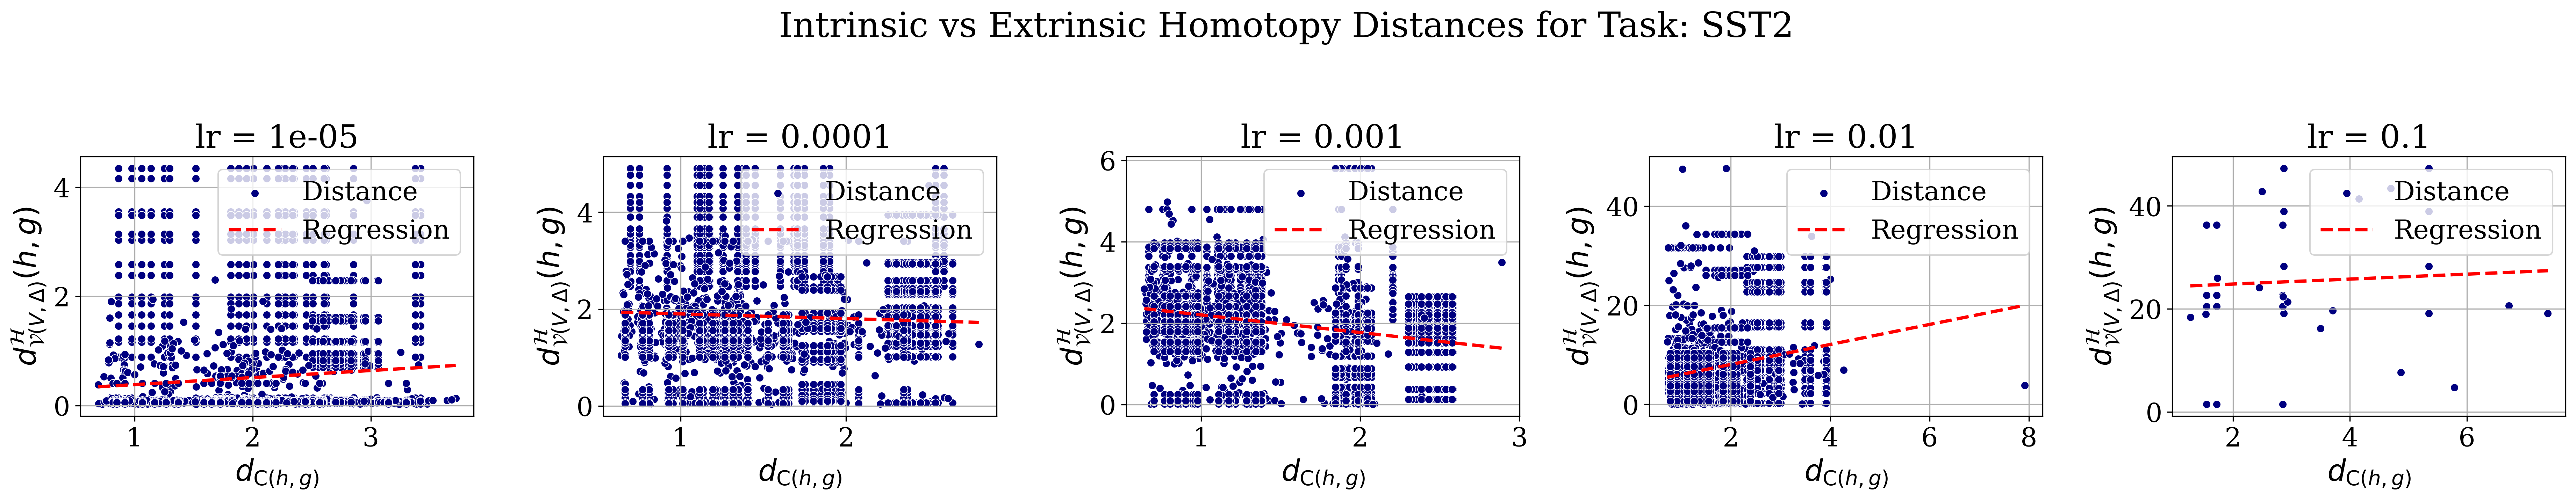
\includegraphics[width=\linewidth]{Abschlussarbeit/Pictures/intrinsic_vs_extrinsic_point_plots/PräsiDist_extr_intr_subplots_sst2.png}
	\caption{Intrinsic vs. extrinsic distances for encoder pairs on \texttt{SST-2}.}
	\label{fig:intrinsic_vs_extrinsic_sst2}
\end{figure}


For \texttt{SST-2}, we observe very low extrinsic distances for all encoder pairs at low learning rates, with no clear dependence on intrinsic distance.  
The regression lines are flat or slightly negative across learning rates \( \leq 10^{-3} \), suggesting that structurally dissimilar encoders can be aligned well in terms of task output.  
At higher learning rates (\( \geq 0.01 \)), extrinsic distances increase dramatically, while the correlation with intrinsic distance remains weak.  
This implies that for sentiment classification, intrinsic geometry does not reliably reflect task behavior, possibly due to sparse or high-level features driving classification.

\begin{figure}[H]
	\centering
	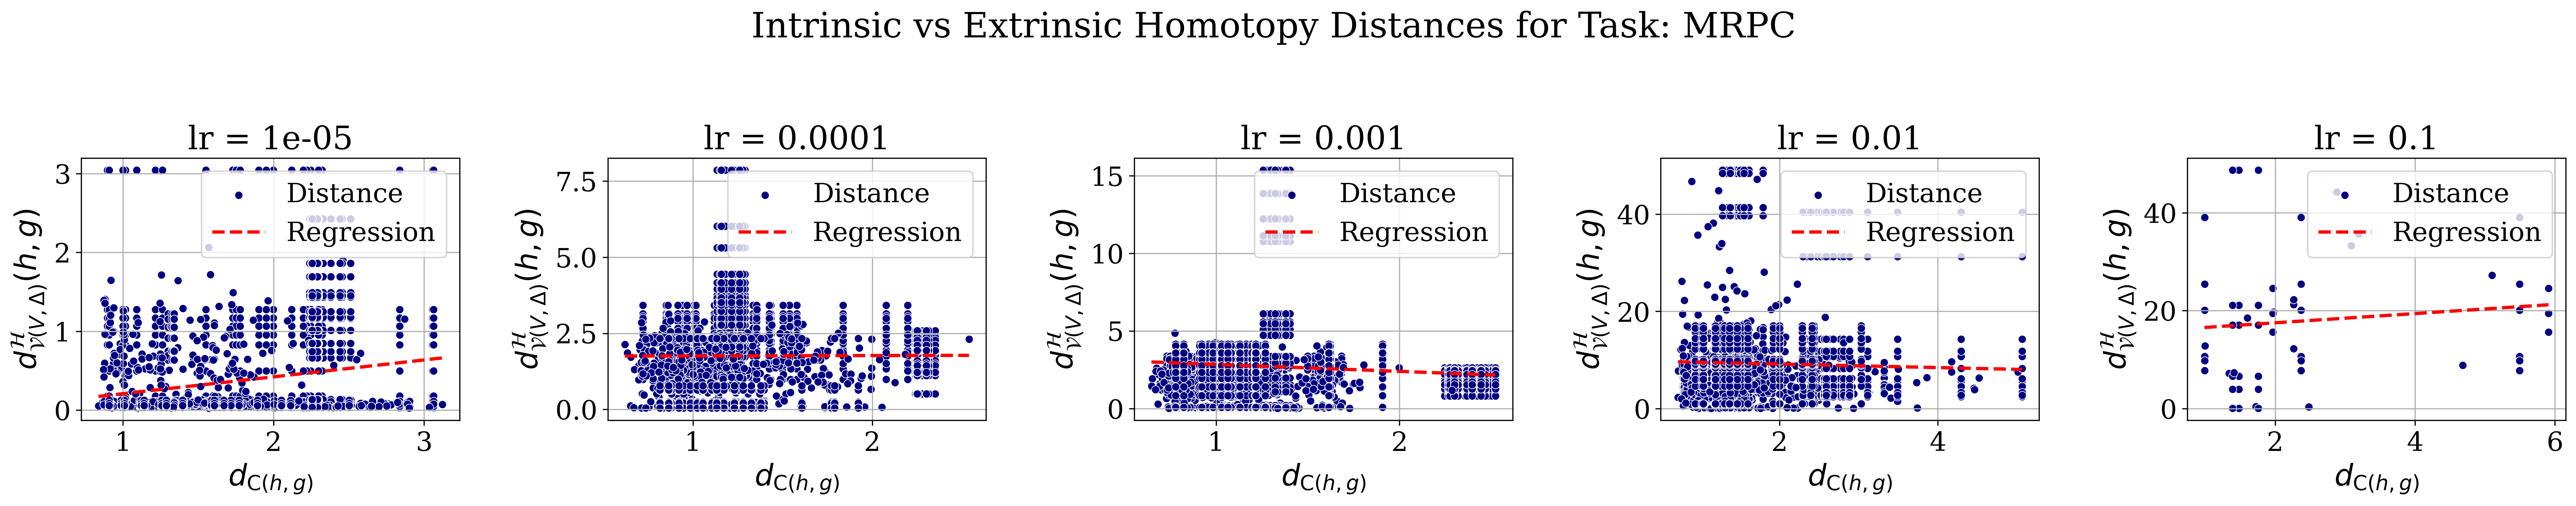
\includegraphics[width=\linewidth]{Abschlussarbeit/Pictures/intrinsic_vs_extrinsic_point_plots/PräsiDist_extr_intr_subplots_mrpc.png}
	\caption{Intrinsic vs. extrinsic distances for encoder pairs on \texttt{MRPC}.}
	\label{fig:intrinsic_vs_extrinsic_mrpc}
\end{figure}


The \texttt{MRPC} task lies between \texttt{SST-2} and \texttt{QNLI} in terms of alignment.  
At low learning rates, there is a moderate positive trend between intrinsic and extrinsic distance, with fewer extreme outliers than in \texttt{SST-2}.  
As learning rates increase, the variance in extrinsic distance grows, but the general trend persists, albeit more weakly.  
This suggests that representational similarity may be partially predictive of task behavior for paraphrase detection, but only under stable training conditions.

\begin{figure}[H]
	\centering
	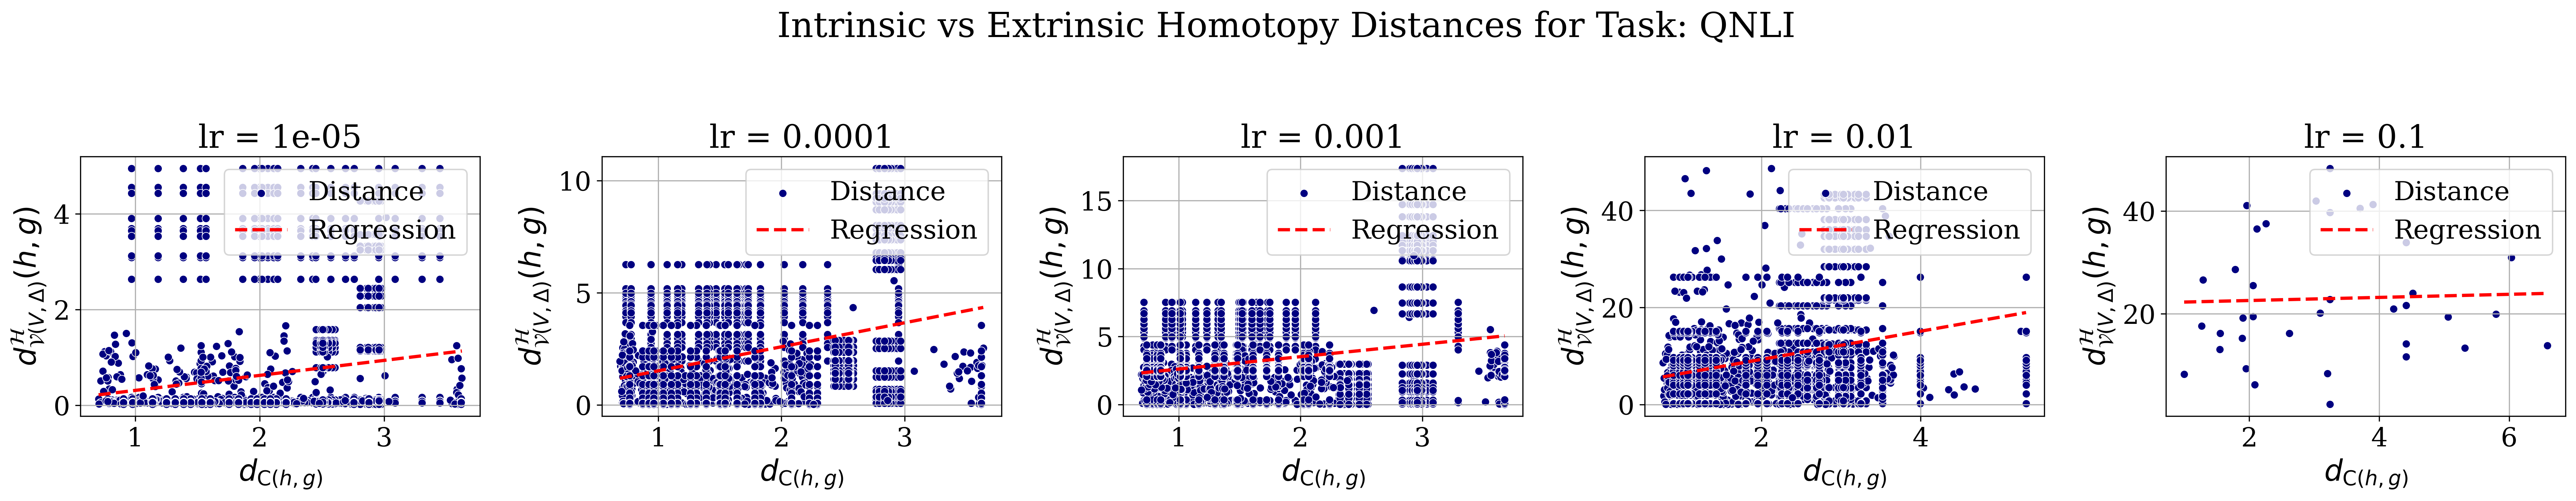
\includegraphics[width=\linewidth]{Abschlussarbeit/Pictures/intrinsic_vs_extrinsic_point_plots/PräsiDist_extr_intr_subplots_qnli.png}
	\caption{Intrinsic vs. extrinsic distances for encoder pairs on \texttt{QNLI}.}
	\label{fig:intrinsic_vs_extrinsic_qnli}
\end{figure}

\paragraph{QNLI.}
For \texttt{QNLI}, we observe a clear and consistent positive correlation between intrinsic and extrinsic distance across all learning rates.  
This indicates that encoders with similar internal representations also exhibit similar behavior on the task.  
Even at higher learning rates, where extrinsic distances increase, the regression slope remains positive and robust.  
This alignment may reflect the task's reliance on fine-grained semantic matching, which is more directly encoded in the latent space.


Overall, our findings demonstrate that the relationship between intrinsic and extrinsic homotopy is highly task-dependent.  
For some tasks, such as \texttt{QNLI}, intrinsic similarity can meaningfully predict downstream behavior.  
In others, like \texttt{SST-2}, functional similarity emerges independently of representational closeness.  
This suggests that structural alignment in representation space is neither necessary nor sufficient for downstream task alignment, and motivates task-aware evaluation of model similarity.



        \chapter{Conclusion and Future Work}\label{conc}
        In this work, we introduced a homotopy-based framework for comparing language encoder models using two types of similarity: intrinsic similarity, which focuses on internal representations, and extrinsic similarity, which considers how well models can be transformed into each other based on their task-specific outputs.
Our approach relies on learning non-linear, 1-Lipschitz-bounded transformations between model representations and estimating distances using the \(\ell^\infty\) -norm.

Compared to the affine approach by Chan et al.~\cite{chan_affine_2024}, we found that non-linear transformations lead to more homotopic model pairs, especially when trained with smaller learning rates.
This suggests that non-linear mappings allow for better alignment and reveal deeper structural relationships between encoders than affine baselines.

In the intrinsic setting, these transformations produced particularly strong results, uncovering denser connections between encoder pairs. 
In the extrinsic setting, we compared homotopy distances to performance-based similarity measures such as classification agreement and Spearman correlation. 
While high agreement often corresponded to low homotopy distance, we also observed notable exceptions: some models made similar predictions but were far apart in terms of homotopy, and others showed functional closeness despite low agreement.
This indicates that homotopy-based similarity captures deeper aspects of model behavior that are not visible from output similarity alone. 
Moreover, extrinsic homotopy distances were asymmetric transforming model \( g \) into model \( h \) was not always as easy as the reverse, highlighting a directional structure that symmetric metrics cannot capture.

We also examined how intrinsic and extrinsic homotopy relate to each other across different tasks.
While Chan et al. \cite{chan_affine_2024} suggested a close link in the affine case, our results showed that this relationship depends heavily on the task.
For example, we observed a clear positive correlation in \texttt{QNLI}, no correlation in \texttt{SST-2}, and moderate correlation in \texttt{MRPC}.
This shows that intrinsic and extrinsic similarity capture different aspects of model behavior and should be analyzed together to gain a more complete picture.

In summary, our work shows that homotopy-based similarity, especially with non-linear transformations, offers a powerful and flexible way to compare language models. 
It goes beyond simple agreement or correlation and helps reveal deeper structural relationships between models.

\paragraph{Limitations.}
Despite the promising results, this work has several limitations. 
First, our experiments were restricted to \texttt{BERT}-based models and \ac{GLUE} classification tasks, which limits the generalizability to other architectures or domains. 
Second, the method showed sensitivity to hyperparameters, particularly the learning rate, which influenced training stability and distance estimates. 
Additionally, the transformation networks were limited to simple feedforward architectures with spectral normalization, which may constrain expressiveness.

\paragraph{Future Work.}
While this study focused on language models and classification tasks from the \ac{GLUE} benchmark, our approach is broadly applicable and opens up several directions for future research.

First, one promising application lies in the field of IT security.
Since homotopy-based similarity captures structural and functional alignment between models, it could be used to detect anomalies introduced by data poisoning or backdoor attacks.
For example, poisoned models might exhibit abnormal extrinsic or intrinsic distances when compared to clean reference models, even if their test accuracy remains high.
Investigating whether homotopy measures can serve as early indicators of such manipulations could be a valuable direction for applied research.

 
While we were unable to fully reproduce Chan et al.~\cite{chan_affine_2024} reported results on held-out data, we found that our training-based measurements exhibit patterns that are broadly consistent with their findings.  
This suggests that differences in evaluation methodology, particularly the choice of data split, may partially account for the discrepancy.



%Exploring this could clarify the role of generalization in homotopy-based alignment and help distinguish between memorization and true representational similarity.

Finally, future work should address the current limitations by extending the analysis to more diverse model architectures, datasets, and transformation classes.
This includes considering multilingual models, generative tasks, and more expressive transformation networks beyond fully connected layers with spectral normalization.
        
        \cleardoublepage


	% Literaturverzeichnis in das Inhaltsverzeichnis einfügen
	\phantomsection
	\addcontentsline{toc}{chapter}{References}
      % Einfügen des Literaturverzeichnisses in das Dokument
        \bibliography{Abschlussarbeit/Text/Literatur}
         \cleardoublepage
       
       \makedeclaration
    
\end{document}
